\documentclass[G]{cpgf}

%*********** Modelo de TESE / DISSERTA\c{C}\~AO / TCC *************************
% ATEN\c{C}\~AO: N\~AO MOFICIAR A ESTRUTURA DESTE ARQUIVO.
%
% Os coment\'arios com uma s\'o porcentagem(%) s\~ao comando que podem  ser 
% incluidos descomentando-os. Para n\~ao utilizar um comando/enviroment 
% opcional basta coment\'a-los com uma porcentagem (%) simples.
%
% O Tipo de texto \'e escolhido mudando a op\c{c}\~ao de classe de documento no 
% commando \documentclass acima: 
%
%       D - Tese de doutorado
%       M - Disseta\c{c}\~ao de mestrado
%       G - Trabalho de Conclus\~ao de Curso da Gradua\c{c}\~ao
%
%
%   Atualizada em 19 de setembro de 2017
%
%*******************************************************************************
\graphicspath{{figures/}}
% Macro com novos comandos

% pacotes
\usepackage{amssymb}
\usepackage{amsmath}
\usepackage[OT2,T1]{fontenc}
\DeclareSymbolFont{cyrletters}{OT2}{wncyr}{m}{n}
\DeclareMathSymbol{\Sha}{\mathalpha}{cyrletters}{"58}
\usepackage{xspace}
\usepackage{color}
\usepackage{cancel}
\usepackage{stackengine}
\usepackage{ulem}
\usepackage{enumerate}
\usepackage{mathtools}
\usepackage{tikz}
\usepackage{tikz-3dplot}
\usepackage{pgfplots}
\usepackage{xcolor}

% Criando comandos de correcao e comentarios
\newcommand{\rem}[1]{{\color{red} \sout{#1}}} % remover texto
\newcommand{\new}[1]{{\color{blue} #1}} % Incluir texto
\newcommand{\com}[1]{{\color{ao} #1}} % Incluir coment\'ario



% bibtex path
\newcommand{\mybib}{/home/daniel/Dropbox/latex/library}

%criando novas cores
\definecolor{amethyst}{rgb}{0.6, 0.4, 0.8}
\definecolor{ao}{rgb}{0.0, 0.5, 0.0}
\definecolor{tangerine}{rgb}{1.0, 0.6, 0.4}

% encurtando comandos
\newcommand{\tx}[1]{\text{#1}}
\newcommand{\tb}[1]{\textbf{#1}}
\newcommand{\ti}[1]{\textit{#1}}
%\newcommand{\Ref}[1]{(\ref{#1})}
\newcommand{\code}[1]{\begin{semiverbatim} #1 \end{semiverbatim}}
\newcommand{\mat}[1]{\mathbf{#1}}
\newcommand{\vc}[1]{\boldsymbol{#1}}


%letras gregas
\newcommand{\Aa}{\alpha}
\newcommand{\Bb}{\beta}
\newcommand{\ow}{\omega}
\newcommand{\Ow}{\Omega}
\newcommand{\sg}{\sigma}
\newcommand{\lb}{\lambda}
\newcommand{\lbx}{\lambda_x}
\newcommand{\vep}{\varepsilon}
\newcommand{\y}{\gamma}
\newcommand{\tht}{\theta}
\newcommand{\p}{\varphi}
\newcommand{\X}{\chi}
\newcommand{\phiiw}{\hat{\phi_i}}

\newcommand{\yi}{\gamma_i}
\newcommand{\Bbi}{\beta_i}

\newcommand{\DAa}{\Delta\alpha}
\newcommand{\DBb}{\Delta\beta}
\newcommand{\Drho}{\Delta\rho}
\newcommand{\Dsg}{\Delta\sigma}
\newcommand{\DT}{\Delta \tau}

%Hamiltoniana
\newcommand{\ham}{\mathcal{H}}
\newcommand{\co}{c_0}
\newcommand{\ce}{c_{\epsilon}}
\newcommand{\cdel}{c_{\delta}}
\newcommand{\nuj}{\nu_{j}}
\newcommand{\sj}{s_{j}}
% Deltas e deltas
\newcommand{\D}{\Delta}
\newcommand{\Dt}{\Delta t}
\newcommand{\Dw}{\Delta \ow}
\newcommand{\Dx}{\Delta x}
\newcommand{\Dy}{\Delta y}
\newcommand{\Dz}{\Delta z}
\newcommand{\Dr}{\Delta r}


% Caligraficas
\newcommand{\vTau}{\mathcal{T}}
\newcommand{\cC}{\mathcal{C}}
\newcommand{\cL}{\mathcal{L}}
\newcommand{\cO}{\mathcal{O}}
\newcommand{\cR}{{\cal R}}
\newcommand{\cH}{{\cal H}}
\newcommand{\FF}{\mathcal{F}}
\newcommand{\iFF}{\mathcal{F}^{-1}}

\newcommand{\cHm}[1][m]{\cH^{(#1)} }

% conjuntos
\newcommand{\F}{\mathbb{F}}
\newcommand{\R}{\mathbb{R}}
\newcommand{\I}{\mathbb{I}}
\newcommand{\C}{\mathbb{C}}
\newcommand{\Z}{\mathbb{Z}}
\newcommand{\N}{\mathbb{N}}

\newcommand{\fM}{\mathfrak{M}}

\newcommand{\M}[1][]{\mathbb{M}#1}
\newcommand{\MR}[1][\mn]{\M[#1](\R)}

%Vetores e matrizes
\newcommand{\ve}[1][i]{\boldsymbol{\hat{e}_{#1}}}

\newcommand{\matT}[1]{\mat{#1}^T}
\newcommand{\matH}[1]{\mat{#1}^{\ast}}

\newcommand{\mA}{\mat{A}}
\newcommand{\mAi}{\mA^{-1}}
\newcommand{\mAT}{\matT{A}}
\newcommand{\mAH}{\matH{A}}

\newcommand{\cofA}[2][\mA]{\Delta^{(#1)}_{#2}}
\newcommand{\cofAij}{\cofA{ij}}

\newcommand{\mB}{\mat{B}}
\newcommand{\mBi}{\mB^{-1}}
\newcommand{\mBT}{\matT{B}}
\newcommand{\mBH}{\matH{B}}

\newcommand{\mE}{\mat{E}}
\newcommand{\mH}{\mat{H}}
\newcommand{\mHX}{\mat{H}_{\X} }
\newcommand{\mHXb}{\bar{\mat{H}}_{\X} }
\newcommand{\mR}{\mat{R}}
\newcommand{\mC}{\mat{C}}
\newcommand{\mS}{\mat{S}}
\newcommand{\mX}{\mat{X}}
\newcommand{\mY}{\mat{Y}}
\newcommand{\mO}{\mat{0}}
\newcommand{\mI}{\mat{I}}
\newcommand{\mU}{\mat{U}}
\newcommand{\mV}{\mat{V}}
\newcommand{\mW}{\mat{W}}
\newcommand{\mL}{\mat{L}}
\newcommand{\mSg}{\mat{\Sigma}}
\newcommand{\hmL}{\hat{\mL}}

\newcommand{\mHm}[1][m]{\mH^{(#1)}}

\newcommand{\aij}[1][ij]{a_{#1}}
\newcommand{\bij}[1][ij]{b_{#1}}
\newcommand{\cij}[1][ij]{c_{#1}}

\newcommand{\maij}[2][ij]{\left[\aij[#1]\right]#2}
\newcommand{\mbij}[2][ij]{\left[\bij[#1]\right]#2}

\newcommand{\mn}{_{m \times n}}
\newcommand{\nn}{_{n \times n}}
\newcommand{\n}{_{n}}
\newcommand{\mxl}{_{m \times 1}}
\newcommand{\nxl}{_{n \times 1}}

\newcommand{\vi}{\,\hat{\vc{i}}}
\newcommand{\vj}{\,\hat{\vc{j}}}
\newcommand{\vk}{\,\hat{\vc{k}}}


\newcommand{\x}{\vc{x}}
\newcommand{\vu}{\vc{u}}
\newcommand{\hvu}{\hat{\vu}}
\newcommand{\vw}{\vc{w}}
\newcommand{\vx}{\vc{x}}
\newcommand{\vv}{\vc{V}}
\newcommand{\vh}{\vc{h}}
\newcommand{\vd}{\vc{d}}
\newcommand{\hvd}{\hat{\vc{d}}}
\newcommand{\vr}{\vc{r}}
\newcommand{\vf}{\vc{f}}
\newcommand{\vt}{\vc{\t}}
\newcommand{\vht}{\hat{\vc{t}}}
\newcommand{\vp}{\vc{p}}
\newcommand{\vy}{\vc{y}}
\newcommand{\vb}{\vc{b}}
\newcommand{\vhb}{\hat{\vc{b}}}
\newcommand{\va}{\vc{a}}
\newcommand{\vn}{\vc{n}}
\newcommand{\vhn}{\hat{\vc{n}}}
\newcommand{\vO}{\vc{0}}

\newcommand{\hvn}{\hat{\vn}}
\newcommand{\hvt}{\hat{\vt}}
\newcommand{\hp}{\hat{p}}
\newcommand{\hg}{\hat{g}}
\newcommand{\fw}{\skew{4.5}\hat{f}(\omega)}
\newcommand{\pxw}{\skew{4.5}\hat{P_x}}
\newcommand{\vwf}{\skew{4.5}\hat{V}}
\newcommand{\phixw}{\hat{\phi_x}}
\newcommand{\gw}{\skew{4.5}\hat{G}}
\newcommand{\Gw}{\skew{4.5}\hat{\mathcal{G}}}
\newcommand{\pw}{\skew{4.5}\hat{P}}
\newcommand{\qw}{\skew{4.5}\hat{q}(\vc{r},\ow)}
\newcommand{\ffw}{\vc{\skew{4.5}\hat{f}}(\vc{r},\ow)}

\newcommand{\vR}{\vc{R}}
\newcommand{\vF}{\vc{F}}
\newcommand{\vZ}{\vc{Z}}
\newcommand{\vY}{\vc{Y}}
\newcommand{\vW}{\vc{W}}
\newcommand{\vA}{\vc{A}}
\newcommand{\vB}{\vc{B}}
\newcommand{\vC}{\vc{C}}
\newcommand{\vD}{\vc{D}}
\newcommand{\vM}{\vc{M}}
\newcommand{\vG}{\vc{\Gamma}}
\newcommand{\vT}{\vc{\Theta}}
\newcommand{\vP}{\vc{\Phi}}


\newcommand{\m}{\vc{m}}
\newcommand{\tm}{\tilde{\vc{m}}}
\newcommand{\mz}{\m_0}
\newcommand{\mi}[1][]{\m_{i#1}}
\newcommand{\mj}{\m_j}
\newcommand{\mii}{\mi[+1]}
\newcommand{\dm}{\delta\m}
\newcommand{\dmest}{\delta m^{\est}}


\newcommand{\h}{\vc{h}}
\newcommand{\hz}{\h_0}
\newcommand{\hii}{\h_{i+1}}
\newcommand{\hi}{\h_i}
\newcommand{\hj}{\h_j}

% Funcoes
\newcommand{\ft}[1][]{f_{#1}(t)}
\newcommand{\gt}[1][]{g_{#1}(t)}
\newcommand{\hfw}[1][]{\hf_{#1}(\ow)}
\newcommand{\hhw}[1][]{\hh_{#1}(\ow)}
\newcommand{\fx}{f(x)}
\newcommand{\fxy}{f(x,y)}
\newcommand{\Pxy}{P(x,y)}
\newcommand{\Qxy}{Q(x,y)}
\newcommand{\fxyz}{f(x,y,z)}


\newcommand{\gx}{g(x)}
\newcommand{\gxy}{g(x,y)}
\newcommand{\yt}{y(t)}
\newcommand{\xt}{x(t)}
\newcommand{\yn}{y[n]}
\newcommand{\yk}{y_k}
\newcommand{\Yn}{Y_n}
\newcommand{\wN}[1][-nk]{w_N^{#1}}
\newcommand{\xn}{x[n]}
\newcommand{\mut}[1][]{\mu_{#1}(t)}
\newcommand{\mun}[1][]{\mu_{#1}[n]}
\newcommand{\hf}{\hat f}
\newcommand{\hx}{\hat x}
\newcommand{\hh}{\hat h}
\newcommand{\sgn}{\textrm{sgn} }
\newcommand{\sinc}{\textrm{sinc} }


\newcommand{\ep}[1][\ow t]{e^{i #1}}
\newcommand{\en}[1][\ow t]{e^{-i #1}}

\newcommand{\RtR}{\R \rightarrow \R}
\newcommand{\RtC}{\R \rightarrow \C}

% trigonometria
\newcommand{\sech}{\textrm{sech}}
\newcommand{\csch}{\textrm{csch}}


% Espa\c{c}os
\newcommand{\lp}[1][p]{\ell^#1}
\newcommand{\ld}{\lp[2]}

\newcommand{\Lp}[1][p]{L^#1}
\newcommand{\Ld}{\Lp[2]}

% Operadores
\renewcommand{\d}[2][]{\,\textrm{d}^{#1}#2}
\newcommand{\dx}[1][x]{\d{#1}}
\newcommand{\diiix}{\d[3]{\x}}
\newcommand{\diix}{\d[2]{\x}}
\newcommand{\dt}{\dx[t]}
\newcommand{\dr}{\dx[r]}
\newcommand{\dvr}{\dx[\vr]}
\newcommand{\ds}{\dx[s]}
\newcommand{\dtht}{\dx[\tht]}
\newcommand{\dtau}{\dx[\tau]}
\newcommand{\dy}{\dx[y]}
\newcommand{\dz}{\dx[z]}
\newcommand{\dw}{\dx[\ow]}
\newcommand{\dA}{\dx[A]}
\newcommand{\dV}{\dx[V]}
\newcommand{\dS}{\dx[S]}
\newcommand{\dvS}{\dx[\vc{S}]}

%\newcommand{\tr}{\textrm{tr}}
\newcommand{\posto}{\textrm{posto}}
\newcommand{\rank}{\textrm{rank}}
\newcommand{\nul}{\textrm{null}}
\newcommand{\im}{\textrm{Im}}
\newcommand{\re}{\textrm{Re}}


\newcommand{\dddtt}[1][]{\frac{\partial^2 #1}{\partial t^2}}
\newcommand{\dddxx}[1][]{\frac{\partial^2 #1}{\partial x^2}}
\newcommand{\dddxi}[1][]{\frac{\partial^2 #1}{\partial x_i^2}}
\newcommand{\dddzz}[1][]{\frac{\partial^2 #1}{\partial z^2}}
\newcommand{\dddyy}[1][]{\frac{\partial^2 #1}{\partial y^2}}
\newcommand{\ddd}[2][]{\frac{\partial^2 #1}{\partial #2^2}}
\newcommand{\dddc}[3][]{\frac{\partial^2 #1}{\partial #2 \partial #3}}

\newcommand{\ddy}[1][]{\frac{\partial #1}{\partial y}}
\newcommand{\ddi}[1][]{\frac{\partial #1}{\partial i}}
\newcommand{\ddz}[1][]{\frac{\partial #1}{\partial z}}
\newcommand{\ddx}[1][]{\frac{\partial #1}{\partial x}}
\newcommand{\ddt}[1][]{\frac{\partial #1}{\partial t}}
\newcommand{\dd}[2][]{\frac{\partial #1}{\partial #2}}

\newcommand{\DD}[2][]{\frac{\dx[#1]}{\dx[#2]}}
\newcommand{\DDn}[3][n]{\frac{\d[#1]#2}{\dx[#3]^{#1}}}

\newcommand{\DDx}[1][]{\frac{\dx[#1]}{\dx}}
\newcommand{\DDt}[1][]{\frac{\dx[#1]}{\dt}}
\newcommand{\DDDtt}[1][]{\frac{\dx[]^2#1}{\dt^2}}
\newcommand{\DDw}[1][]{\frac{\dx[#1]}{\dw}}


\newcommand{\lap}[1][]{\nabla^2_{#1}}
\newcommand{\Grad}[1][]{\nabla_{#1}}
\newcommand{\Div}[1][]{\nabla_{#1} \cdot }
\newcommand{\Rot}[1][]{\nabla_{#1} \times}

\newcommand{\dk}[1][]{\delta_{#1}}
\newcommand{\del}[1][t]{\delta\!\left(#1\right)}
\newcommand{\delc}[1][n]{\delta\left[#1\right]}

\newcommand{\intifif}{\int_{-\infty}^{\infty}}
\newcommand{\intOif}{\int_{0}^{\infty}}

\newcommand{\dint}{\displaystyle\int}

\newcommand{\sumifif}[1][n]{\sum_{#1=-\infty}^{\infty}}
\newcommand{\sumOif}[1][n]{\sum_{#1=0}^{\infty}}
\newcommand{\sumuif}[1][n]{\sum_{#1=1}^{\infty}}

\newcommand{\sumON}[1][k]{\sum_{#1=0}^{N-1}}

\newcommand{\norm}[2][]{\left\Vert#2\right\Vert_{#1}}
\newcommand{\mdl}[1]{\left|#1\right|}
\newcommand{\PI}[2]{\left\langle#1,#2\right\rangle}

\newcommand{\cchts}[1]{\left[#1\right]}
\newcommand{\Cchts}[1]{\left[\begin{array}#1 \end{array}\right]}
\newcommand{\prts}[1]{\left(#1\right)}
\newcommand{\chvs}[1]{\left\{#1\right\}}
\newcommand{\Chvs}[1]{\left\{\begin{array}#1 \end{array}\right\}}
\newcommand{\Sist}[1]{\left\{\begin{array}#1 \end{array}\right.}

\newcommand{\fft}[2][]{{\cal F}^{#1}\cchts{#2}}
\newcommand{\lplc}[2][]{{\cal L}^{#1}\cchts{#2}}
\newcommand{\hilb}[2][]{{\cal H}^{#1}\cchts{#2}}

% \newcommand{\mod}{\textrm{mod}}

%ondas elasticas
\newcommand{\kz}{k_z}
\newcommand{\ky}{k_y}
\newcommand{\kx}{k_x}

\newcommand{\kAa}{k_{\Aa}}
\newcommand{\kBa}{k_{\Bb}}

\newcommand{\vua}{\vu_{\Aa}}
\newcommand{\vub}{\vu_{\Bb}}

% Diferencas finitas
\newcommand{\uijn}[3][]{u_{i#1,j#2}^{n#3}}
\newcommand{\uin}[2][]{u_{i#1}^{n#2}}


\newcommand{\kij}[2][]{K_{i#1,j#2}}
\newcommand{\Pij}[3][t]{P_{i#2,j#3}(#1)}
\newcommand{\Vxij}[3][t]{V\!x_{i#2,j#3}(#1)}
\newcommand{\Vzij}[3][t]{V\!z_{i#2,j#3}(#1)}
\newcommand{\Vxijl}[3][]{V\!x_{i#1,j#2}^{l#3}(t)}
\newcommand{\Vzijl}[3][]{V\!z_{i#1,j#2}^{l#3}(t)}
\newcommand{\qij}[3][]{q_{i#2,j#3}}
\newcommand{\fxij}[2][]{fx_{i#1,j#2}}
\newcommand{\fzij}[2][]{fz_{i#1,j#2}}
\newcommand{\Rhoij}[2][]{\rho_{i#1,j#2}}
\newcommand{\Rhoxij}[2][]{\rho x_{i#1,j#2}}
\newcommand{\Rhozij}[2][]{\rho z_{i#1,j#2}}
\newcommand{\csi}{{\xi}_i}


\newcommand{\Pijl}[3][]{P_{i#1,j#2}^{l#3}}
\newcommand{\vxijl}[3][]{vx_{i#1,j#2}^{l#3}}
\newcommand{\vzijl}[3][]{vz_{i#1,j#2}^{l#3}}
\newcommand{\fxijl}[3][]{fx_{i#1,j#2}^{l#3}}
\newcommand{\fzijl}[3][]{fz_{i#1,j#2}^{l#3}}
\newcommand{\qijl}[3][]{q_{i#1,j#2}^{l#3}}


\newcommand{\Uijn}[3][]{U_{i#1,j#2}^{n#3}}
\newcommand{\Uin}[2][]{U_{i#1}^{n#2}}
\newcommand{\Un}[1][]{U^{n#1}}
\newcommand{\Ui}[1][]{U_{i#1}}

\newcommand{\odf}[2][2N]{\partial^{[#1]}_{#2}}

\newcommand{\Kij}[1][ij]{K^{#1} }
\newcommand{\hpij}[1][ij]{\hat{p}^{#1} }
\newcommand{\hqij}[1][ij]{\hat{q}^{#1} }
\newcommand{\hvxij}[1][ij]{\hat{v}_x^{#1} }
\newcommand{\hvzij}[1][ij]{\hat{v}_z^{#1} }
\newcommand{\hfxij}[1][ij]{\hat{f}_x^{#1} }
\newcommand{\hfzij}[1][ij]{\hat{f}_z^{#1} }
\newcommand{\rhoxij}[1][ij]{\rho_{(x)}^{#1} }
\newcommand{\rhozij}[1][ij]{\rho_{(z)}^{#1} }
\newcommand{\bxij}[1][ij]{b_{(x)}^{#1} }
\newcommand{\bzij}[1][ij]{b_{(z)}^{#1} }
\newcommand{\xixi}[1][i]{\xi_x^{#1}}
\newcommand{\xizj}[1][j]{\xi_z^{#1}}


% par\'agrafos especiais
\newcounter{ex}
\newcommand{\ex}[1][\theex]{\paragraph{Exerc\'icio #1}\stepcounter{ex}}

\newcounter{eg}
\newcommand{\eg}[1][\theeg]{\paragraph{Exemplo #1}\stepcounter{eg}}

\newcounter{qu}
\newcommand{\qu}[2][\thequ]{\paragraph{Quest\~ao #1 #2}\stepcounter{qu}}

% Transformada z
\newcommand{\az}{A(Z)}
\newcommand{\bz}{B(Z)}
\newcommand{\xz}{X(Z)}
\newcommand{\yz}{Y(Z)}
\newcommand{\fz}{F(Z)}
\newcommand{\wz}{W(Z)}
\newcommand{\pz}{P(Z)}

\newcommand{\baoz}{\bar A\left(\frac{1}{Z}\right)}
\newcommand{\bboz}{\bar B\left(\frac{1}{Z}\right)}
\newcommand{\bpoz}{\bar P\left(\frac{1}{Z}\right)}

% Micelanea

\newcommand{\vMb}{\bar{\vM}}
\newcommand{\vMd}{\dot{\vM}}

\newcommand{\xb}{\bar{x}}
\newcommand{\wb}{\bar{w}}
\newcommand{\wbm}{\bar{w}_m}

\newcommand{\vph}{\vc{\hat{p}}}
\newcommand{\vxi}{\vc{\xi}}

\newcommand{\matlab}{\textsc{Matlab}\xspace}
\newcommand{\latex}{\LaTeX\xspace}

\newcommand{\Pp}[1][(\x,\ow)]{P^+#1}
\newcommand{\Pn}[1][(\x,\ow)]{P^-#1}
\newcommand{\pp}[1][(\x,t)]{p^+#1}
\newcommand{\pn}[1][(\x,t)]{p^-#1}
\newcommand{\Pxw}[1][]{P_{#1}(\x,\ow)}
\newcommand{\Pxxw}[2][]{P(\x_{#1}|\x_{#2},\ow)}
\newcommand{\Gxxw}[3][]{G^{#1}(\x_{#2}|\x_{#3},\ow)}
\newcommand{\pxt}{p(\x,t)}
\newcommand{\QED}{\begin{flushright}
                   \textit{Q.E.D. ${\scriptstyle\blacksquare}$}
                  \end{flushright}
}

\newcommand{\ubar}[1]{\underset{\bar{}}{#1}}

\newcommand{\adj}{\textrm{adj}\, }

% \newcommand{\enumroman}[2][black]{\end{frame}

% \setbeamertemplate{enumerate item}{{\color{#1}\insertenumlabel}}
% #2
% \setbeamertemplate{enumerate items}[ball]
% \renewcommand{\theenumi}{\arabic{enumi}}}







%% Inclui arquivo com pacotes extras, macros e/ou novos comandos
%% Macro com novos comandos

% pacotes
\usepackage{amssymb}
\usepackage{amsmath}
\usepackage[OT2,T1]{fontenc}
\DeclareSymbolFont{cyrletters}{OT2}{wncyr}{m}{n}
\DeclareMathSymbol{\Sha}{\mathalpha}{cyrletters}{"58}
\usepackage{xspace}
\usepackage{color}
\usepackage{cancel}
\usepackage{stackengine}
\usepackage{ulem}
\usepackage{enumerate}
\usepackage{mathtools}
\usepackage{tikz}
\usepackage{tikz-3dplot}
\usepackage{pgfplots}
\usepackage{xcolor}

% Criando comandos de correcao e comentarios
\newcommand{\rem}[1]{{\color{red} \sout{#1}}} % remover texto
\newcommand{\new}[1]{{\color{blue} #1}} % Incluir texto
\newcommand{\com}[1]{{\color{ao} #1}} % Incluir coment\'ario



% bibtex path
\newcommand{\mybib}{/home/daniel/Dropbox/latex/library}

%criando novas cores
\definecolor{amethyst}{rgb}{0.6, 0.4, 0.8}
\definecolor{ao}{rgb}{0.0, 0.5, 0.0}
\definecolor{tangerine}{rgb}{1.0, 0.6, 0.4}

% encurtando comandos
\newcommand{\tx}[1]{\text{#1}}
\newcommand{\tb}[1]{\textbf{#1}}
\newcommand{\ti}[1]{\textit{#1}}
%\newcommand{\Ref}[1]{(\ref{#1})}
\newcommand{\code}[1]{\begin{semiverbatim} #1 \end{semiverbatim}}
\newcommand{\mat}[1]{\mathbf{#1}}
\newcommand{\vc}[1]{\boldsymbol{#1}}


%letras gregas
\newcommand{\Aa}{\alpha}
\newcommand{\Bb}{\beta}
\newcommand{\ow}{\omega}
\newcommand{\Ow}{\Omega}
\newcommand{\sg}{\sigma}
\newcommand{\lb}{\lambda}
\newcommand{\lbx}{\lambda_x}
\newcommand{\vep}{\varepsilon}
\newcommand{\y}{\gamma}
\newcommand{\tht}{\theta}
\newcommand{\p}{\varphi}
\newcommand{\X}{\chi}
\newcommand{\phiiw}{\hat{\phi_i}}

\newcommand{\yi}{\gamma_i}
\newcommand{\Bbi}{\beta_i}

\newcommand{\DAa}{\Delta\alpha}
\newcommand{\DBb}{\Delta\beta}
\newcommand{\Drho}{\Delta\rho}
\newcommand{\Dsg}{\Delta\sigma}
\newcommand{\DT}{\Delta \tau}

%Hamiltoniana
\newcommand{\ham}{\mathcal{H}}
\newcommand{\co}{c_0}
\newcommand{\ce}{c_{\epsilon}}
\newcommand{\cdel}{c_{\delta}}
\newcommand{\nuj}{\nu_{j}}
\newcommand{\sj}{s_{j}}
% Deltas e deltas
\newcommand{\D}{\Delta}
\newcommand{\Dt}{\Delta t}
\newcommand{\Dw}{\Delta \ow}
\newcommand{\Dx}{\Delta x}
\newcommand{\Dy}{\Delta y}
\newcommand{\Dz}{\Delta z}
\newcommand{\Dr}{\Delta r}


% Caligraficas
\newcommand{\vTau}{\mathcal{T}}
\newcommand{\cC}{\mathcal{C}}
\newcommand{\cL}{\mathcal{L}}
\newcommand{\cO}{\mathcal{O}}
\newcommand{\cR}{{\cal R}}
\newcommand{\cH}{{\cal H}}
\newcommand{\FF}{\mathcal{F}}
\newcommand{\iFF}{\mathcal{F}^{-1}}

\newcommand{\cHm}[1][m]{\cH^{(#1)} }

% conjuntos
\newcommand{\F}{\mathbb{F}}
\newcommand{\R}{\mathbb{R}}
\newcommand{\I}{\mathbb{I}}
\newcommand{\C}{\mathbb{C}}
\newcommand{\Z}{\mathbb{Z}}
\newcommand{\N}{\mathbb{N}}

\newcommand{\fM}{\mathfrak{M}}

\newcommand{\M}[1][]{\mathbb{M}#1}
\newcommand{\MR}[1][\mn]{\M[#1](\R)}

%Vetores e matrizes
\newcommand{\ve}[1][i]{\boldsymbol{\hat{e}_{#1}}}

\newcommand{\matT}[1]{\mat{#1}^T}
\newcommand{\matH}[1]{\mat{#1}^{\ast}}

\newcommand{\mA}{\mat{A}}
\newcommand{\mAi}{\mA^{-1}}
\newcommand{\mAT}{\matT{A}}
\newcommand{\mAH}{\matH{A}}

\newcommand{\cofA}[2][\mA]{\Delta^{(#1)}_{#2}}
\newcommand{\cofAij}{\cofA{ij}}

\newcommand{\mB}{\mat{B}}
\newcommand{\mBi}{\mB^{-1}}
\newcommand{\mBT}{\matT{B}}
\newcommand{\mBH}{\matH{B}}

\newcommand{\mE}{\mat{E}}
\newcommand{\mH}{\mat{H}}
\newcommand{\mHX}{\mat{H}_{\X} }
\newcommand{\mHXb}{\bar{\mat{H}}_{\X} }
\newcommand{\mR}{\mat{R}}
\newcommand{\mC}{\mat{C}}
\newcommand{\mS}{\mat{S}}
\newcommand{\mX}{\mat{X}}
\newcommand{\mY}{\mat{Y}}
\newcommand{\mO}{\mat{0}}
\newcommand{\mI}{\mat{I}}
\newcommand{\mU}{\mat{U}}
\newcommand{\mV}{\mat{V}}
\newcommand{\mW}{\mat{W}}
\newcommand{\mL}{\mat{L}}
\newcommand{\mSg}{\mat{\Sigma}}
\newcommand{\hmL}{\hat{\mL}}

\newcommand{\mHm}[1][m]{\mH^{(#1)}}

\newcommand{\aij}[1][ij]{a_{#1}}
\newcommand{\bij}[1][ij]{b_{#1}}
\newcommand{\cij}[1][ij]{c_{#1}}

\newcommand{\maij}[2][ij]{\left[\aij[#1]\right]#2}
\newcommand{\mbij}[2][ij]{\left[\bij[#1]\right]#2}

\newcommand{\mn}{_{m \times n}}
\newcommand{\nn}{_{n \times n}}
\newcommand{\n}{_{n}}
\newcommand{\mxl}{_{m \times 1}}
\newcommand{\nxl}{_{n \times 1}}

\newcommand{\vi}{\,\hat{\vc{i}}}
\newcommand{\vj}{\,\hat{\vc{j}}}
\newcommand{\vk}{\,\hat{\vc{k}}}


\newcommand{\x}{\vc{x}}
\newcommand{\vu}{\vc{u}}
\newcommand{\hvu}{\hat{\vu}}
\newcommand{\vw}{\vc{w}}
\newcommand{\vx}{\vc{x}}
\newcommand{\vv}{\vc{V}}
\newcommand{\vh}{\vc{h}}
\newcommand{\vd}{\vc{d}}
\newcommand{\hvd}{\hat{\vc{d}}}
\newcommand{\vr}{\vc{r}}
\newcommand{\vf}{\vc{f}}
\newcommand{\vt}{\vc{\t}}
\newcommand{\vht}{\hat{\vc{t}}}
\newcommand{\vp}{\vc{p}}
\newcommand{\vy}{\vc{y}}
\newcommand{\vb}{\vc{b}}
\newcommand{\vhb}{\hat{\vc{b}}}
\newcommand{\va}{\vc{a}}
\newcommand{\vn}{\vc{n}}
\newcommand{\vhn}{\hat{\vc{n}}}
\newcommand{\vO}{\vc{0}}

\newcommand{\hvn}{\hat{\vn}}
\newcommand{\hvt}{\hat{\vt}}
\newcommand{\hp}{\hat{p}}
\newcommand{\hg}{\hat{g}}
\newcommand{\fw}{\skew{4.5}\hat{f}(\omega)}
\newcommand{\pxw}{\skew{4.5}\hat{P_x}}
\newcommand{\vwf}{\skew{4.5}\hat{V}}
\newcommand{\phixw}{\hat{\phi_x}}
\newcommand{\gw}{\skew{4.5}\hat{G}}
\newcommand{\Gw}{\skew{4.5}\hat{\mathcal{G}}}
\newcommand{\pw}{\skew{4.5}\hat{P}}
\newcommand{\qw}{\skew{4.5}\hat{q}(\vc{r},\ow)}
\newcommand{\ffw}{\vc{\skew{4.5}\hat{f}}(\vc{r},\ow)}

\newcommand{\vR}{\vc{R}}
\newcommand{\vF}{\vc{F}}
\newcommand{\vZ}{\vc{Z}}
\newcommand{\vY}{\vc{Y}}
\newcommand{\vW}{\vc{W}}
\newcommand{\vA}{\vc{A}}
\newcommand{\vB}{\vc{B}}
\newcommand{\vC}{\vc{C}}
\newcommand{\vD}{\vc{D}}
\newcommand{\vM}{\vc{M}}
\newcommand{\vG}{\vc{\Gamma}}
\newcommand{\vT}{\vc{\Theta}}
\newcommand{\vP}{\vc{\Phi}}


\newcommand{\m}{\vc{m}}
\newcommand{\tm}{\tilde{\vc{m}}}
\newcommand{\mz}{\m_0}
\newcommand{\mi}[1][]{\m_{i#1}}
\newcommand{\mj}{\m_j}
\newcommand{\mii}{\mi[+1]}
\newcommand{\dm}{\delta\m}
\newcommand{\dmest}{\delta m^{\est}}


\newcommand{\h}{\vc{h}}
\newcommand{\hz}{\h_0}
\newcommand{\hii}{\h_{i+1}}
\newcommand{\hi}{\h_i}
\newcommand{\hj}{\h_j}

% Funcoes
\newcommand{\ft}[1][]{f_{#1}(t)}
\newcommand{\gt}[1][]{g_{#1}(t)}
\newcommand{\hfw}[1][]{\hf_{#1}(\ow)}
\newcommand{\hhw}[1][]{\hh_{#1}(\ow)}
\newcommand{\fx}{f(x)}
\newcommand{\fxy}{f(x,y)}
\newcommand{\Pxy}{P(x,y)}
\newcommand{\Qxy}{Q(x,y)}
\newcommand{\fxyz}{f(x,y,z)}


\newcommand{\gx}{g(x)}
\newcommand{\gxy}{g(x,y)}
\newcommand{\yt}{y(t)}
\newcommand{\xt}{x(t)}
\newcommand{\yn}{y[n]}
\newcommand{\yk}{y_k}
\newcommand{\Yn}{Y_n}
\newcommand{\wN}[1][-nk]{w_N^{#1}}
\newcommand{\xn}{x[n]}
\newcommand{\mut}[1][]{\mu_{#1}(t)}
\newcommand{\mun}[1][]{\mu_{#1}[n]}
\newcommand{\hf}{\hat f}
\newcommand{\hx}{\hat x}
\newcommand{\hh}{\hat h}
\newcommand{\sgn}{\textrm{sgn} }
\newcommand{\sinc}{\textrm{sinc} }


\newcommand{\ep}[1][\ow t]{e^{i #1}}
\newcommand{\en}[1][\ow t]{e^{-i #1}}

\newcommand{\RtR}{\R \rightarrow \R}
\newcommand{\RtC}{\R \rightarrow \C}

% trigonometria
\newcommand{\sech}{\textrm{sech}}
\newcommand{\csch}{\textrm{csch}}


% Espa\c{c}os
\newcommand{\lp}[1][p]{\ell^#1}
\newcommand{\ld}{\lp[2]}

\newcommand{\Lp}[1][p]{L^#1}
\newcommand{\Ld}{\Lp[2]}

% Operadores
\renewcommand{\d}[2][]{\,\textrm{d}^{#1}#2}
\newcommand{\dx}[1][x]{\d{#1}}
\newcommand{\diiix}{\d[3]{\x}}
\newcommand{\diix}{\d[2]{\x}}
\newcommand{\dt}{\dx[t]}
\newcommand{\dr}{\dx[r]}
\newcommand{\dvr}{\dx[\vr]}
\newcommand{\ds}{\dx[s]}
\newcommand{\dtht}{\dx[\tht]}
\newcommand{\dtau}{\dx[\tau]}
\newcommand{\dy}{\dx[y]}
\newcommand{\dz}{\dx[z]}
\newcommand{\dw}{\dx[\ow]}
\newcommand{\dA}{\dx[A]}
\newcommand{\dV}{\dx[V]}
\newcommand{\dS}{\dx[S]}
\newcommand{\dvS}{\dx[\vc{S}]}

%\newcommand{\tr}{\textrm{tr}}
\newcommand{\posto}{\textrm{posto}}
\newcommand{\rank}{\textrm{rank}}
\newcommand{\nul}{\textrm{null}}
\newcommand{\im}{\textrm{Im}}
\newcommand{\re}{\textrm{Re}}


\newcommand{\dddtt}[1][]{\frac{\partial^2 #1}{\partial t^2}}
\newcommand{\dddxx}[1][]{\frac{\partial^2 #1}{\partial x^2}}
\newcommand{\dddxi}[1][]{\frac{\partial^2 #1}{\partial x_i^2}}
\newcommand{\dddzz}[1][]{\frac{\partial^2 #1}{\partial z^2}}
\newcommand{\dddyy}[1][]{\frac{\partial^2 #1}{\partial y^2}}
\newcommand{\ddd}[2][]{\frac{\partial^2 #1}{\partial #2^2}}
\newcommand{\dddc}[3][]{\frac{\partial^2 #1}{\partial #2 \partial #3}}

\newcommand{\ddy}[1][]{\frac{\partial #1}{\partial y}}
\newcommand{\ddi}[1][]{\frac{\partial #1}{\partial i}}
\newcommand{\ddz}[1][]{\frac{\partial #1}{\partial z}}
\newcommand{\ddx}[1][]{\frac{\partial #1}{\partial x}}
\newcommand{\ddt}[1][]{\frac{\partial #1}{\partial t}}
\newcommand{\dd}[2][]{\frac{\partial #1}{\partial #2}}

\newcommand{\DD}[2][]{\frac{\dx[#1]}{\dx[#2]}}
\newcommand{\DDn}[3][n]{\frac{\d[#1]#2}{\dx[#3]^{#1}}}

\newcommand{\DDx}[1][]{\frac{\dx[#1]}{\dx}}
\newcommand{\DDt}[1][]{\frac{\dx[#1]}{\dt}}
\newcommand{\DDDtt}[1][]{\frac{\dx[]^2#1}{\dt^2}}
\newcommand{\DDw}[1][]{\frac{\dx[#1]}{\dw}}


\newcommand{\lap}[1][]{\nabla^2_{#1}}
\newcommand{\Grad}[1][]{\nabla_{#1}}
\newcommand{\Div}[1][]{\nabla_{#1} \cdot }
\newcommand{\Rot}[1][]{\nabla_{#1} \times}

\newcommand{\dk}[1][]{\delta_{#1}}
\newcommand{\del}[1][t]{\delta\!\left(#1\right)}
\newcommand{\delc}[1][n]{\delta\left[#1\right]}

\newcommand{\intifif}{\int_{-\infty}^{\infty}}
\newcommand{\intOif}{\int_{0}^{\infty}}

\newcommand{\dint}{\displaystyle\int}

\newcommand{\sumifif}[1][n]{\sum_{#1=-\infty}^{\infty}}
\newcommand{\sumOif}[1][n]{\sum_{#1=0}^{\infty}}
\newcommand{\sumuif}[1][n]{\sum_{#1=1}^{\infty}}

\newcommand{\sumON}[1][k]{\sum_{#1=0}^{N-1}}

\newcommand{\norm}[2][]{\left\Vert#2\right\Vert_{#1}}
\newcommand{\mdl}[1]{\left|#1\right|}
\newcommand{\PI}[2]{\left\langle#1,#2\right\rangle}

\newcommand{\cchts}[1]{\left[#1\right]}
\newcommand{\Cchts}[1]{\left[\begin{array}#1 \end{array}\right]}
\newcommand{\prts}[1]{\left(#1\right)}
\newcommand{\chvs}[1]{\left\{#1\right\}}
\newcommand{\Chvs}[1]{\left\{\begin{array}#1 \end{array}\right\}}
\newcommand{\Sist}[1]{\left\{\begin{array}#1 \end{array}\right.}

\newcommand{\fft}[2][]{{\cal F}^{#1}\cchts{#2}}
\newcommand{\lplc}[2][]{{\cal L}^{#1}\cchts{#2}}
\newcommand{\hilb}[2][]{{\cal H}^{#1}\cchts{#2}}

% \newcommand{\mod}{\textrm{mod}}

%ondas elasticas
\newcommand{\kz}{k_z}
\newcommand{\ky}{k_y}
\newcommand{\kx}{k_x}

\newcommand{\kAa}{k_{\Aa}}
\newcommand{\kBa}{k_{\Bb}}

\newcommand{\vua}{\vu_{\Aa}}
\newcommand{\vub}{\vu_{\Bb}}

% Diferencas finitas
\newcommand{\uijn}[3][]{u_{i#1,j#2}^{n#3}}
\newcommand{\uin}[2][]{u_{i#1}^{n#2}}


\newcommand{\kij}[2][]{K_{i#1,j#2}}
\newcommand{\Pij}[3][t]{P_{i#2,j#3}(#1)}
\newcommand{\Vxij}[3][t]{V\!x_{i#2,j#3}(#1)}
\newcommand{\Vzij}[3][t]{V\!z_{i#2,j#3}(#1)}
\newcommand{\Vxijl}[3][]{V\!x_{i#1,j#2}^{l#3}(t)}
\newcommand{\Vzijl}[3][]{V\!z_{i#1,j#2}^{l#3}(t)}
\newcommand{\qij}[3][]{q_{i#2,j#3}}
\newcommand{\fxij}[2][]{fx_{i#1,j#2}}
\newcommand{\fzij}[2][]{fz_{i#1,j#2}}
\newcommand{\Rhoij}[2][]{\rho_{i#1,j#2}}
\newcommand{\Rhoxij}[2][]{\rho x_{i#1,j#2}}
\newcommand{\Rhozij}[2][]{\rho z_{i#1,j#2}}
\newcommand{\csi}{{\xi}_i}


\newcommand{\Pijl}[3][]{P_{i#1,j#2}^{l#3}}
\newcommand{\vxijl}[3][]{vx_{i#1,j#2}^{l#3}}
\newcommand{\vzijl}[3][]{vz_{i#1,j#2}^{l#3}}
\newcommand{\fxijl}[3][]{fx_{i#1,j#2}^{l#3}}
\newcommand{\fzijl}[3][]{fz_{i#1,j#2}^{l#3}}
\newcommand{\qijl}[3][]{q_{i#1,j#2}^{l#3}}


\newcommand{\Uijn}[3][]{U_{i#1,j#2}^{n#3}}
\newcommand{\Uin}[2][]{U_{i#1}^{n#2}}
\newcommand{\Un}[1][]{U^{n#1}}
\newcommand{\Ui}[1][]{U_{i#1}}

\newcommand{\odf}[2][2N]{\partial^{[#1]}_{#2}}

\newcommand{\Kij}[1][ij]{K^{#1} }
\newcommand{\hpij}[1][ij]{\hat{p}^{#1} }
\newcommand{\hqij}[1][ij]{\hat{q}^{#1} }
\newcommand{\hvxij}[1][ij]{\hat{v}_x^{#1} }
\newcommand{\hvzij}[1][ij]{\hat{v}_z^{#1} }
\newcommand{\hfxij}[1][ij]{\hat{f}_x^{#1} }
\newcommand{\hfzij}[1][ij]{\hat{f}_z^{#1} }
\newcommand{\rhoxij}[1][ij]{\rho_{(x)}^{#1} }
\newcommand{\rhozij}[1][ij]{\rho_{(z)}^{#1} }
\newcommand{\bxij}[1][ij]{b_{(x)}^{#1} }
\newcommand{\bzij}[1][ij]{b_{(z)}^{#1} }
\newcommand{\xixi}[1][i]{\xi_x^{#1}}
\newcommand{\xizj}[1][j]{\xi_z^{#1}}


% par\'agrafos especiais
\newcounter{ex}
\newcommand{\ex}[1][\theex]{\paragraph{Exerc\'icio #1}\stepcounter{ex}}

\newcounter{eg}
\newcommand{\eg}[1][\theeg]{\paragraph{Exemplo #1}\stepcounter{eg}}

\newcounter{qu}
\newcommand{\qu}[2][\thequ]{\paragraph{Quest\~ao #1 #2}\stepcounter{qu}}

% Transformada z
\newcommand{\az}{A(Z)}
\newcommand{\bz}{B(Z)}
\newcommand{\xz}{X(Z)}
\newcommand{\yz}{Y(Z)}
\newcommand{\fz}{F(Z)}
\newcommand{\wz}{W(Z)}
\newcommand{\pz}{P(Z)}

\newcommand{\baoz}{\bar A\left(\frac{1}{Z}\right)}
\newcommand{\bboz}{\bar B\left(\frac{1}{Z}\right)}
\newcommand{\bpoz}{\bar P\left(\frac{1}{Z}\right)}

% Micelanea

\newcommand{\vMb}{\bar{\vM}}
\newcommand{\vMd}{\dot{\vM}}

\newcommand{\xb}{\bar{x}}
\newcommand{\wb}{\bar{w}}
\newcommand{\wbm}{\bar{w}_m}

\newcommand{\vph}{\vc{\hat{p}}}
\newcommand{\vxi}{\vc{\xi}}

\newcommand{\matlab}{\textsc{Matlab}\xspace}
\newcommand{\latex}{\LaTeX\xspace}

\newcommand{\Pp}[1][(\x,\ow)]{P^+#1}
\newcommand{\Pn}[1][(\x,\ow)]{P^-#1}
\newcommand{\pp}[1][(\x,t)]{p^+#1}
\newcommand{\pn}[1][(\x,t)]{p^-#1}
\newcommand{\Pxw}[1][]{P_{#1}(\x,\ow)}
\newcommand{\Pxxw}[2][]{P(\x_{#1}|\x_{#2},\ow)}
\newcommand{\Gxxw}[3][]{G^{#1}(\x_{#2}|\x_{#3},\ow)}
\newcommand{\pxt}{p(\x,t)}
\newcommand{\QED}{\begin{flushright}
                   \textit{Q.E.D. ${\scriptstyle\blacksquare}$}
                  \end{flushright}
}

\newcommand{\ubar}[1]{\underset{\bar{}}{#1}}

\newcommand{\adj}{\textrm{adj}\, }

% \newcommand{\enumroman}[2][black]{\end{frame}

% \setbeamertemplate{enumerate item}{{\color{#1}\insertenumlabel}}
% #2
% \setbeamertemplate{enumerate items}[ball]
% \renewcommand{\theenumi}{\arabic{enumi}}}








\begin{document}

%%%%%%%%%% - INFORMAÇÕES - %%%%%%%%%%%%%%%%%%%%
\title{Multi Convolução: Função Retangular}
\author{LUCAS DE CASTRO COSTA} % COLOQUE O SEU NOME EM CAIXA ALTA !!!!
\date{2021}

%% Comandos abaixo recebem 3 entadas: nome (incluindo t\'itulo), 
%% afilia\c{c}\~ao e genero (H - homem; M- mulher)
%\advisor{Prof. Dr. Lourenildo Williame Barbosa Leite}{Universidade Federal do Pará}{H}
%\coadvisor{}{}{H}


%% Comandos abaixo recebem 2 entradas: nome (incluindo t\'itulo), 
%% afilia\c{c}\~ao.
%% Se o menbro 2 da banca for coorientador usar op\c{c}\~ao [co] 
%\bancadois[co]{Prof. Dr. Alberto Santos Dummont}{Universidade Federal de Lugar 
%Nenhum}
% \bancadois{Prof. Dr. Daniel Leal Macedo}{Universidade Federal do Pará}
% \bancatres{Dr. Wildney Wallacy da Silva Vieira}{Universidade Federal do Pará}
% \bancaquatro{Profa. Dra. Ellen de Nazar\'e Souza Gomes Costa Corr\^ea Machado Alves Martins da Silva}{Universidade Federal do Rio Grande do Norte}
% \bancacinco{Prof. Dr. S\'o Isso}{Universidade Federal do Pará}


%% Colocar palavras chaves do trabalho
% \chaves{Sísmica. Processamento. Imageamento. Difração. Exploração.}
% \keys{Seismic. Processing. Imaging. difraction. Exploration.}

%%%%%%%%%% - PARTES PRETEXTUAIS - %%%%%%%%%%%%%%%%%%%%

\capa %% Obrigatorio
%\rosto  %% Obrigatorio

%% Ficha catalogr\'afica. Comentar comando abaixo quando for imprimir, pois, a 
%% ficha catalogr\'afica deve ser impressa no verso da folha de rosto. 
%% Descomentar ao fazer a vers\~ao eletr\^onica do TCC. A ficha catalogr\'afica
%% deve ser obtida previamente no formato pdf
% \includepdf[pages=-,pagecommand={},width=\textwidth]{FICAT_MURILO.pdf} % FICHA CATALOGRAFICA
% \includepdf[keepaspectratio]{aprovacao.pdf}

% \aprovacao{17 de Dezembro de 2018} %%Obrigatorio

%% Opcional
% \dedicatoria{A gravidade explica os movimentos dos planetas, mas não pode explicar quem colocou os planetas em movimento. Deus governa todas as coisas e sabe tudo que é ou que pode ser feito. Isaac Newton}

%% Agradecimentos (opcional), epigrafe (opcional), resumo (Obrigatorio), 
%% abstract (Obrigatorio)
%%%%%%%%%%%%%%%%%%%%%%%%%%%%%%%%%%%%%%%%%
% \begin{agradecimentos}
% 
% \vspace{+3.0cm}

% Ao orientador, Prof. Dr. Lourenildo W. B. Leite, por todo o conhecimento e experi\^{e}ncia repassada ao longo destes anos de conviv\^{e}ncia, e por todo o apoio para que este trabalho se tornasse realizável.
% 
% Ao Dr. Wildney W. S. Vieira por sua colabora\c{c}\~{a}o neste trabalho com uma ajuda preciosa na programação computacional e no processamento de dados sísmicos.
% 
% % Ao Prof. Dr. Daniel Leal Macedo e ao Prof. Dr. José Jadsom Sampaio de Figueiredo por participarem da Banca Examinadora, e pelas sugestões para a melhora deste relatório e sua apresentação.
% 
% Ao corpo docente da Graduação em Geofísica da UFPA por todo o conhecimento repassado para o meu desenvolvimento intelectual, científico e técnico.
% 
% Aos meus pais Modesto Diociesse e Joana Cunha pelo apoio familiar nestes anos de estudo.
% 
% Aos familiares que contribuíram de maneira direta para a execução deste trabalho, em especial meu tio Doval Cunha por todo apoio durante minha graduação, a meus avós Manoel Souza e Teresinha Cunha pelo carinho e cuidado.
% 
% Aos amigos Larissa Almeida, Alexandre Cavalcante, Arthur Rodrigues, Sheyla Machado, Melina Silva pelo apoio neste trabalho.
% 
% Aos amigos de graduação e da pós graduação em geofísica, e em especial Gabriel Bricio, Antônio Leite, Rayle Cristine, Karolina Correia, Cesar Pessoa, Fernando Andrade e Igor de Jesus.
% 
% Agradeço ao Bom Deus.

% \end{agradecimentos}

%%%%%%%% EPIGRAFE - OPCIONAL %%%%%%%%%%%%%%%%%%%%%%%%%%%%%%%%
%\newpage
%\thispagestyle{empty}
%\vspace*{\fill}
%\begin{citacao}
%	Jesus é a salvação! Jesus é a salvação! Jesus é a salvação! Jesus é a salvação! Jesus é a salvação! Jesus é a salvação! Jesus é a salvação! Jesus é a salvação! Jesus é a salvação! Jesus é a salvação! Jesus é a salvação! Jesus é a salvação! Jesus é a salvação! Jesus é a salvação! Jesus é a salvação! Jesus é a salvação! Jesus é a salvação! Jesus é a salvação! Jesus é a salvação! Jesus é a salvação! Jesus é a salvação! Jesus é a salvação! Jesus é a salvação! Jesus é a salvação! Jesus é a salvação! Jesus é a salvação! Jesus é a salvação! Jesus é a salvação! Jesus é a salvação! Jesus é a salvação! Jesus é a salvação! Jesus é a salvação! Jesus é a salvação! Jesus é a salvação! Jesus é a salvação! Jesus é a salvação! 
%	
%	{\hfill Albert Einstein.}
%\end{citacao}
%
%\newpage
%
%%%%%%%%% RESUMO - OBRIGATORIO %%%%%%%%%%%%%%%%%%%%%%%%%%%%%%%
% \begin{resumo}
% O conteúdo de uma seção sísmica pode ser resumido em ruídos diversos, reflexões, difrações e artefatos. 
% Para esta análise tomamos por base seções sísmicas marinhas da bacia do Jequitinhonha, localizada ao leste do estado da Bahia. 
% O objetivo geral deste trabalho foi o estudo e a aplicação de princípios básicos e fundamentais que descrevem o fenômeno de difração do ponto de vista sísmico para a modelagem e imageamento da subsuperfície, e tomamos como literatura inicial o trabalho clássico do autor Trorey.
% Como objetivo específico foi desenvolver programas em Matlab para a modelagem por difração para se obter as respostas sísmicas de refletores finitos simulando situações típicas encontradas na geologia, como estratos, grabens, horsts, falhas. 
% Neste trabalho nos limitamos a analisar segmentos horizontais curtos e pontuais, e levando em consideração apenas seções afastamento-nulo. 
% Foram desenvolvidos nove modelos geológicos para aplicar a teoria de Trorey, e dentre eles, dois modelos baseados na linha sísmica $214-266$ da bacia do Jequitinhonha. 
% A teoria de Trorey para o fenômeno difração-reflexão é consistente, elegante e simples para explicar feições e artefatos das seções sísmicas, e se baseia no teorema de Green no espaço que explica devidamente o fenômeno físico.
% Para sistematizar o estudo, foram também aplicadas as migrações no tempo dos tipos Kirchhoff e por deslocamento-de-fase (ambas usando o SU), com a finalidade de obter imagens consistentes com a teoria que descreve o colapso de difrações.
% Como conclusão, se observou na implementação que o método é simples para aplicação, e que se pode modelar rapidamente uma seção sísmica com muitos detalhes estruturais, como falhas, sinclinais, anticlinais, horsts, grabens, desde que se discretize bem a estrutura no domínio geológico (espaço). 
% Outra observação muito importante nas conclusões foi sobre a geração de artefatos nas seções modeladas pelo encurvamento da frente de onda ao redor da borda da estrutura, o que caracteriza as difrações. 
% Como trabalho futuro podemos considerar o desenvolvimento da modelagem e inversão de seções sísmicas complexas baseadas em interpretações geológicas importantes na exploração de petróleo, com a finalidade de melhor explicar esta interpretação de forma fisicamente (sismicamente) plausível e consistente, que é um dos objetivos da geofísica.
% \end{resumo}

%%%%%%%%% ABSTRACT - OBRIGATORIO %%%%%%%%%%%%%%%%%%%%%%%%%%%%%%%
% \begin{abstract}
% The contents of a seismic section can be summarized in various noises, reflections, diffractions and artifacts.
% For this analysis we took as a base marine seismic sections of the basin called Jequitinhonha, located to the east of the state of Bahia. The general objective was the study and application of basic and fundamental principles that describe the phenomenon of diffraction from the seismic point of view for the modeling and imaging of the subsurface according to the classic author Trorey.
% As a specific objective was to develop Matlab programs for diffraction modeling to obtain the seismic responses of finite reflectors simulating typical situations found in geology, such as strata, grabens, horsts, faults.
% However, the present work was limited to analyzing short horizontal segments, and taking into account only the null-back sections. Nine geological models were developed to apply Trorey's theory. Among them, two models based on the seismic line $214-266$ of the Jequitinhonha basin. Trorey's theory for the diffraction-reflection phenomenon is consistent, elegant, and simple to explain features and artifacts of seismic sections, and is based on Green's theorem in space that properly explains the physical phenomenon.
% In order to systematize the study, the Kirchhoff-type and phase-shift migrations (both using SU) were also applied, in order to obtain images consistent with the theory that describes the collapse of diffraction.
% As a conclusion, it was observed in the implementation that the method is simple for application, and that a seismic section can be quickly modeled with many structural details, such as faults, synclines, anticlines, horsts, grabens, provided the structure is well discretized in the geological domain (space).
% Another very important observation in the conclusions was about the generation of artifacts in the sections modeled by curving the wave front around the edge of the structure, which characterizes the diffractions.
% As future work we can consider the development of the modeling of complex seismic sections based on important geological interpretations in oil exploration, in order to better explain this interpretation in a physically (seismically) plausible and consistent way, which is one of the objectives of geophysics.
% \end{abstract}

 

%% Listas de figuras, de tabelas, de siglas, de simbolos: TODAS OPCIONAIS %%%
% \listoffigures
% \listoftables

%% SUMARIO - OBRIGATORIO %%%
\tableofcontents        



%%%%%%%%%% - TEXTO - %%%%%%%%%%%%%%%%%%%%
\chapter{introdução}
\label{cap1}

A teoria que descreve a propagação de uma onda mecânica é a base da 
sismologia e sísmica de exploração. Essa teoria está 
baseada na resolução das equações diferenciais parciais desde o modelo mais simples –
onda acústica em um meio com densidade constante – até o modelo com uma complexidade
maior. Saber a solução da equação da onda para um dado conjunto ou distribuição de
fontes em um dado meio é crucial em várias aplicações dentro da sísmica de 
exploração: estudos de iluminação para um levantamento sísmico, amarração 
poço-sísmica, migração RTM, FWI, por exemplo.

Porém, nem sempre esta solução pode ser obtida facilmente. Na verdade, a não ser 
em casos mais simples de meios homogêneos ou meios com complexidade muito baixa, 
a solução analítica nunca está ao alcance de nossas mãos. Neste contexto, a 
procura por soluções numéricas se torna relevante, o que é comumente conhecido 
por modelagem numérica. Esta usa modelos matemáticos para descrever as condições 
físicas de cenários geológicos usando números e equações. Com modelos numéricos, 
existem técnicas, como métodos de diferenças finitas e elementos finitos, para 
aproximar as soluções dessas equações. Experimentos numéricos podem, então, ser 
realizados nesses modelos produzindo os resultados que podem ser interpretados 
no contexto do processo geológico \citep{ismail2010computational}.

Neste trabalho, será feita a modelagem da equação acústica escalar. Para o processo de imageamento, foi utilizado a técnica RTM (\textit{Reverse Time Migration}).

A RTM pode ser aplicada em um dado
pós-empilhado ou pré-empilhado organizado em família de
fonte comum, obtendo a imagem pelo princípio de \citep{claerbout1971toward} que diz: "O refletor
existe nos pontos da subsuperfície onde a primeira chegada da onda descendente (onda
direta da fonte) coincide no tempo t (tempo de propagação) e no espaço (x, y, z) com a
onda ascendente (onda refletida)".

A evolução das técnicas de obtenção de dados aumentou a quantidade destes que temos à disposição. Isso significa que, frequentemente, temos de processar mais dados para obtermos as informações que queremos. Para fazer com que isso aconteça em um tempo razoável, é necessário aumentar a capacidade de processamento das entidades envolvidas. O aumento do poder individual de processamento pode ser custoso ou até tecnicamente inviável. 

Dessa forma, para obter o resultado de algum processamento em tempo razoável, frequentemente faz-se necessária a paralelização ou distribuição da computação dos dados. 

 O objetivo geral deste trabalho é analisar como fica a imagem gerada, analisando sua qualidade com os eventos visíveis e o custo computacional após a paralelização do código.

Para isso, serão apresentados os pressupostos teóricos referentes a modelagem da equação acústica, a técnica de imageamento RTM e a paralelização. Depois, serão mostrados os passos utilizados para poder gerar os resultado do RTM. Por fim, será apresentado a imagem obtida após todos os processos e terá a discussão sobre o tempo necessário e a qualidade da imagem obtida.







\chapter{Modelagem direta}
\label{cap.2}

\section{Equação acústico escalar}
O Modelador usado \'e baseado\footnote{Na verdade, o modelador tem como 
	op\c{c}\~ao modelar com a discretiza\c{c}\~ao da equa\c{c}\~ao (\ref{eq.onda}) 
	ou com a equa\c{c}\~ao
	$$
	\rho(x,z)\nabla\cdot\left(\frac{1}{\rho(x,z)}\nabla 
	P(x,z,t)\right)-\frac{1}{c(x,z)^2}\frac{\partial^2 P(x,z,t)}{\partial 
		t^2}=S(x,z,t), 
	$$ onde $\rho(x,z)$ \'e a densidade do meio. } na equa\c c\~ao 
ac\'ustica
bidirecional (\textit{two-way}) 2D com densidade constante 
\begin{equation}
\nabla^2P(x,z,t)-\frac{1}{c(x,z)^2}\frac{\partial^2 P(x,z,t)}{\partial 
	t^2}=S(x,z,t), 
\label{eq.onda}
\end{equation} 
na qual $P(x,z,t)$ \'e o campo de pressão, $c(x,z)$ \'e a velocidade de
propaga\c c\~ao da onda no meio e $S(x,z,t)$ \'e a fonte. 
\section{Fonte sísmica}

A assinatura da fonte utilizada para a modelagem é expressa pela equação abaixo:
\begin{equation}
S(t)=\left(1-2\pi^2f_p^2t_d^2\right)e^{-\pi^2f_p^2t_d^2}
\end{equation}
e é representada por um pulso Ricker de banda limitada e determinada duração, no qual $f_p$ representa a frequência de pico e $t_d$ a defasagem no tempo. Na Figura \ref{fig:ricker} tem-se a fonte
Ricker com frequência dominante de $12~Hz$. Usamos, neste trabalho, fontes de injeção de volume como na relação abaixo:
\begin{equation}
q(\vc{x},t)=S(t)\delta(\vc{x}-\vc{x}_S)
\end{equation} 
cujo $S(t)$ é a assinatura da Wavelet e $\vc{x}_S$ a posição da mesma.

%Nas equações que serão utilizadas no trabalho, existem dois tipos de fontes, sendo a monopolar (radial) e a dipolar (direcional)\citep{wapenaar1989elastic}.
\begin{figure}[ht!]
	\centering
	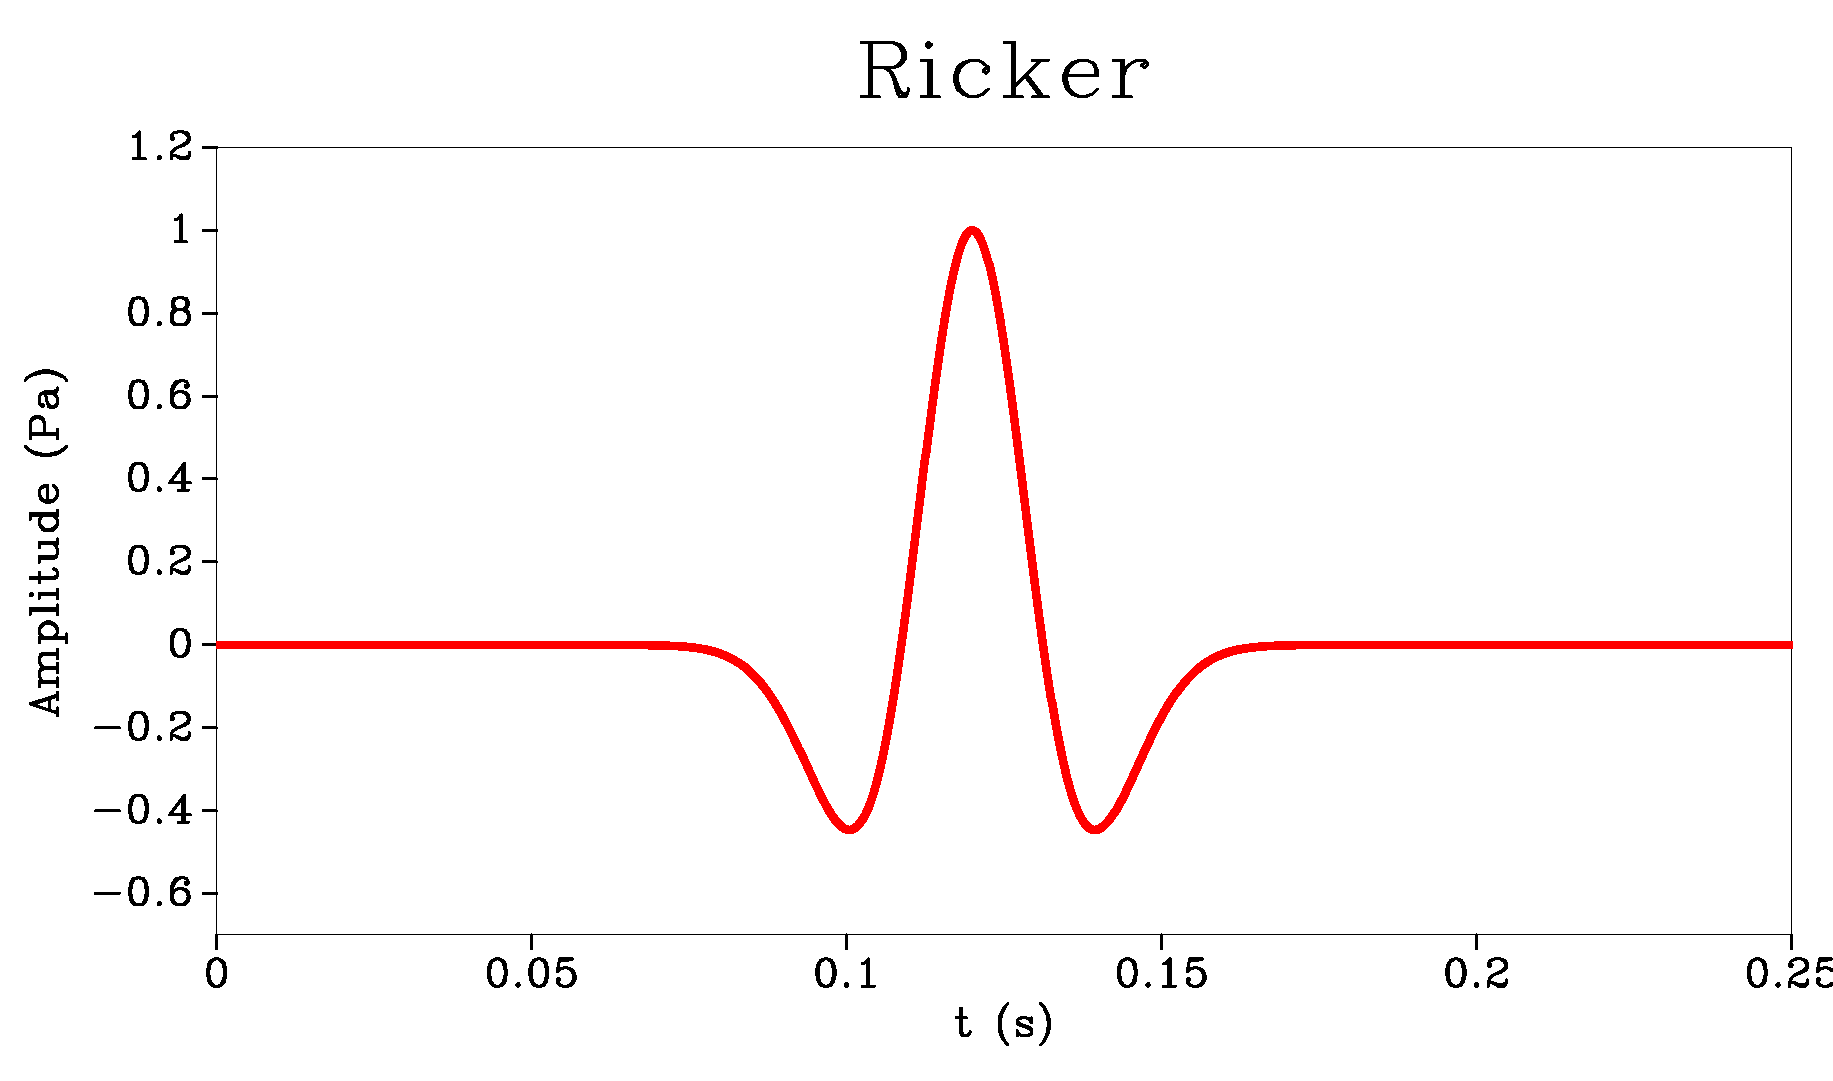
\includegraphics[width=15cm]{wav1}
	\caption{Assinatura da fonte usada: Ricker com frequência pico de $12~Hz$.} 
	\label{fig:ricker}
\end{figure} 

\section{M\'etodo das diferenças finitas}


Para encontrar a evolução do campo de onda, deve-se discretizar as equa\c{c}\~oes 
(\ref{eq.onda}). Esta será feita utilizando-se o método das diferenças 
finitas, que é caracterizado por substituir as derivadas de uma equação 
diferencial por expressões algébricas de diferenças. Essas expressões podem ser 
obtidas a partir do truncamento da expansão em série de Taylor e a ordem do erro 
da aproximação da derivada é função desse truncamento. 

A aplicação do método das diferenças finitas é realizada considerando o 
domínio discretizado em um \textit{grid} retangular de pontos, geralmente 
equiespaçados. Essa característica dificulta sua aplicação em domínios curvos. 
No entanto, este método possui uma boa acurácia e é de fácil implementação 
\citep{snieder1998}. Um problema é 
que o método não permite que se tenham \textit{grids} com refinamentos 
diferentes sobre o domínio \citep{zakaria2000two}. 


Esse método de discretização pode ser aplicado na 
equação da onda acústico vetorial.  Portanto, sabendo que é 
uma equação de primeira ordem, pode-se fazer a seguinte aproximaç\~ao centrada  para a 
derivada em rela\c{c}\~ao \`a $t$


\begin{equation}
\DDt[f(t)] \approx \frac{f(t+\Delta t)-f(t-\Delta t)}{2\Delta t} \label{eq:dif}
\end{equation} 
onde $f(t)$ é uma função qualquer e $\Delta t$ a diferença entre pontos consecutivos no tempo.
Para as outras diferenças finitas, progressiva e regressiva, tem-se as seguintes relações, respectivamente:
\begin{equation}
\DDt[f(t)] \approx \frac{f(t+\Delta t)-f(t)}{\Delta t} \label{eq:difp},
\end{equation}
\begin{equation}
\DDt[f(t)] \approx \frac{f(t)-f(t-\Delta t)}{\Delta t} \label{eq:difr},
\end{equation}

Para as equações (\ref{eq:dif}), (\ref{eq:difp}) e \ref{eq:difr}, foi utilizada a expansão da derivada de primeira ordem. Com o intuito de fazer a discretização em relação ao espaço, será substituído os termos $t$ e $\Delta t$ destas equações por $x$
e $\Delta x$. Sendo $x$ a variável espacial e o $\Delta x$ a diferença entre pontos consecutivos no espaço. 
\subsection{Cálculo dos coeficientes}
Para encontrar os coeficientes das diferenças finitas, foi utilizada a seguinte equação:
\begin{equation}
K\delta_{K,1}=2\sum_{j=0}^{N-1}d_j\Big(\frac{2j+1}{2}\Big)^K, \quad K=1, 3,...,2N \label{eq:coef}
\end{equation}
sendo que a solução deste sistema linear determina os coeficientes $d_j$ para uma aproximação de ordem 2N.
\section{Discretização da equação da onda}


Para encontrar a evolução do campo de onda, deve-se discretizar a equação 
(\ref{eq.onda}). Esta será feita utilizando-se o método das diferenças 
finitas. Portanto, sabendo que é 
uma equação de segunda ordem, pode-se fazer a seguinte aproximaç\~ao para a 
derivada parcial em rela\c{c}\~ao \`a $x$:
\begin{equation}
\frac{\partial^2P(x,z,t)}{\partial x^2}\approx\frac{P_{i+1,j}^{l}-2P_{i,j}^{l}+P_{i-1,j}^{l}}{\Delta x^2}, \label{dx2}
\end{equation}
onde $P_{i,j}^{l} = P(x_i,z_j,t_l)$ e $x_i = x_0 + i\Delta x$, $z_j = z_0 + 
j\Delta z$, e $t_l = t_0 + l\Delta t$. Esta \'e uma aproximação de segunda ordem. Pode-se, de maneira an\'aloga aproximar as segundas derivadas em $z$ e $t$.

Substituindo em (\ref{eq.onda}) as derivadas por suas aproxima\c{c}\~oes de diferen\c{c}as finitas e isolando o termo $P_{i,j}^{l+1}$, temos 
\begin{equation}
\begin{aligned}
P_{i,j}^{l+1}=c^2\frac{\Delta t^2}{\Delta h^2}(P_{i+1,j}^{l}+P_{i-1,j}^{l}+P_{i,j+1}^{l}+P_{i,j-1}^{l}-4P_{i,j}^{l}) \\
+ 2P_{i,j}^{l}-P_{i,j}^{l-1} - c^2 \Delta t S_{i,j}^l, \label{desenvol2}
\end{aligned}
\end{equation}

\section{Relação de dispersão}

Assumindo a propaga\c{c}\~ao de uma onda plana em um meio homog\^eneo, temos:
\begin{equation}
P_{i,j}^{l}=e^{i(k_{x}x_{i}+k_{z}z_{j}-\omega t_{l})}. \label{pij}
\end{equation}
A partir desta equação é possível determinar as seguintes relações:
\begin{eqnarray}
P_{i\pm1,j}^{l}&=&e^{i[k_{x}(x_{i}\pm\Delta x)+k_{z}z_{j}-\omega t_{l}]} \nonumber \\
&=&e^{\pm ik_{x}\Delta x}e^{i(k_{x}x_{i}+k_{z}z_{j}-\omega t_{l})} = e^{\pm ik_{x}\Delta x}P_{i,j}^{l}. \label{eq:Pi1}
\end{eqnarray}
De modo an\'alogo
\begin{equation}
P_{i,j\pm1}^{l}=e^{\pm ik_{z}\Delta x}P_{i,j}^{l}, \label{eq:Pj1}
\end{equation}
e 
\begin{equation}
P_{i,j}^{l\pm1}=e^{\mp i\omega\Delta t}P_{i,j}^{l}.\label{eq:Pt1}
\end{equation}
% \begin{equation}
% P_{i\pm1,j}^{l}=e^{\pm ik_{x}\Delta x}e^{i(k_{x}x_{i}+k_{z}z_{j}-\omega t_{l})} 
% \label{imp}
% \end{equation}
Substituindo as equações (\ref{eq:Pi1}), (\ref{eq:Pj1}) e (\ref{eq:Pt1}) em 
(\ref{desenvol2}), considerando $S_{i,j}^l=0$, tem-se que:
\begin{eqnarray}
e^{-i\omega\Delta t}P_{i,j}^{l}+e^{i\omega\Delta t}P_{i,j}^{l} 
&=&c^2\frac{\Delta t^2}{\Delta x^2}(e^{+ ik_{x}\Delta h
}P_{i,j}^{l}\\ \nonumber
& &+e^{- ik_{x}\Delta h}P_{i,j}^{l}+e^{+ik_{z}\Delta h}P_{i,j}^{l}\\ \nonumber
& &+e^{-ik_{z}\Delta h}P_{i,j}^{l}-4P_{i,j}^{l})+2P_{i,j}^{l}. 
\end{eqnarray}
A partir da relação de Euler para cosseno,
\begin{equation}
\cos(y)=\frac{e^{iy}+e^{-iy}}{2} \label{euller},
\end{equation}
podemos chegar na seguinte equação
% \begin{equation}
% 2\cos(y)=e^{iy}+e^{-iy} \label{euller2}.
% \end{equation}
% Substituindo a relação (\ref{euller2}) em (\ref{desen3}), podemos chegar na 
% seguinte equação:
% %Erro na numeração, n puxou o do eqnarray
\begin{equation}
\cos(\omega \Delta t) =c^2\frac{\Delta t^2}{\Delta h^2}(\cos(k_{x}\Delta h) + \cos(k_z\Delta h)-2) + 1.
\label{eq:disp1}
\end{equation}
Sendo $k = \frac{\omega}{c}$ o n\'umero de onda, podemos definir $k_x = k\sin \theta$ e $k_z = k \cos \theta$, onde $-\pi < \theta < \pi$ \'e a dire\c{c}\~ao de propaga\c{c}\~ao da onda plana em rela\c{c}\~ao ao eixo vertical, orientado para baixo. Com isso, Equação (\ref{eq:disp1}) fica
\begin{equation}
\cos(\omega \Delta t)=c^2\frac{\Delta t^2}{\Delta h^2}(\cos(k\sin \theta\Delta h) + \cos(k \cos\theta\Delta h)-2)+ 1.
\label{eq:disp2}
\end{equation}

Da eq. (\ref{eq:disp2}) podemos escrever 
\begin{eqnarray}
\omega (k,\theta)&=&\frac{1}{\Delta t} \cos^{-1}\Big\{ c^2\frac{\Delta t^2}{\Delta h^2}(\cos(k\sin \theta\Delta h) \nonumber\\ 
&&+ \cos(k \cos\theta\Delta h)-2)+ 1\Big\}.
\label{eq:disp3}
\end{eqnarray}
Desta equa\c{c}\~ao podemos escrever as express\~oes para velocidade de fase ($c_p$) e de grupo ($c_g$):
\begin{eqnarray}
c_p (f,\theta)\hspace{-8pt}&=&\hspace{-8pt}\frac{c}{2\pi f\Delta t} \cos^{-1}\Bigg\{ c^2\frac{\Delta t^2}{\Delta h^2}\left(\cos\left(\frac{2\pi f}{c}\sin \theta\Delta h\right)\right. \nonumber\\ 
&&+ \left.\cos\left(\frac{2\pi f}{c} \cos\theta\Delta h\right)-2\right)+ 1\Bigg\}
\label{eq:cp}
\end{eqnarray}
e
\begin{eqnarray}
c_g(f,\theta) &=& \Bigg(\frac{c^2\Delta t}{\Delta h} \left[ \sin(k\sin \theta\Delta h) \sin \theta \right. \nonumber \\ 
&& \left. + \sin(k\cos \theta\Delta h)\cos \theta\right]\Bigg) \times \nonumber \\
&& \Bigg(1 - \Big\{ c^2\frac{\Delta t^2}{\Delta h^2}(\cos(k\sin \theta\Delta h) \nonumber\\ 
&&+ \cos(k \cos\theta\Delta h)-2)+ 1\Big\}^2\Bigg)^{-1/2}.
\label{eq:cg}
\end{eqnarray}

A partir dessas equações, é possível gerar e ajustar gráficos com a velocidade de fase e de grupo, apresentados na Figura \ref{fig:disp}. 

\begin{figure}[ht!]
	\centering
	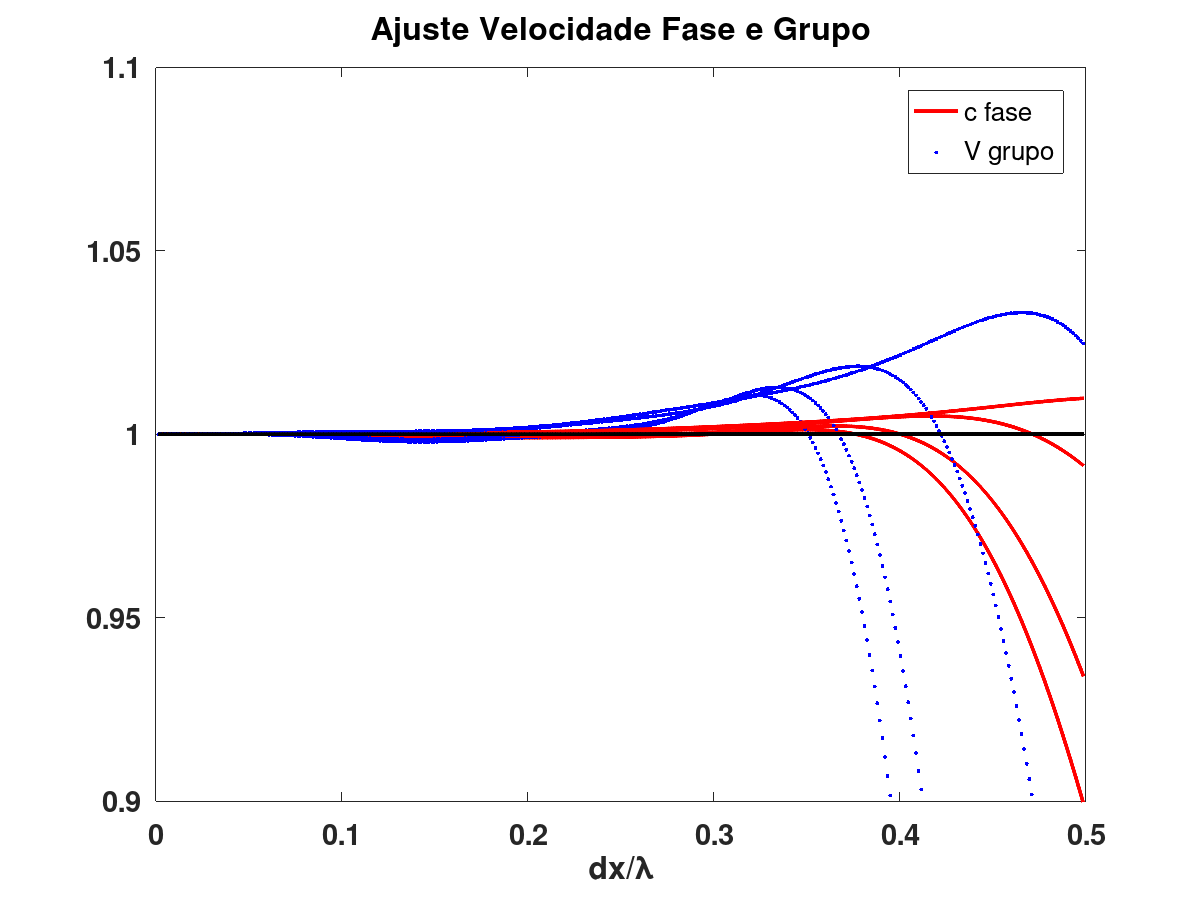
\includegraphics[width=11cm]{disper}
	\caption{Relação de dispersão, considerando ajustes na velocidade de fase e de grupo. Cada par de curvas está associado a um ângulo de propagação da onda plana.}
	\label{fig:disp}
\end{figure}

\section{Bordas de absorção}
Em uma solu\c{c}\~ao num\'erica, o meio de propaga\c{c}\~ao \'e finito. Assim, 
condi\c{c}\~oes de contorno devem ser aplicadas nas bordas do modelo. Estas causam, invariavelmente, reflex\~ao. 
Os dados que são refletidos pela borda ocasionam erros para os dados sísmicos
modelados, misturando o dado da propagação no meio com as reflex\~oes nas 
fronteiras do modelo. Com o intuito de retirar este efeito, deve ser aplicada 
uma borda absorvente, cujo objetivo é diminuir ou tirar a influência da 
reflexão das bordas \citep{komatitsch2007unsplit}.


\subsection{PML(Perfect Matched Layer)}

Com a finalidade de simular um meio ilimitado, \cite{berenger1994perfectly} introduziu a PML
(perfect Matched Layer), uma borda adicional em torno do meio limitado (Fig. \ref{fig:borda}) com amortecimento do campo de onda que chega nos limites
do modelo a fim de evitar as reflexões dos mesmos e, assim, interferir no sinal registrado. Na Figura \ref{fig:borda}, o $\sigma$ se refere ao amortecimento do campo de onda
que age apenas na região da borda.

\begin{figure}[ht!]
	\centering
	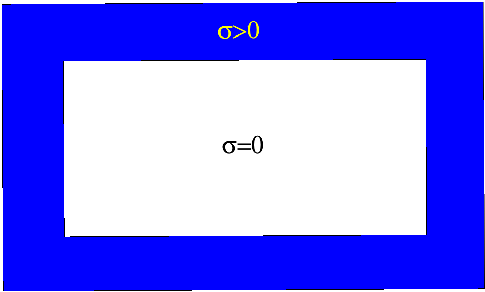
\includegraphics[width=11cm]{borda}
	\caption{Bordas adicionadas em volta de um modelo limitado para simular um meio
		ilimitado no processo de modelagem.}
	\label{fig:borda}
\end{figure}

Na Figura \ref{fig:borda}, o termo $\sigma$ pode ser definido da seguinte forma
\begin{equation}
\sigma(x)=\left\{\begin{matrix} 0 & \text{no dominío de interesse}  \\
\frac{3}{2}\text{log}(\frac{1}{R})c_{max}\Delta(\frac{x}{L}) & \text{nas bordas}, \\
\end{matrix}\right. \label{eq:sigma}
\end{equation}
sendo $R$ o coeficiente de reflexão desejado para incidência normal, $L$ a largura da banda de absorção e $f_{pico}$ a frequência pico do pulso.

Além de utilizar essa Equação \ref{eq:sigma},   tem-se uma implementação simples utilizando a seguinte equação:

\begin{equation}
\dddtt[p]+\sigma(x,y)\ddt[p]=c^2\nabla^2p, \label{eq:simples}
\end{equation}
sendo 
\begin{equation}
\sigma(x,y)=\lambda(x)+\lambda(y),
\end{equation}
com 
\begin{equation}
\lambda(x)=\left\{\begin{matrix} 0 & \text{no dominío de interesse}  \\
\pi f_{pico}\Delta (\frac{x}{L}) ^2& \text{nas bordas}, \\
\end{matrix}\right. \label{eq:lambda}
\end{equation}

A partir da Equação \ref{eq:simples}, pode-se reescrever \ref{desenvol2} da seguinte forma:
\begin{equation}
\begin{aligned}
p(x,z,t+\Delta)-2p(x,z,t)+p(x,z,t-\Delta)+\Delta\frac{\lambda(x)+\lambda(z)}{2}\{p(x,y,t+\Delta) \\
-p(x,y,t-\Delta)\}\\
=\Big{(}\frac{c(x,z)\Delta}{h}\Big{)}^2\{2d_0p(x,z,t) \\
+ \sum_{j=1}^{N-1}d_j(p(x+jh,z,t)+p(x-jh,z,t))\\
+ \sum_{j=1}^{N-1}d_j(p(x,z+jh,t)+p(x,z-jh,t))\} \\
+\Delta t^2S(t)\delta_{BL}(\vc{x}-\vc{x_s})+O(\Delta t^2,h^{2N})
\end{aligned}
\end{equation}

\section{RTM}
 
A técnica da Migração Reversa no Tempo consiste em propagar o sinal do tempo final para o tempo inicial, na qual é aplicada uma
condição de imagem para obter a imagem em profundidade. Essa técnica de imageamento vantagens quando comparado com outras
técnicas por solucionar a equação de onda completa da onda e viabilizar o imageamento de
estruturas mais complexas \citep{matias}.

\begin{equation}
	I(\vc{x})=\sum_{s}\int_{0}^{T}\sum_{r}p_s(\vc{x},t;\vc{x}_S)p_r(\vc{x},t;\vc{x}_r)dt,
\end{equation}
na qual $I(\vc{x})$ é a imagem final migrada para cada ponto, $\vc{x}_S$ é a posição da fonte, $\vc{x}_r$ é a posição do receptor, $T$ é o tempo total de registro, $p_s$ o campo de onda que inicia na fonte e $p_r$ o retropropagado pelos receptores.

\section{Paralelização}

É necessário frequentemente utilizar diversas unidades de processamento para obter o poder computacional desejado para resolver alguns problemas. A fim de atender a essa demanda, foram criados sistemas que possuem essas diversas unidades de processamento, objetivando aumentar a capacidade de computação ao menor custo possível. A um sistema com diversas dessas unidades se dá o nome de \textit{cluster}. Cada um dos processadores de um \textit{cluster} é chamado de nó.

Paralelizar um processamento de dados é dividir o esforço computacional entre diversos processadores e fazer com que isso ocorra de forma aproximadamente simultânea \citep{chandra2001parallel}. A paralelização pode ser implementada através de uma divisão do bloco inicial de dados em blocos menores que podem ser processados individualmente, simultaneamente e em menos tempo do que o bloco inicial. Ao final, os dados oriundos dos diversos processamentos devem ser agregados para se obter o resultado final. Uma paralelização pode ser implementada e executada num sistema paralelo ou em um sistema distribuído. 

As complicações referentes a paralelização podem ocorrer devido a divisão de trabalho entre os processadores, garantir que os passos sequenciais estejam sendo executados de forma correta e garantir exclusão mútua no acesso aos recursos. Para resolver esses problemas, a forma é garantir a sincronização dos processos envolvidos. 


\chapter{FILTRAGEM F-K}
\label{cap3}

A transformada de Fourier (TF) constitui um dos maiores produtos da física e da matemática, e é indispensável na teoria e no processamento de sinais por várias razões. 
Uma das primeiras é que a sua base é estruturada no conceito de \textit{frequência}, o que permite uma compreensão melhor do fenômeno sendo estudado, e que adiciona um complemento ao sinal temporal (espacial) que é inicialmente usado para análise. 
Esta condição é muito comum, e os exemplos são vários na física de ondas (como na acústica, sísmica, eletromagnetismo, vibrações, ótica, etc.), bem como em outras áreas onde processos periódicos são importantes e regem os fenômenos de interesse (como na biomedicina, biologia, astronomia, economia, etc.). \cite{Lourenildo(2015)}

Para tornar a descrição mais prática, define-se o par das integrais direta, $G(\omega)$, e inversa, $g(t)$, em 1D nas seguintes formas ilimitadas (o que se faz para um lado $t,\omega \rightarrow +\infty$ se faz para o outro $t,\omega \rightarrow -\infty$):
\begin{equation}
G(\omega)=k_{1}\int_{-\infty}^{\infty}g(t)e^{-i\omega t}dt, \quad G(\omega)=F\{g(t)\}, \quad (i=\sqrt{-1}),
\label{eq.3.1}
\end{equation}
\begin{equation}
g(t)=k_{2}\int_{-\infty}^{\infty}G(\omega)e^{+i\omega t}d\omega, \quad g(t)=F^{-1}\{G(\omega)\}, \quad (\omega=2\pi f).
\label{eq.3.2}
\end{equation}
A escolha dos coeficientes $k_{1}$ e $k_{2}$ dependem do usuário ou do problema em estudo. O requerimento é que o produto $k_{1}k_{2}=1/2\pi$. Se $k_{1}=k_{2}$, então, $k_{1}=1/\sqrt{2\pi}$. Se $k_{1}=1$, então, $k_{2}=1/2\pi$.

Para o caso 2D, temos a TF direta na forma da equação (\ref{eq.3.3}) e TF inversa na equação (\ref{eq.3.4})

\begin{equation}
h(t, x)=\int_{-\infty}^{\infty} \int_{-\infty}^{\infty} H(f_{t}, f_{x}) e^{+i 2 \pi(f_{t} t+f_{x} x)} df_{t} df_{x}
\label{eq.3.3}
\end{equation}
\begin{equation}
H(f_{t}, f_{x})=\int_{-\infty}^{\infty} \int_{-\infty}^{\infty} h(t, x) e^{-i 2 \pi(f_{t} t+f_{x} x)} dt dx
\label{eq.3.4}
\end{equation}

Para estas equações se tem as relações: $f_{t}=\frac{1}{T} $, $f_{x}=\frac{1}{\lambda}=\frac{1}{vT}$, de onde se estabelece a relação $f_{t}=vf_{x}$; isto é, nestas condições a frequência temporal, $f_{t}$, e a frequência espacial, $f_{x}$, são acopladas através de uma relação linear $f_{t}=vf_{x}$, onde $v$ é o parâmetro de inclinação.
Também, usando a vagarosidade $s=\frac{1}{v}$ se tem a forma $f_{x}=sf_{t}$. 
A figura \ref{fig:Relacao_Dispersao} mostra a relação entre estas quantidades, com a descrição da propagação de uma onda plana, e a relação denominada de dispersão que envolve as frequências espaciais e a temporal.

\begin{figure}[H]
\centering
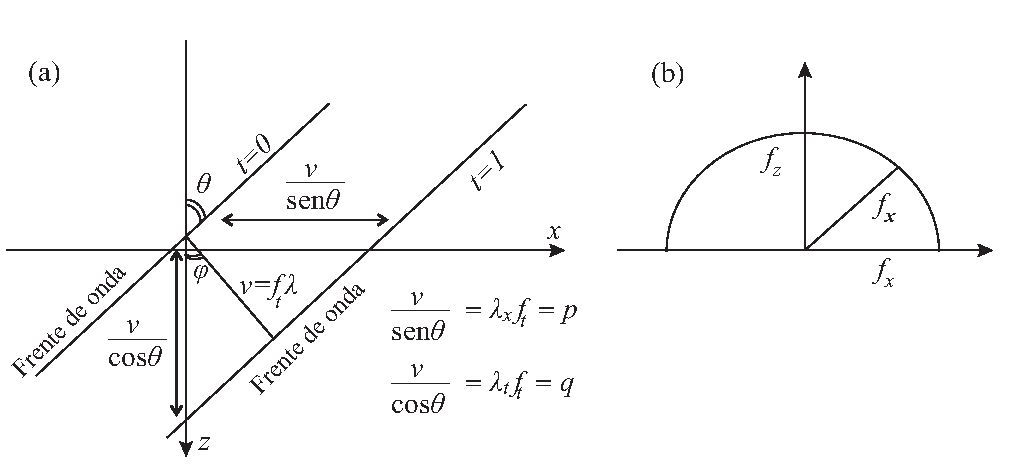
\includegraphics[width=12cm]{figuras/cap3/Relacao_Dispersao.pdf}
\vspace{-0.3cm}
\caption{Descrição física da relação entre a frente de onda e a equação da dispersão. 
(a) Propagação da onda plana. 
(b) Relação entre as componentes $f_{x}$ e $f_{z}$ e a total $f_{\mathbf{x}}$ para $f_{t}$ constante.}
\label{fig:Relacao_Dispersao}
\end{figure}

\section{Filtros de corte na frequência}

O princípio a ser aplicado é o de que os eventos possam ser separados no domínio da frequência, $f_{t}-f_{\mathbf{x}}$, de alguma forma, pelo menos parcial.  
Partindo deste princípio, a figura \ref{fig:Analise_Idealizada_Sinal_Ruido_Frequencia} ilustra a composição espectral, e serve para a análise da relação frequência temporal-espacial (número de onda) do conteúdo de velocidades comumente presente em experimentos de sísmica de exploração.

\begin{figure}[H]
\centering
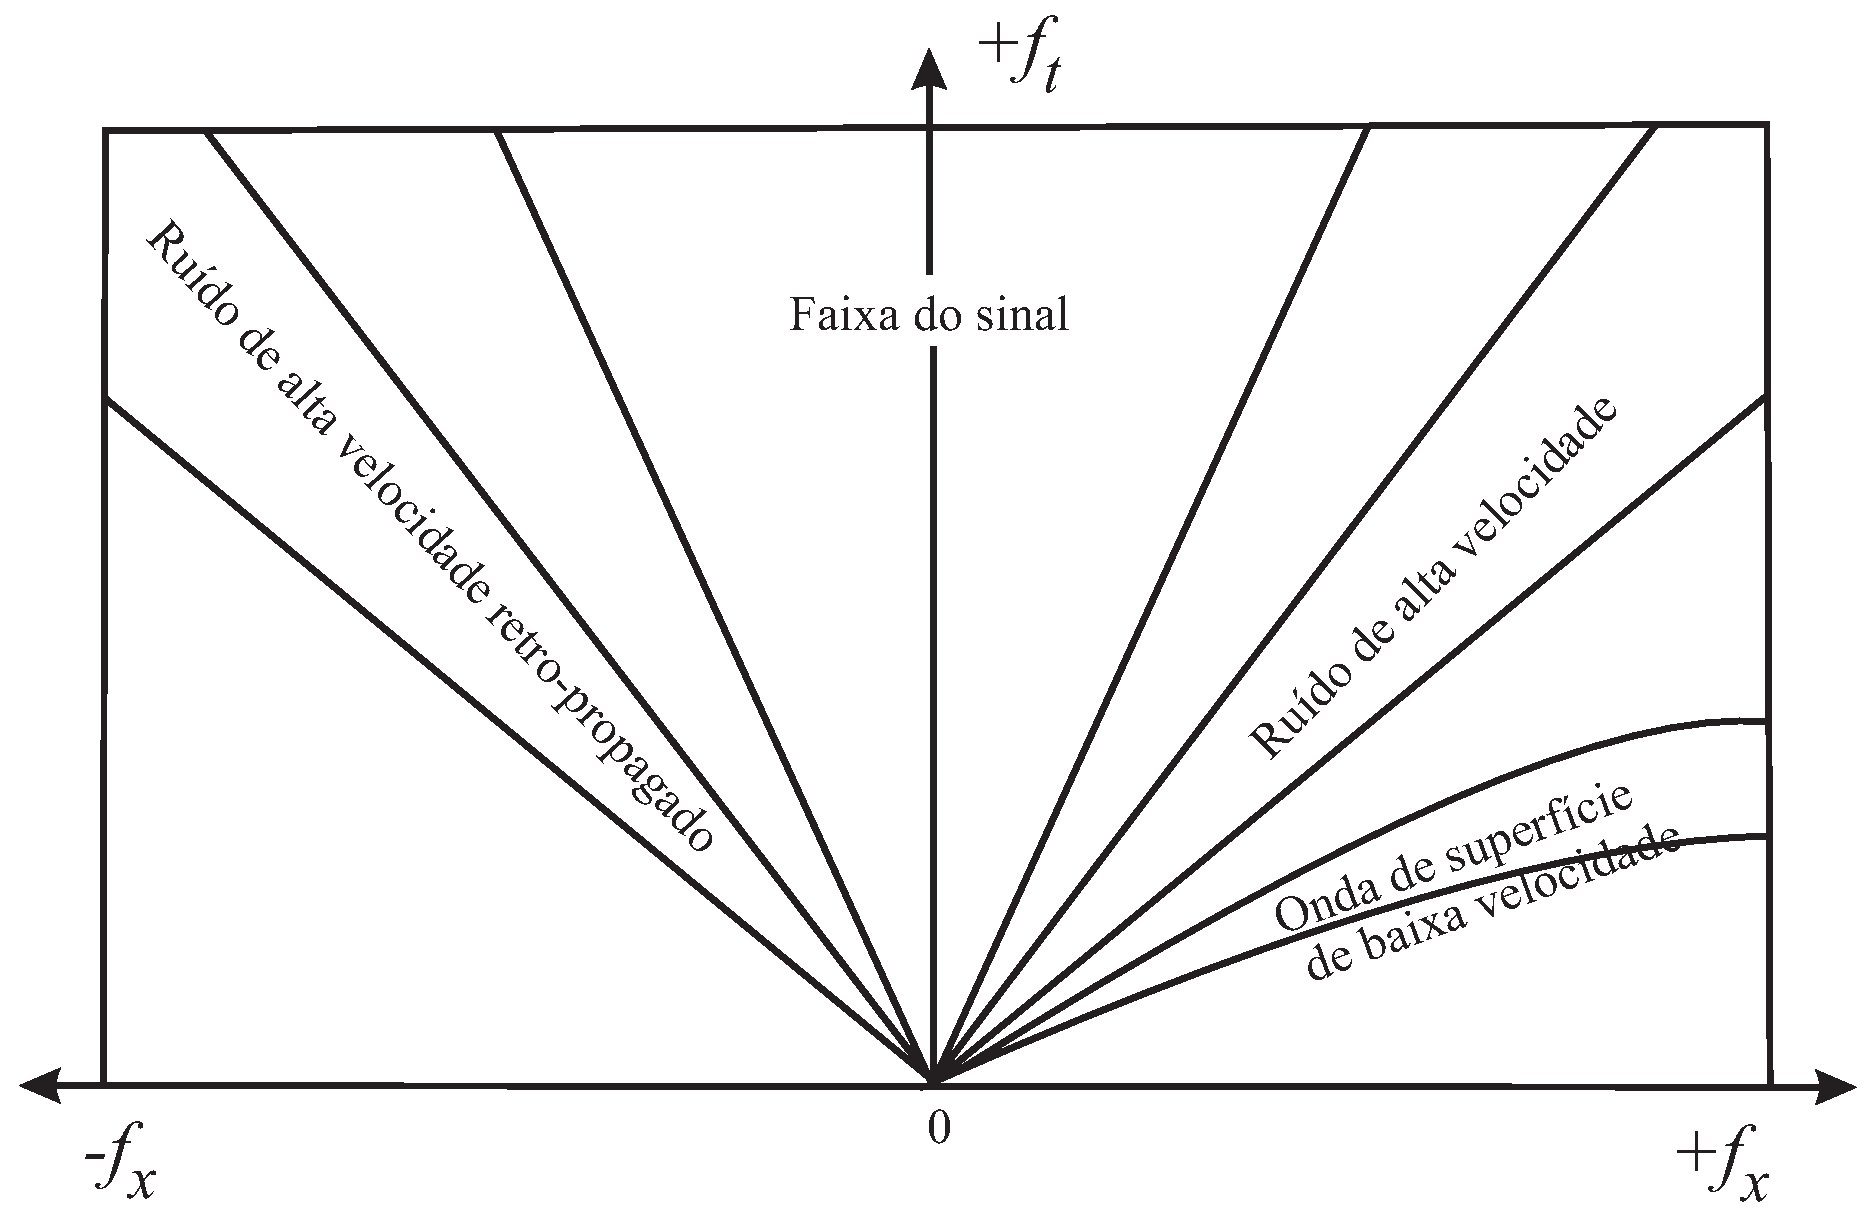
\includegraphics[width=11cm]{figuras/cap3/Analise_Idealizada_Sinal_Ruido_Frequencia.pdf}
\vspace{-0.3cm}
\caption{Ilustração da composição espectral de uma seção sísmica (frequência temporal-espacial). 
Se destacam as linhas de sinal de informação, ruídos de velocidade alta e baixa, e ruido das ondas de superfície de baixa frequência. As linhas inclinadas separam os eventos mergulhantes no domínio $f_{t}-f_{\mathbf{x}}$.}
\label{fig:Analise_Idealizada_Sinal_Ruido_Frequencia}
\end{figure}

A figura \ref{fig:Analise_Idealizada_Filtro_Separa} ilustra o problema que se encontra na tentativa de se aplicar um filtro, $H(f_{t},f_{x})$, convencional simples, o que se ilustra com a figura \ref{fig:Filtro_velocidade}, que tem por finalidade esboçar a relação linear simples (outra forma qualquer pode ser desenhada) no domínio espectral para o caso prático de dados no domínio do discretizado; as frequências de Nyquist estão definidas: 
$f_{Nt}=\frac{1}{2 \Delta t}$, $f_{Nx}=\frac{1}{2 \Delta x}$ e $f_{Nt}= vf_{Nx} =\frac{v}{2 \Delta x}$.
Neste caso, $v$ é a velocidade e $s$ é a vagarosidade.
Observe-se na figura \ref{fig:Filtro_velocidade} as faixas de passagem e de rejeição lineares, onde está superposto uma ilustração de uma linha de contorno típica (forma qualquer) do espectro de um dado real. 
A relação entre as linhas de corte (passagem-rejeição) linear e espectro real não é simples, o que se deseja é que as linha sejam o mais alinhado (paralelo) possível.
%=====================================================
\begin{figure}[H]
\centering
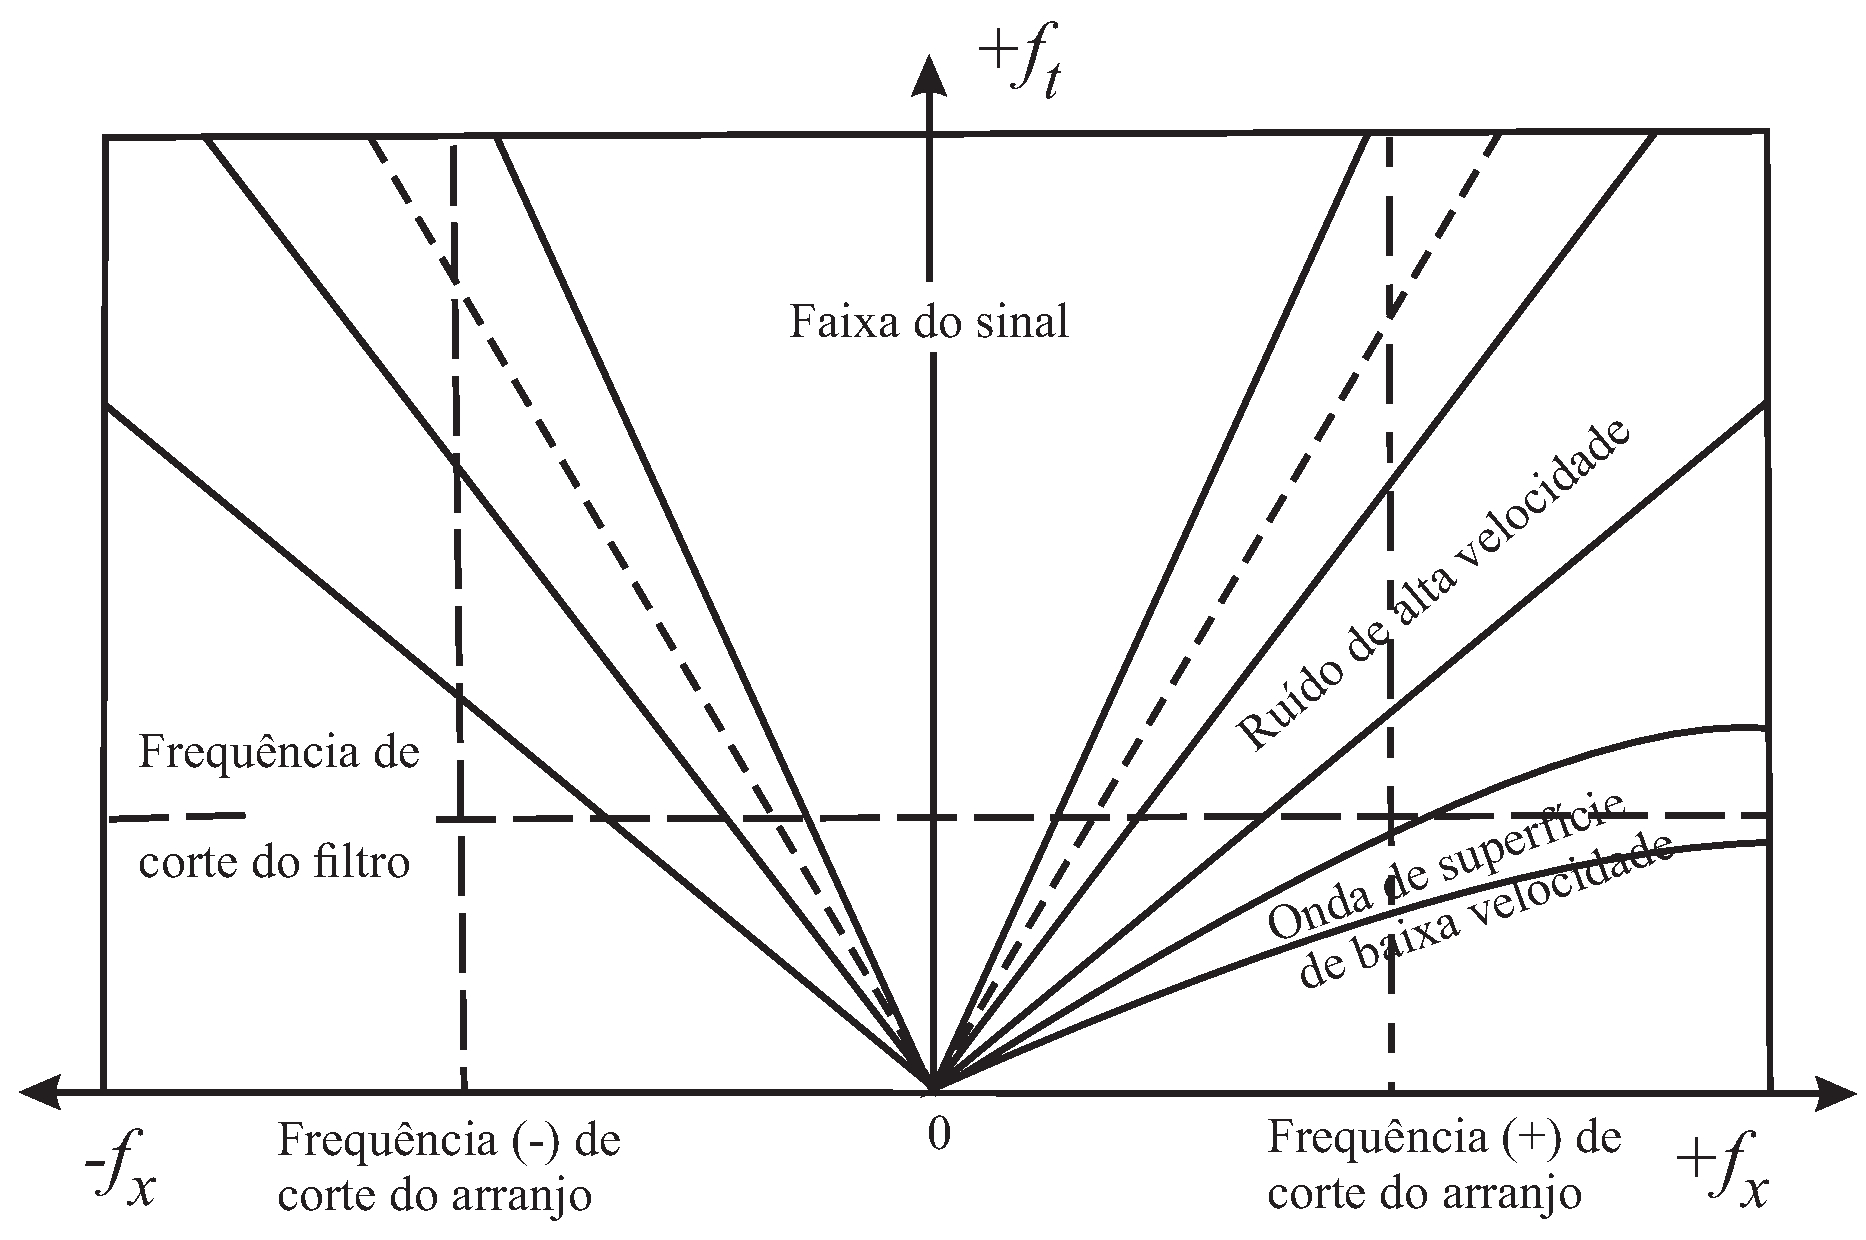
\includegraphics[width=11cm]{figuras/cap3/Analise_Idealizada_Filtro_Separa.pdf}
\vspace{-0.3cm}
\caption{Construção idealizada do filtro para separação da composição espectral de uma seção sísmica (frequência temporal-espacial) correspondente à figura \ref{fig:Analise_Idealizada_Sinal_Ruido_Frequencia}. 
Se destacam as linhas de sinal de informação, ruídos de velocidade alta e baixa, e ruido das ondas de superfície de baixa frequência.}
\label{fig:Analise_Idealizada_Filtro_Separa}
\end{figure}
%=====================================================
%=======================================================
\begin{figure}[H]
\centering
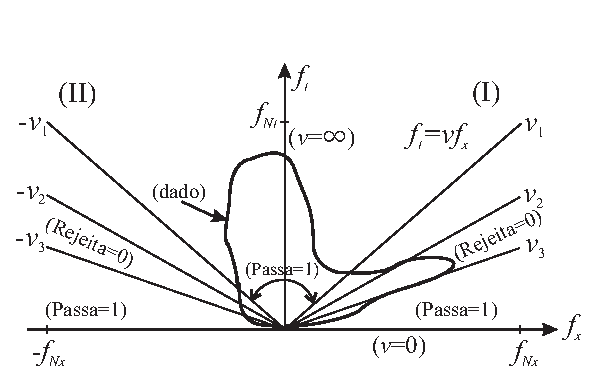
\includegraphics[width=12cm]{figuras/cap3/Filtro_velocidade.pdf}
\vspace{-0.3cm}
\caption{Divisão do domínio da frequência 2D em quadrantes, ilustração do espectro de (dado) real, $H_{R}(f_{t},f_{x})$, e desenho do filtro com a forma Em-leque de Passagem-Rejeição (EL-P-R). 
Para completar o filtro é necessário refletir os quadrantes: I para III e II para IV.}
\label{fig:Filtro_velocidade}
\end{figure}
%=======================================================

A figura \ref{fig:Analise_Idealizada_Filtro_Separa} esboça a tentativa de se preservar uma banda de frequências mais ampla possível. 
Para isto se analisa a geometria do arranjo de registro (padrão de distribuição dos sensores nas estações, padrão de tiro, etc.), e ao passo que as dimensões geométricas do arranjo aumenta, a linha de corte vai no sentido de $f_{x}$ menor (comprimento de onda maior). 
Ao passo que as dimensões do arranjo aumenta, o sistema atenua a informação de eventos de mergulho (linear) e ruído.
E se as dimensões continuam aumentando, o corte passa para o leque do sinal de informação (Faixa do sinal).

\section{FILTRAGEM F-K DA SEÇÃO TIRO 50}

Após a aquisição do dado sísmico figura (\ref{fig:afastamento_min}) no $SU$ com a subrotina \textit{triseis} utilizou-se o tiro $50$ para a filtragem F-K no \textit{matlab}, onde foi implementado os plots da seção tiro figuras (\ref{fig:tiro_50}), (\ref{fig:tiro_50gain}), (\ref{fig:tiro_50ruido}) e (\ref{fig:tiro_50ruido_gain}). 

O ruído é intrínseco ao registro do traço sísmico, seja como consequência do meio geológico ou do próprio equipamento de registro utilizado. Para simular a entrada de ruído na seção sísmica, assumimos o pressuposto de que ele equivale a um arranjo de números aleatórios de média zero.

\begin{figure}[H]
\centering
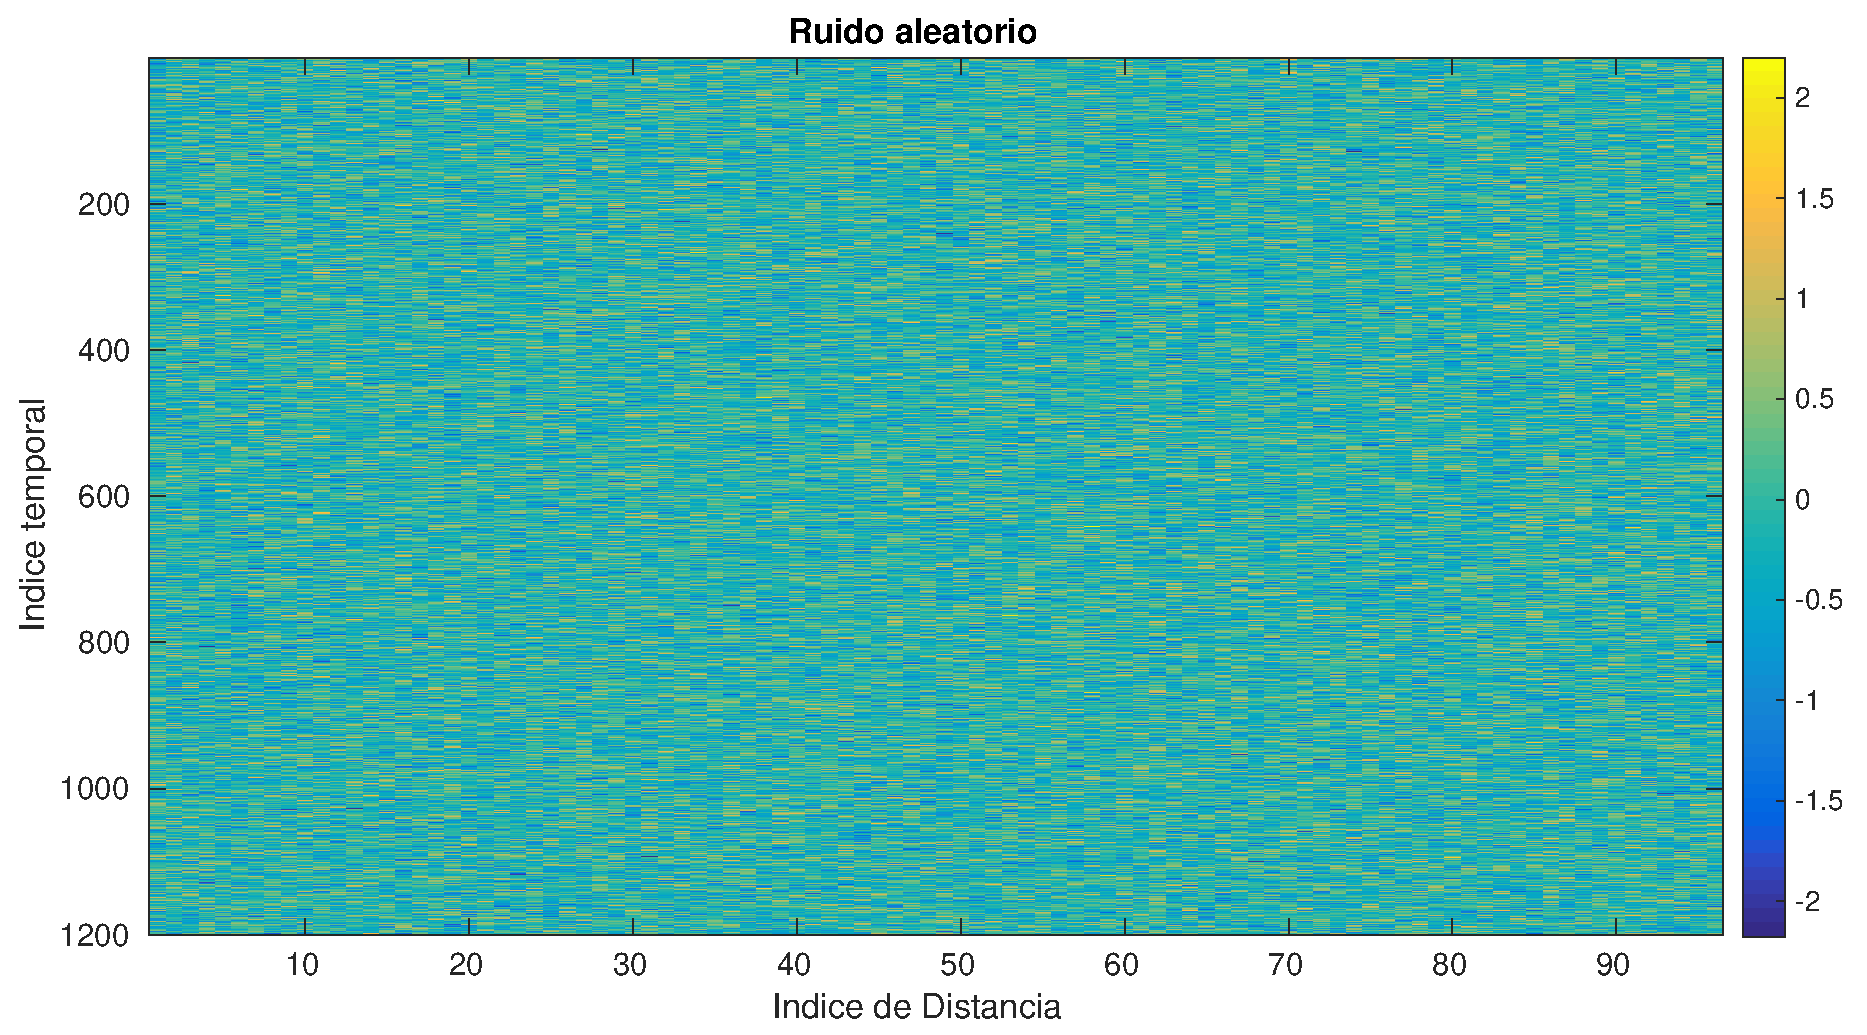
\includegraphics[totalheight=7.0cm]{figuras/cap3/ruido_aletorio.eps}
\caption{Ruído aleatório gerado no matlab}
\label{fig:ruido_aletorio}
\end{figure}

Nas seções sísmicas se precisa aplicar uma função de ganho devido à diminuição da amplitude com a distância-tempo, denominado de  espalhamento geométrico, divergência esférica, e às vezes atenuação tempo-distância. 
A função ganho empregada corresponde a uma amplificação do sinal no tempo para que se possa ver e interpretar a composição do sinal, que na sísmica é composto de eventos do tipo ruído, reflexões, refrações, múltiplas e difrações. 
Isto é, a correção de espalhamento geométrico por uma função ganho é aplicada para compensar o decaimento de energia da divergência da frente de onda em qualquer fase do processamento de uma seção sísmica. 
Ressalta-se que a aplicação de um ganho é uma operação destrutiva, ou não-destrutiva; o ganho aplicado é classificada como quase não-destrutivo devido ao ponto zero anulado.
A função ganho aplicada é dada por 

\begin{equation}
g(t)=t^{a}e^{-bt},
\label{eq:figura_ganho}
\end{equation}

onde os valores utilizados para os parâmetros foram $a=2$ e $b=0,5$.

\begin{figure}[H]
\centering
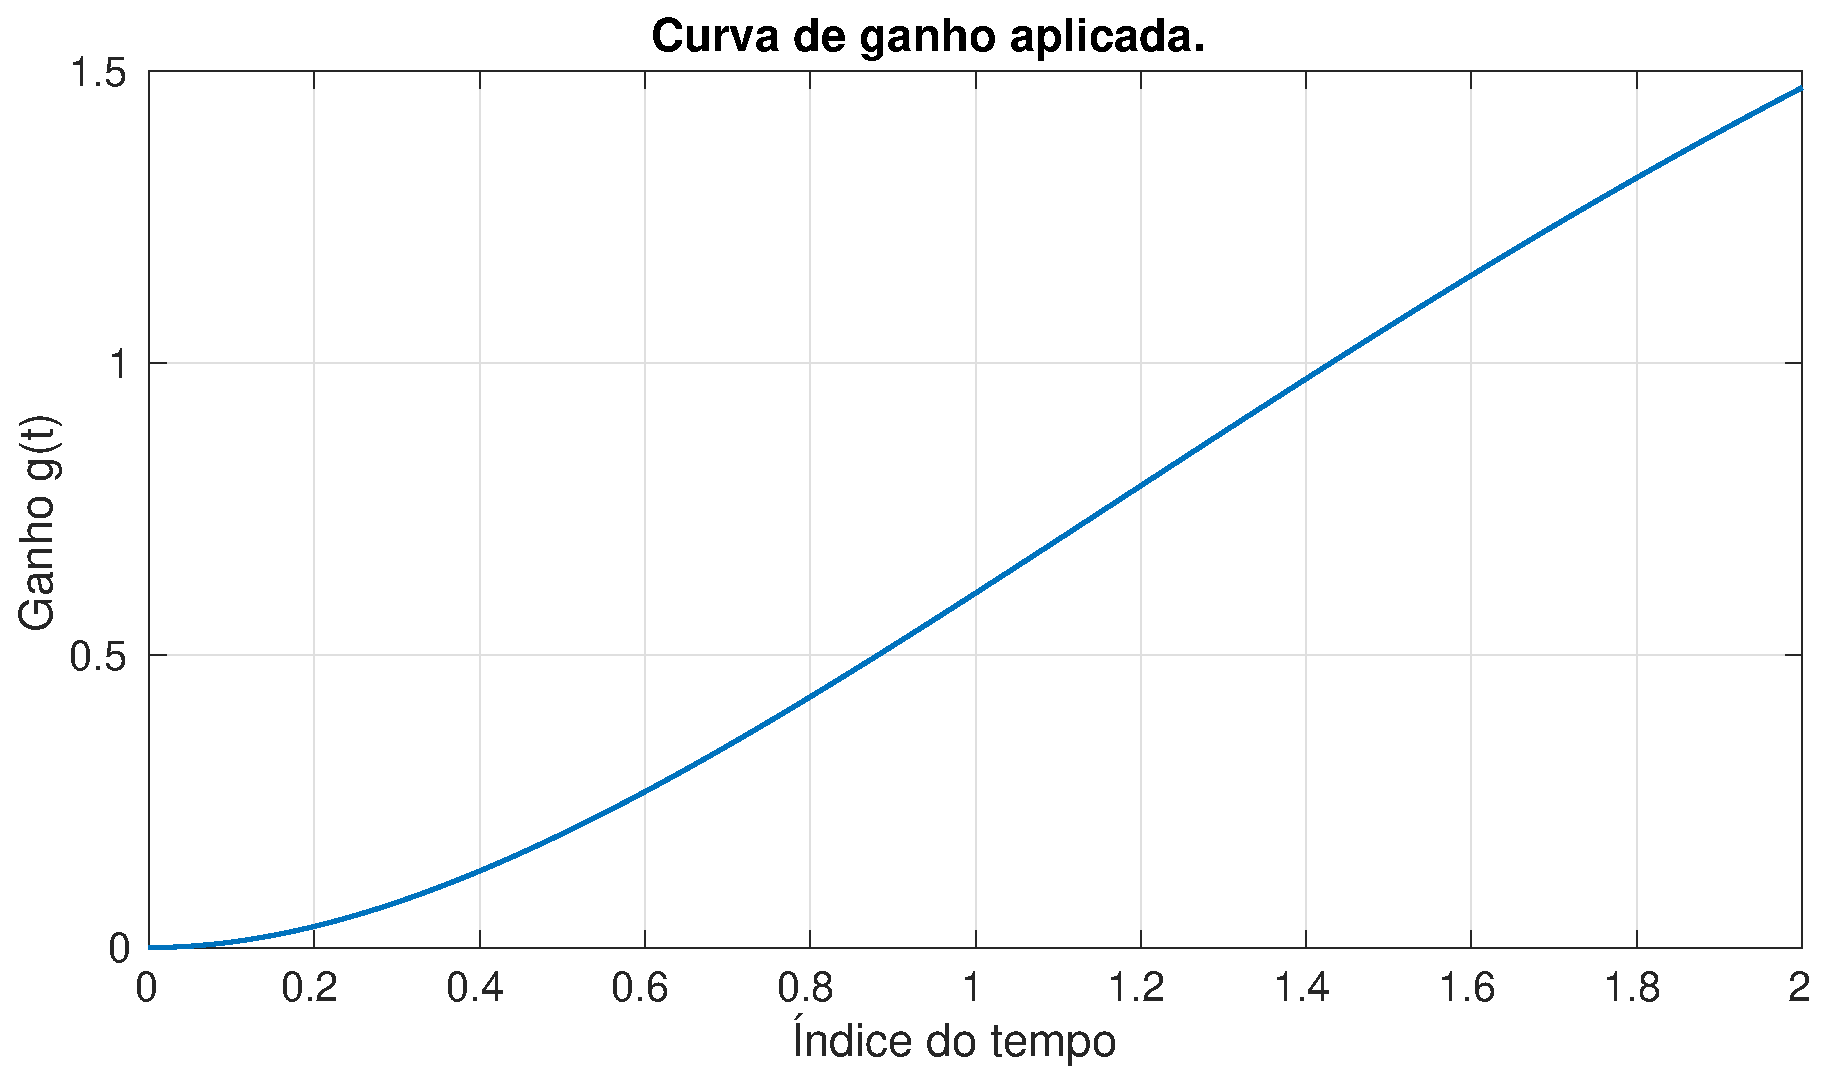
\includegraphics[totalheight=7.0cm]{figuras/cap3/figura_ganho.eps}
\caption{Função ganho empregada.}
\label{fig:figura_ganho}
\end{figure}

A figura \ref{fig:figura_ganho} mostra a variação do ganho, onde se observa que ela é crescente, mas com um intervalo de amplificação entre zero e $1,5$, que se apresenta de uma forma diferente, mas consistente no que se refere a colocar os valores num intervalo menor.  

Para que se possa realizar uma filtragem, a informação a ser recuperada deve ser separável do não-desejado, no domínio-f , ou no domínio-t.

A figura (\ref{fig:espc_tiro50}) mostra o espectro de amplitude da seção tiro 50 com ruído gerada a partir da figura (\ref{fig:tiro_50ruido}).

O termo filtro é reservado para a operação de multiplicação no domínio da frequência, e pode zerar a parte não desejada do espectro do sinal. Através da definição do espectro de amplitude e de fase podemos construir o operador $H(f)=A(f)e^{\theta(f)}$, que representa o filtro na frequência. Todo e qualquer processo de filtragem de um sinal pode ser representado na seguinte forma:

\begin{equation}
S_{H}(f)=G(f) H(f)
\label{eq:filtragem}
\end{equation}

Onde $S_{H}$ representa o sinal filtrado no domínio da frequência, $G(f)$ representa o sinal a ser filtrado e $H(f)$ o filtro a ser aplicado. Ou no domínio tempo na forma de convolução:

\begin{equation}
s_{h}(t)=s(t) \ast h(t)
\label{eq:filtragem_conv}
\end{equation}

As figuras (\ref{fig:espc_tiro50_c1}), (\ref{fig:espc_tiro50_c2}) e (\ref{fig:espc_tiro50_c3}) ilustram a geometria de passagem e rejeição de uma forma geral.

Após a filtragem da seção tiro 50 (ver figura \ref{fig:secao_filtrada}) nota-se que a maior parte da componente de ruído (informação não desejável) foi removida com a filtragem F-K. O corte no espectro de amplitude de maneira iterativa pelo matlab permite maior precisão na eliminação do ruído. Comparando a figura (\ref{fig:secao_filtrada}) com (\ref{fig:tiro_50ruido}), respectivamente a seção tiro 50 filtrada sem ganho e seção tiro 50 com ruído.

Em seguida a figura (\ref{fig:secao_filtrada_gain}) mostra a atuação do ganho na seção tiro 50 filtrada, o ganho aumenta com o tempo ou seja não apenas os eventos desejavéis são amplificados como também a componente de ruído. Comparando as duas figuras (\ref{fig:secao_filtrada_gain}) com (\ref{fig:tiro_50ruido_gain}) onde respectivamente representam a seção tiro 50 filtrada com ganho e seção tiro 50 com ruído e ganho. 

\begin{landscape}
\begin{figure}[H]
\centering
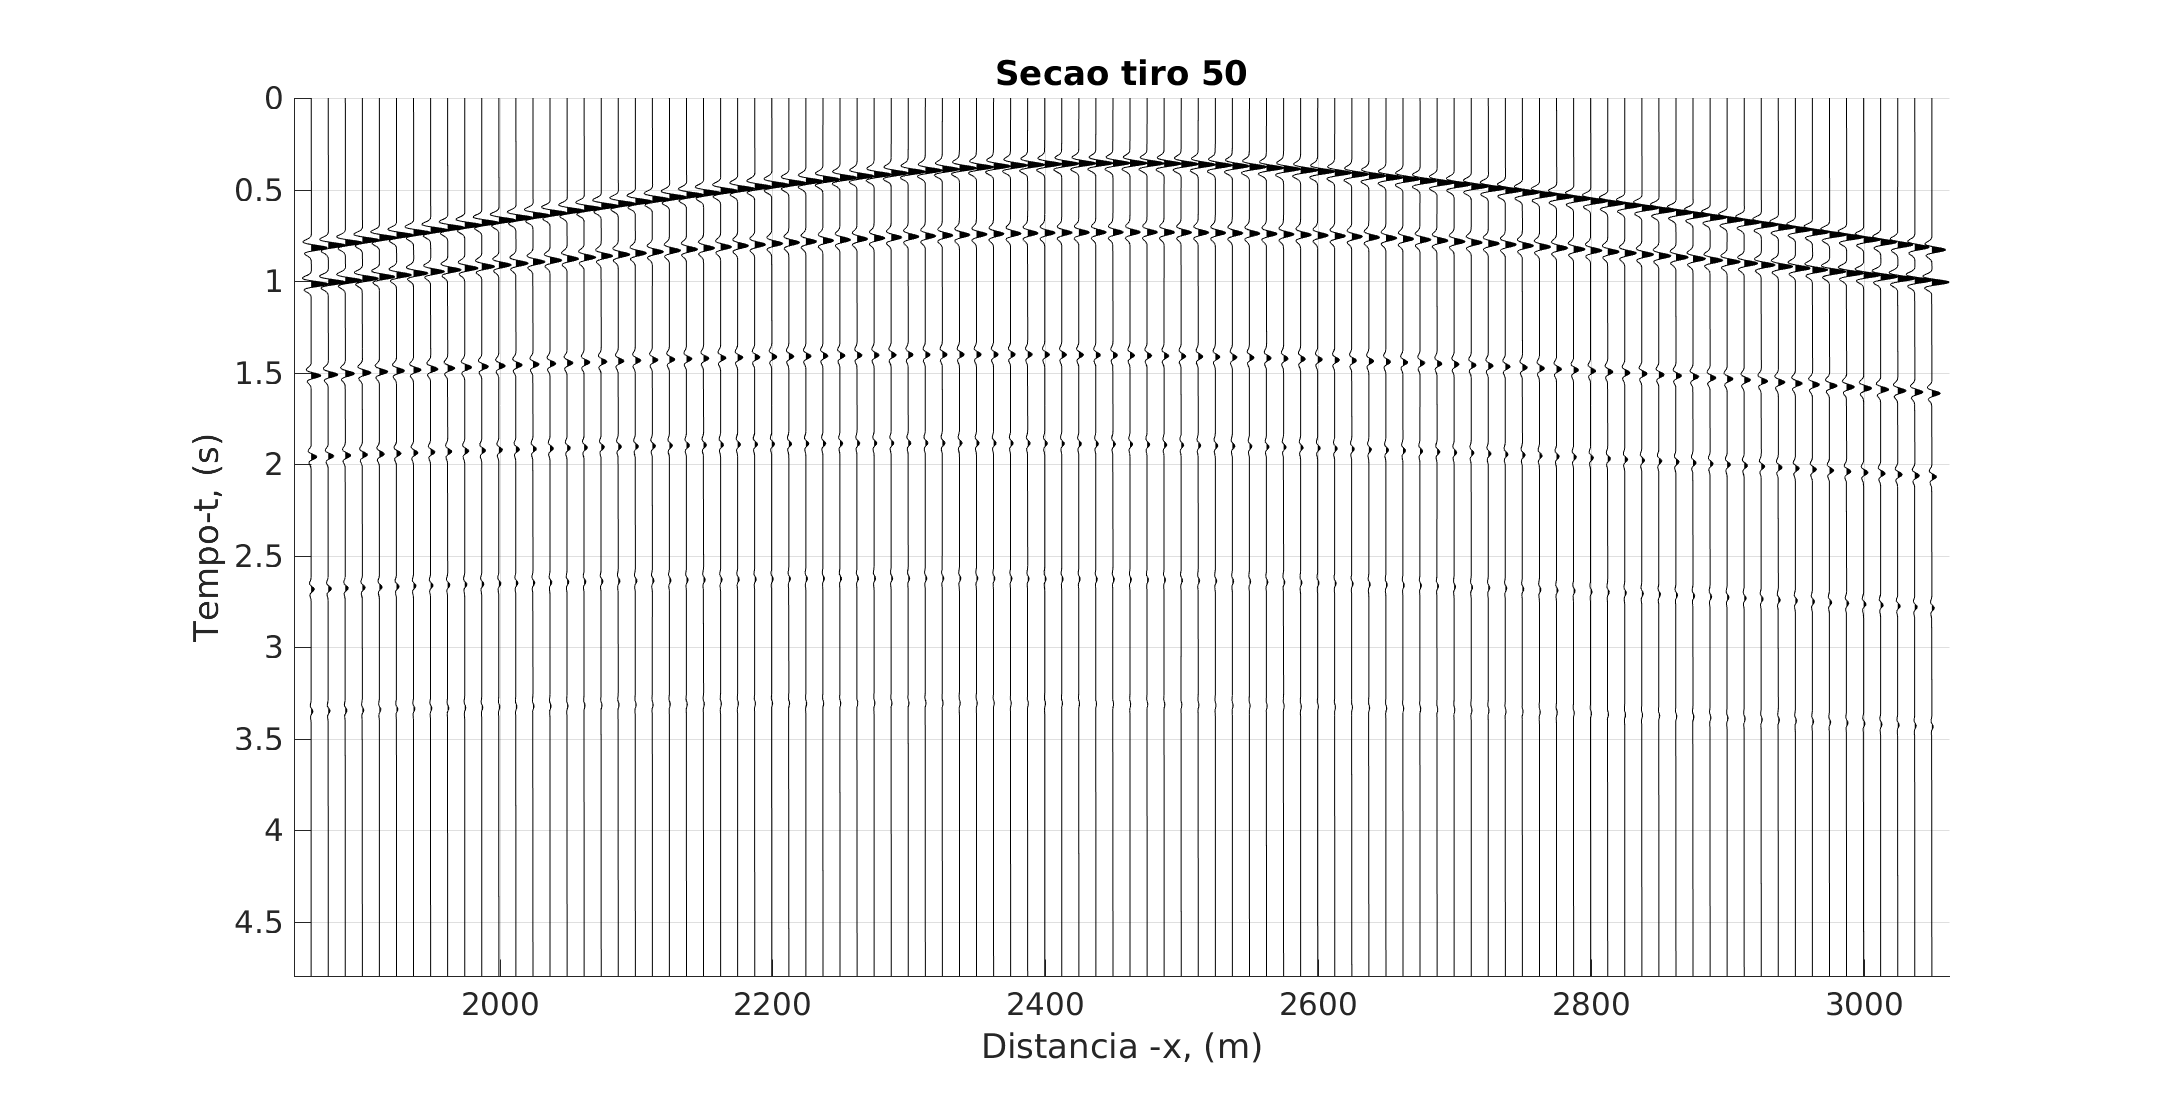
\includegraphics[totalheight=14cm]{figuras/cap3/secao_tiro50.eps}
\caption{Seção tiro 50 sem ganho do modelo sintético, figura (\ref{fig:vagarosidade})}
\label{fig:tiro_50}
\end{figure}
\end{landscape}

\begin{landscape}
\begin{figure}[H]
\centering
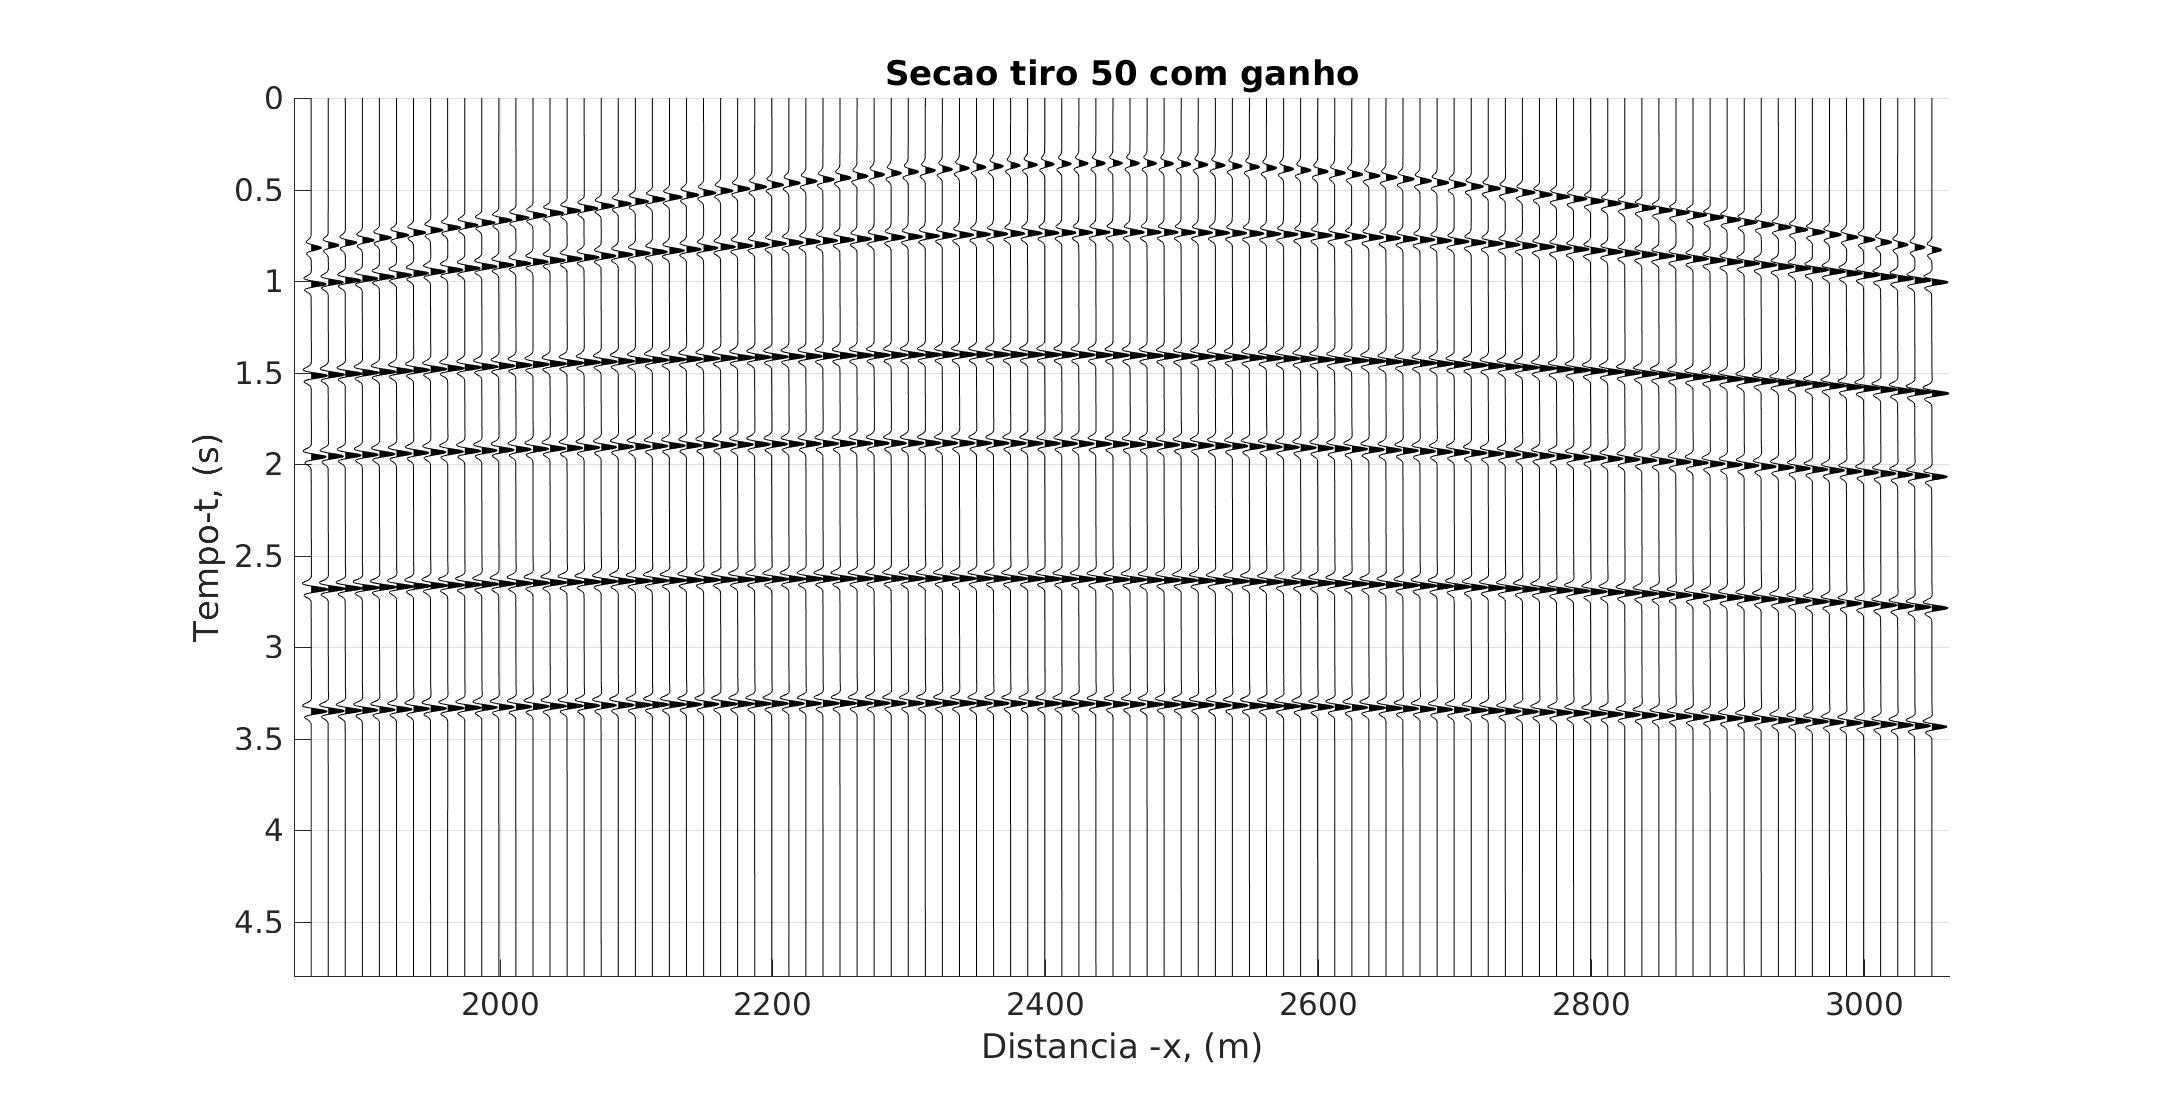
\includegraphics[totalheight=14cm]{figuras/cap3/secao_tiro50_ganho.eps}
\caption{Seção tiro 50 com ganho, os eventos com maior tempo foram realçados.}
\label{fig:tiro_50gain}
\end{figure}
\end{landscape}

\begin{landscape}
\begin{figure}[H]
\centering
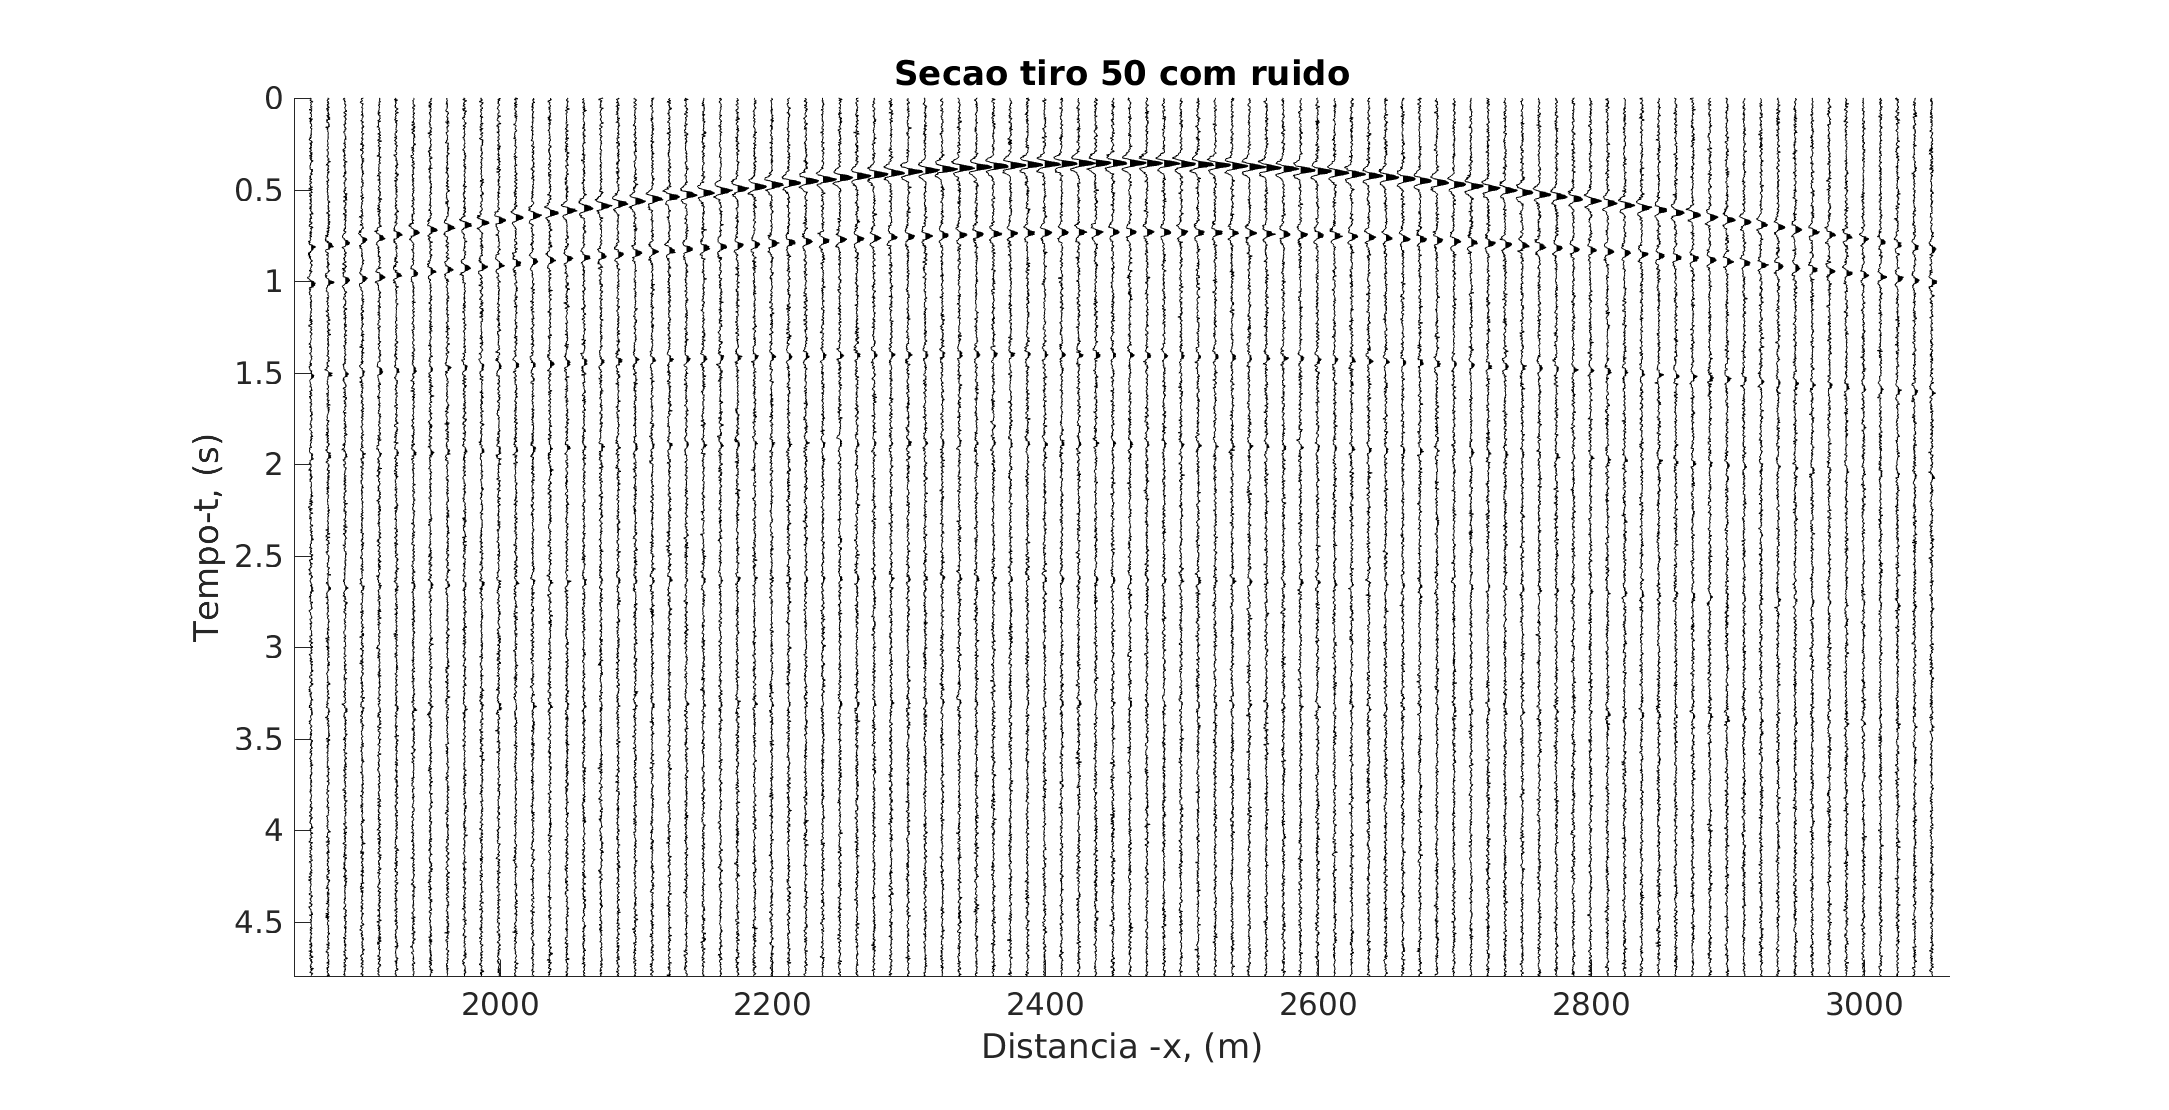
\includegraphics[totalheight=14cm]{figuras/cap3/secao_tiro50_ruido.eps}
\caption{Seção tiro 50 com ruido aleatório, o ruído foi gerado no matlab e somado a seção tiro 50.}
\label{fig:tiro_50ruido}
\end{figure}
\end{landscape}

\begin{landscape}
\begin{figure}[H]
\centering
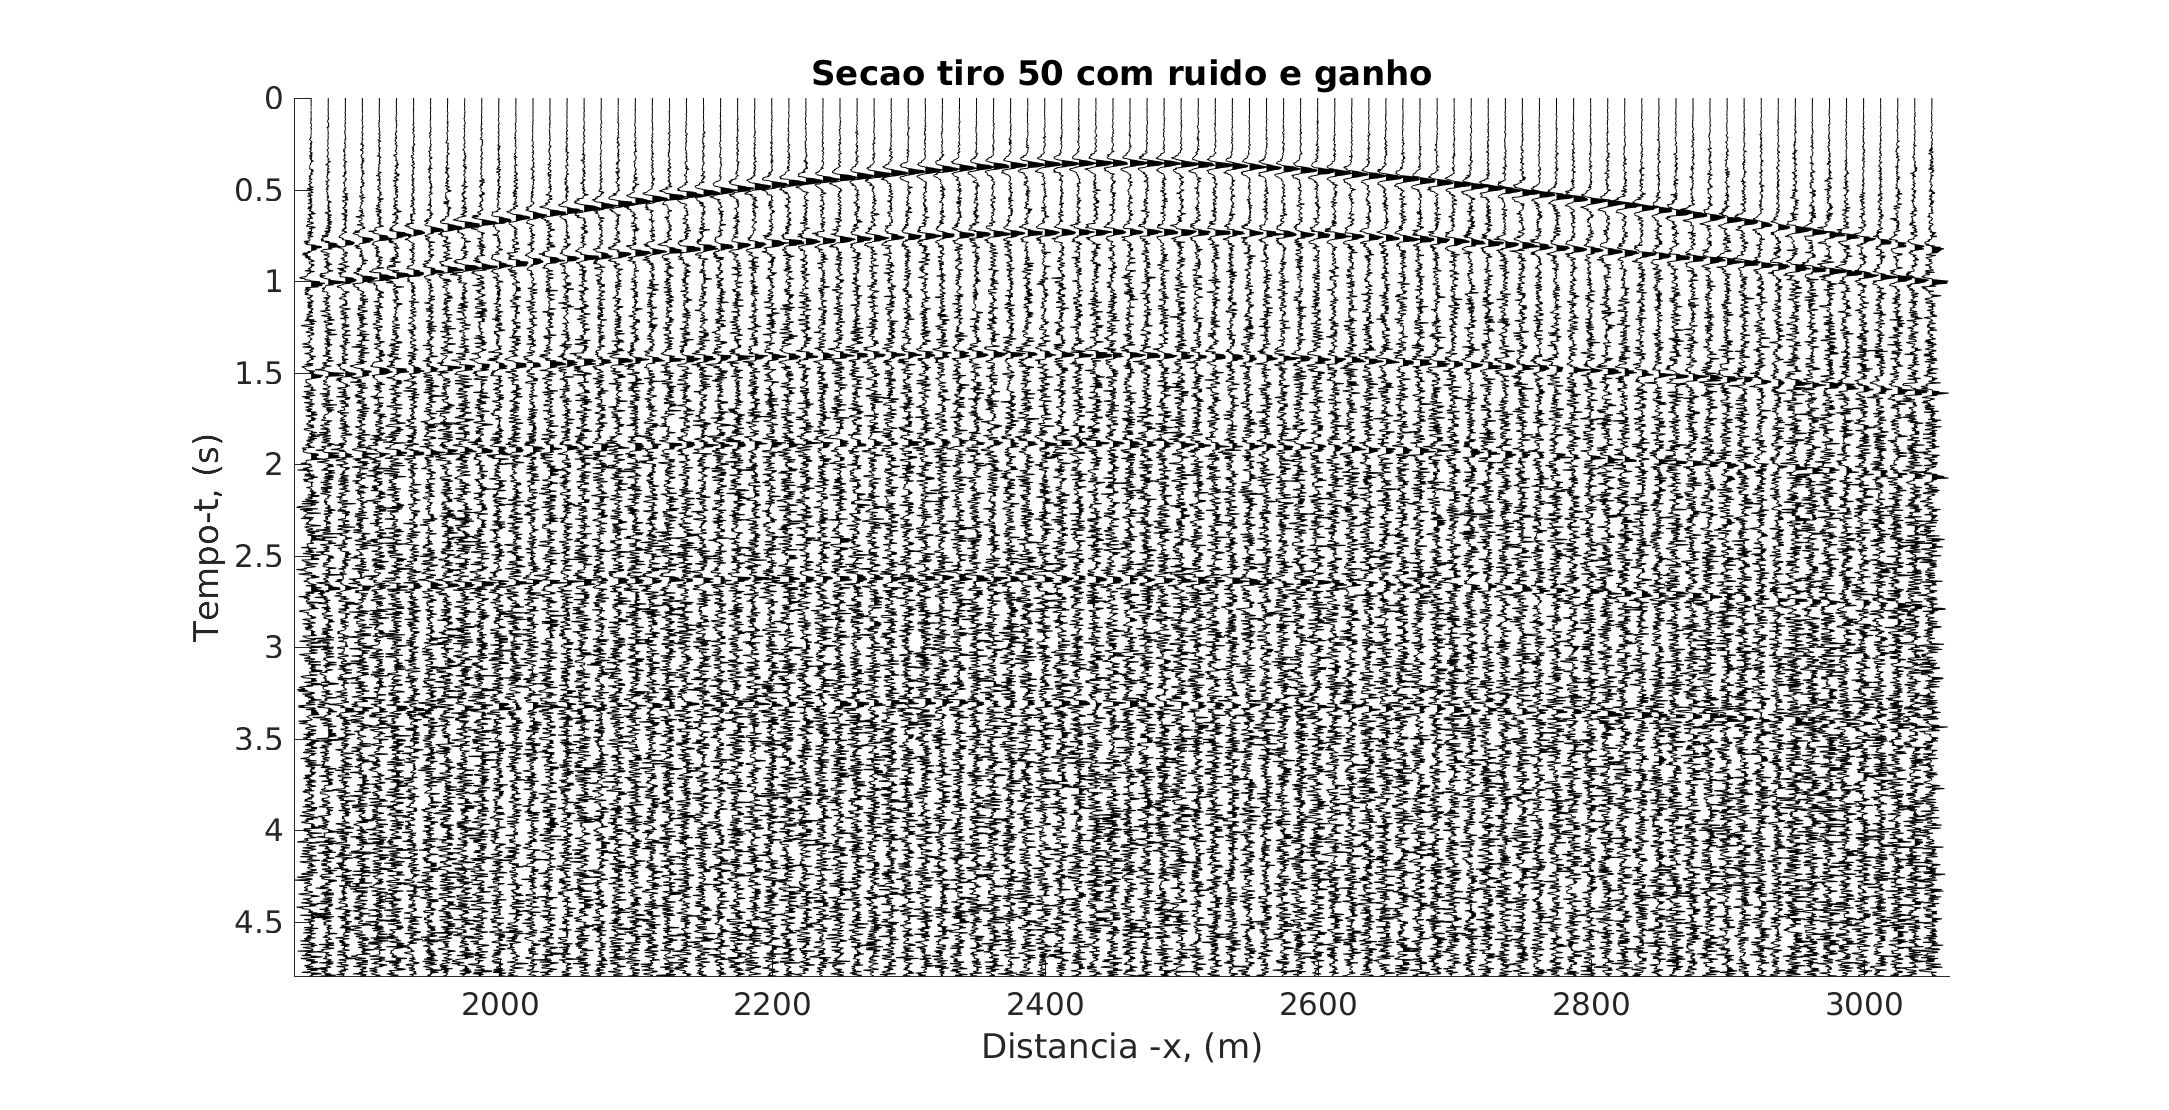
\includegraphics[totalheight=14cm]{figuras/cap3/secao_tiro50_ruido_gain.eps}
\caption{Seção tiro 50 com ruido e ganho, a informação e o ruído foram amplificados, os eventos de maior tempo foram ``mascarados'' com a amplificação da função ganho.}
\label{fig:tiro_50ruido_gain}
\end{figure}
\end{landscape}

\begin{landscape}
\begin{figure}[H]
\centering
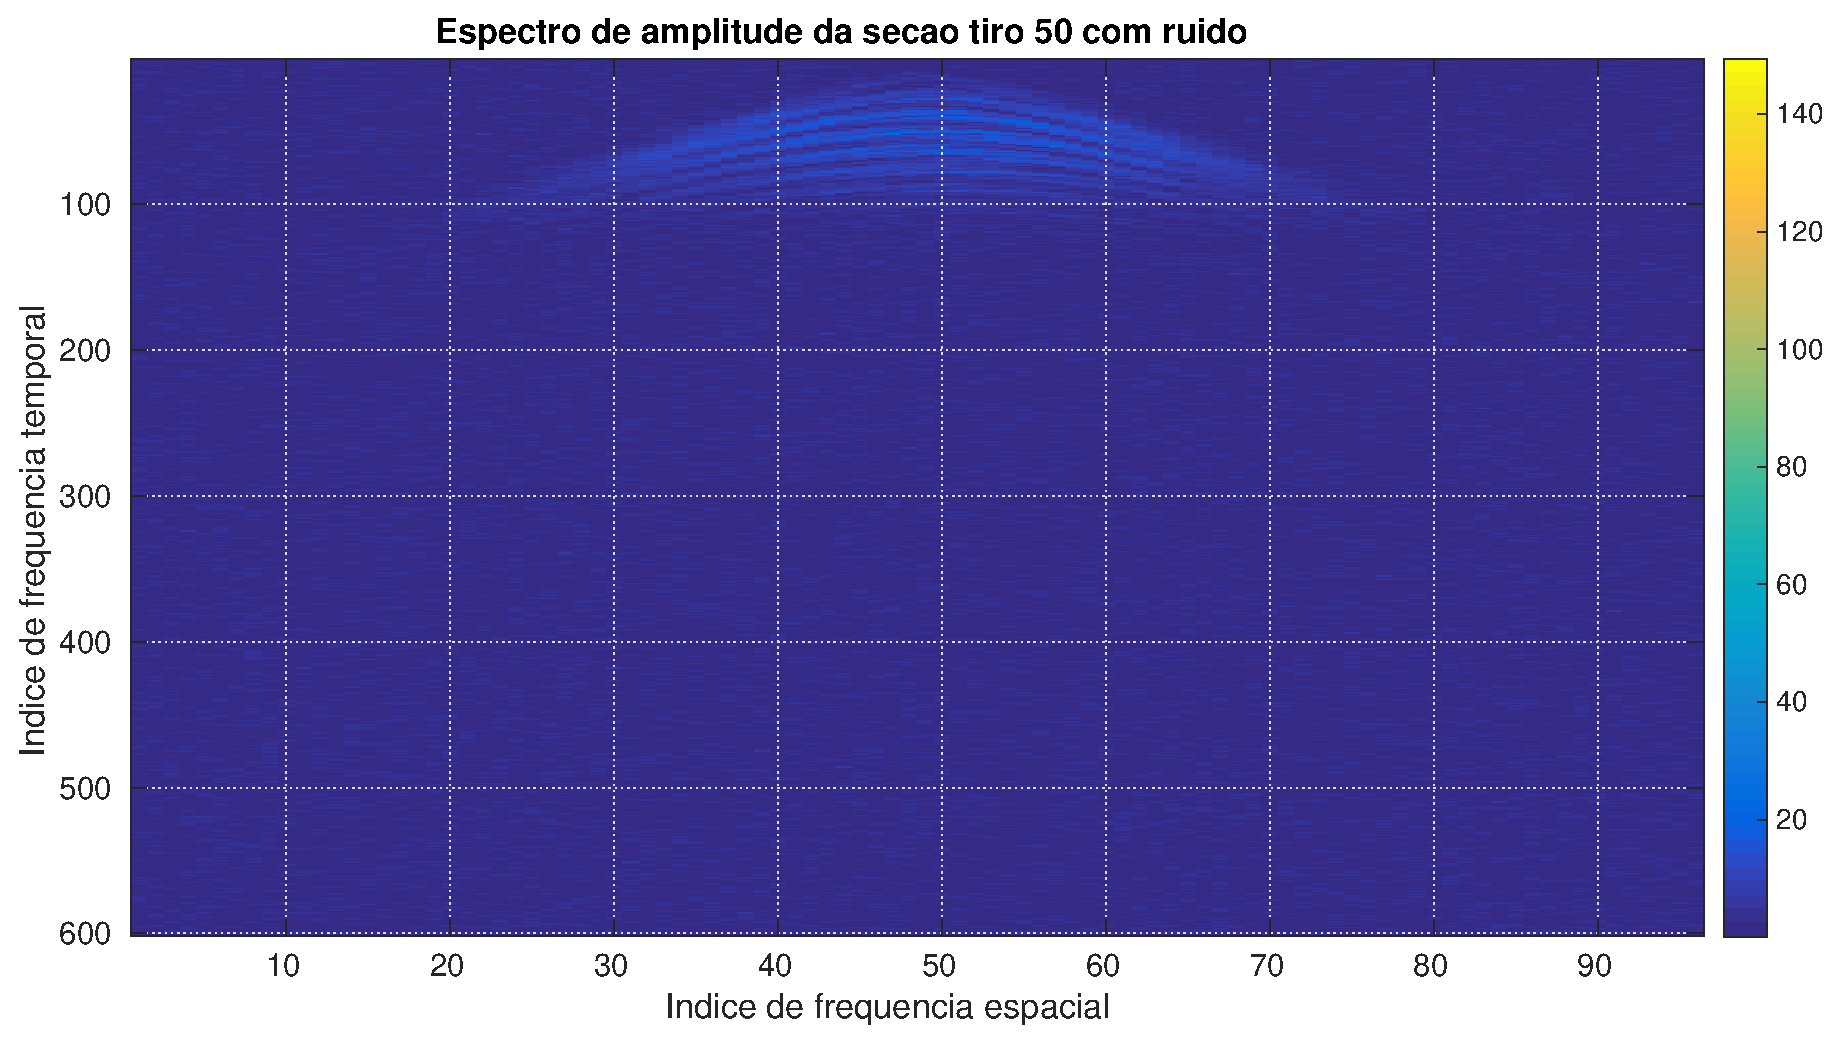
\includegraphics[totalheight=14cm]{figuras/cap3/espc_tiro50.eps}
\caption{Espectro da seção tiro 50 com ruído, este espectro não apresenta falseamento de informação tanto em $f_t$ (frequência temporal) quanto em $f_k$ (frequência espacial).}
\label{fig:espc_tiro50}
\end{figure}
\end{landscape}

\begin{landscape}
\begin{figure}[H]
\centering
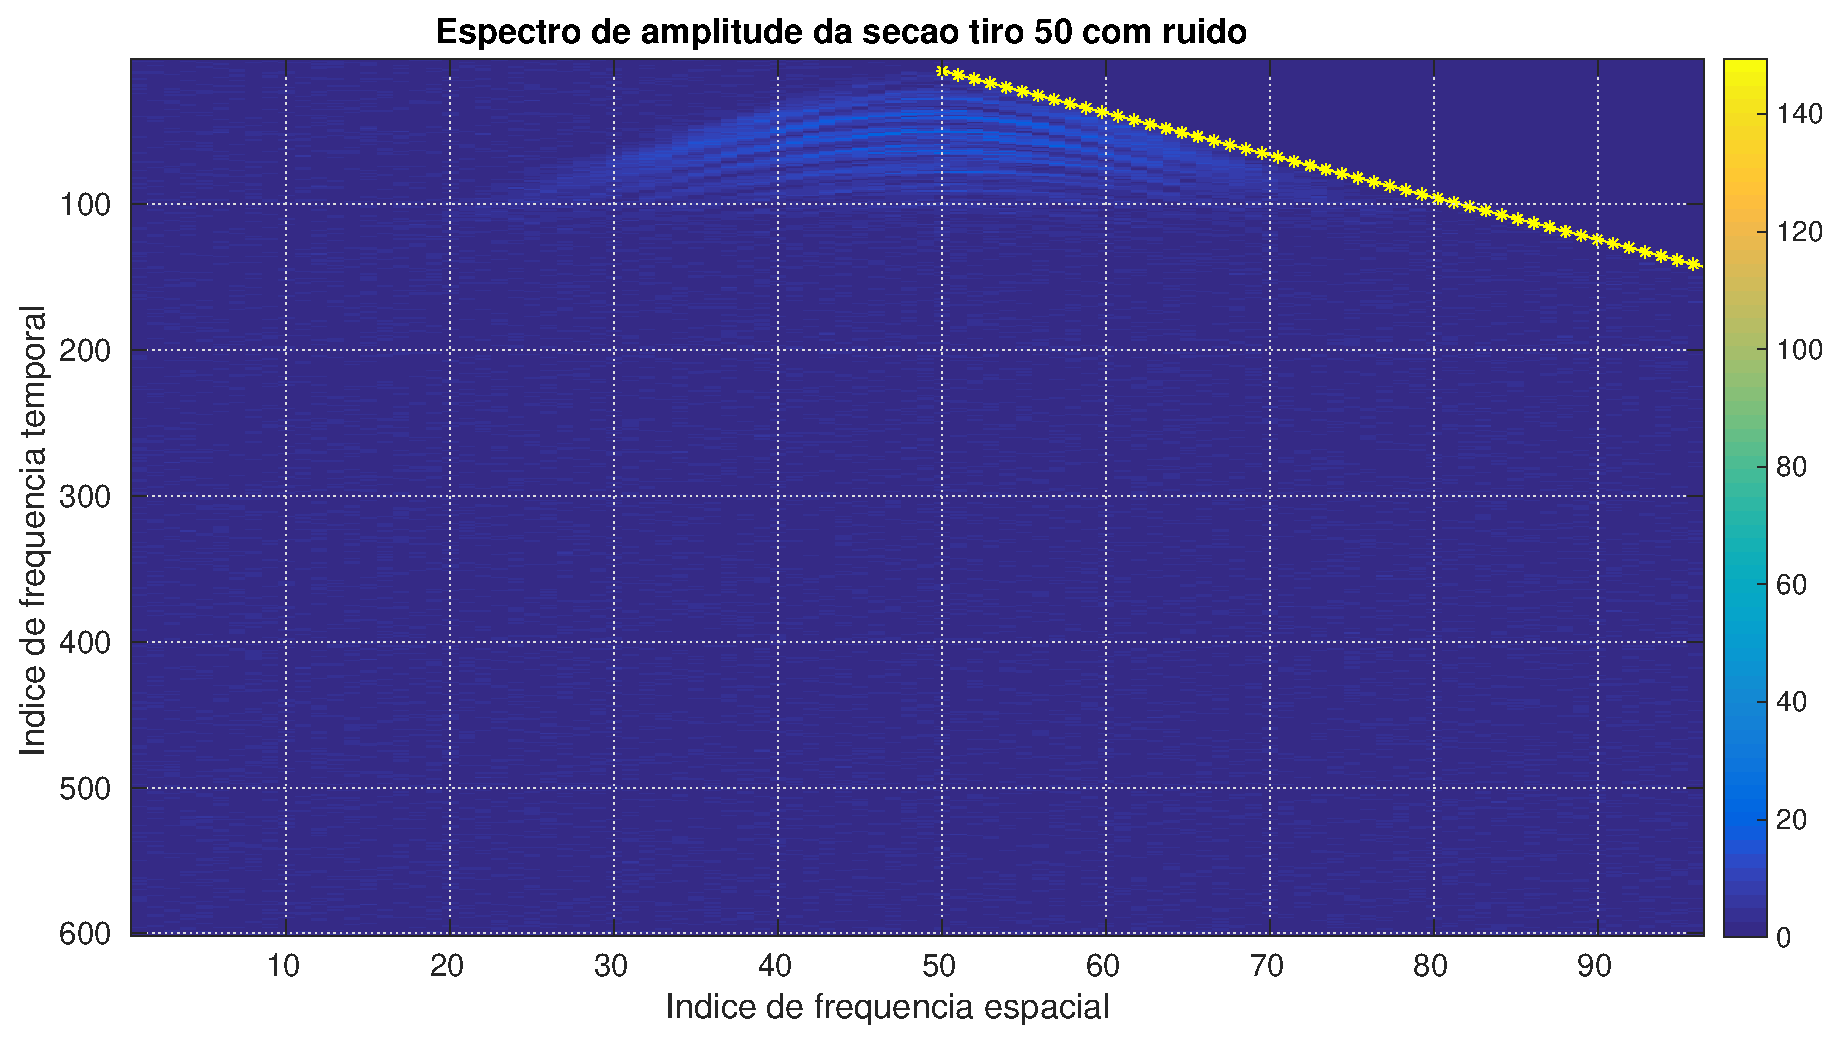
\includegraphics[totalheight=14cm]{figuras/cap3/espc_tiro50_c1.eps}
\caption{Seção tiro 50 com ruído após o primeiro corte (linha amarela) no espectro de amplitude.}
\label{fig:espc_tiro50_c1}
\end{figure}
\end{landscape}

\begin{landscape}
\begin{figure}[H]
\centering
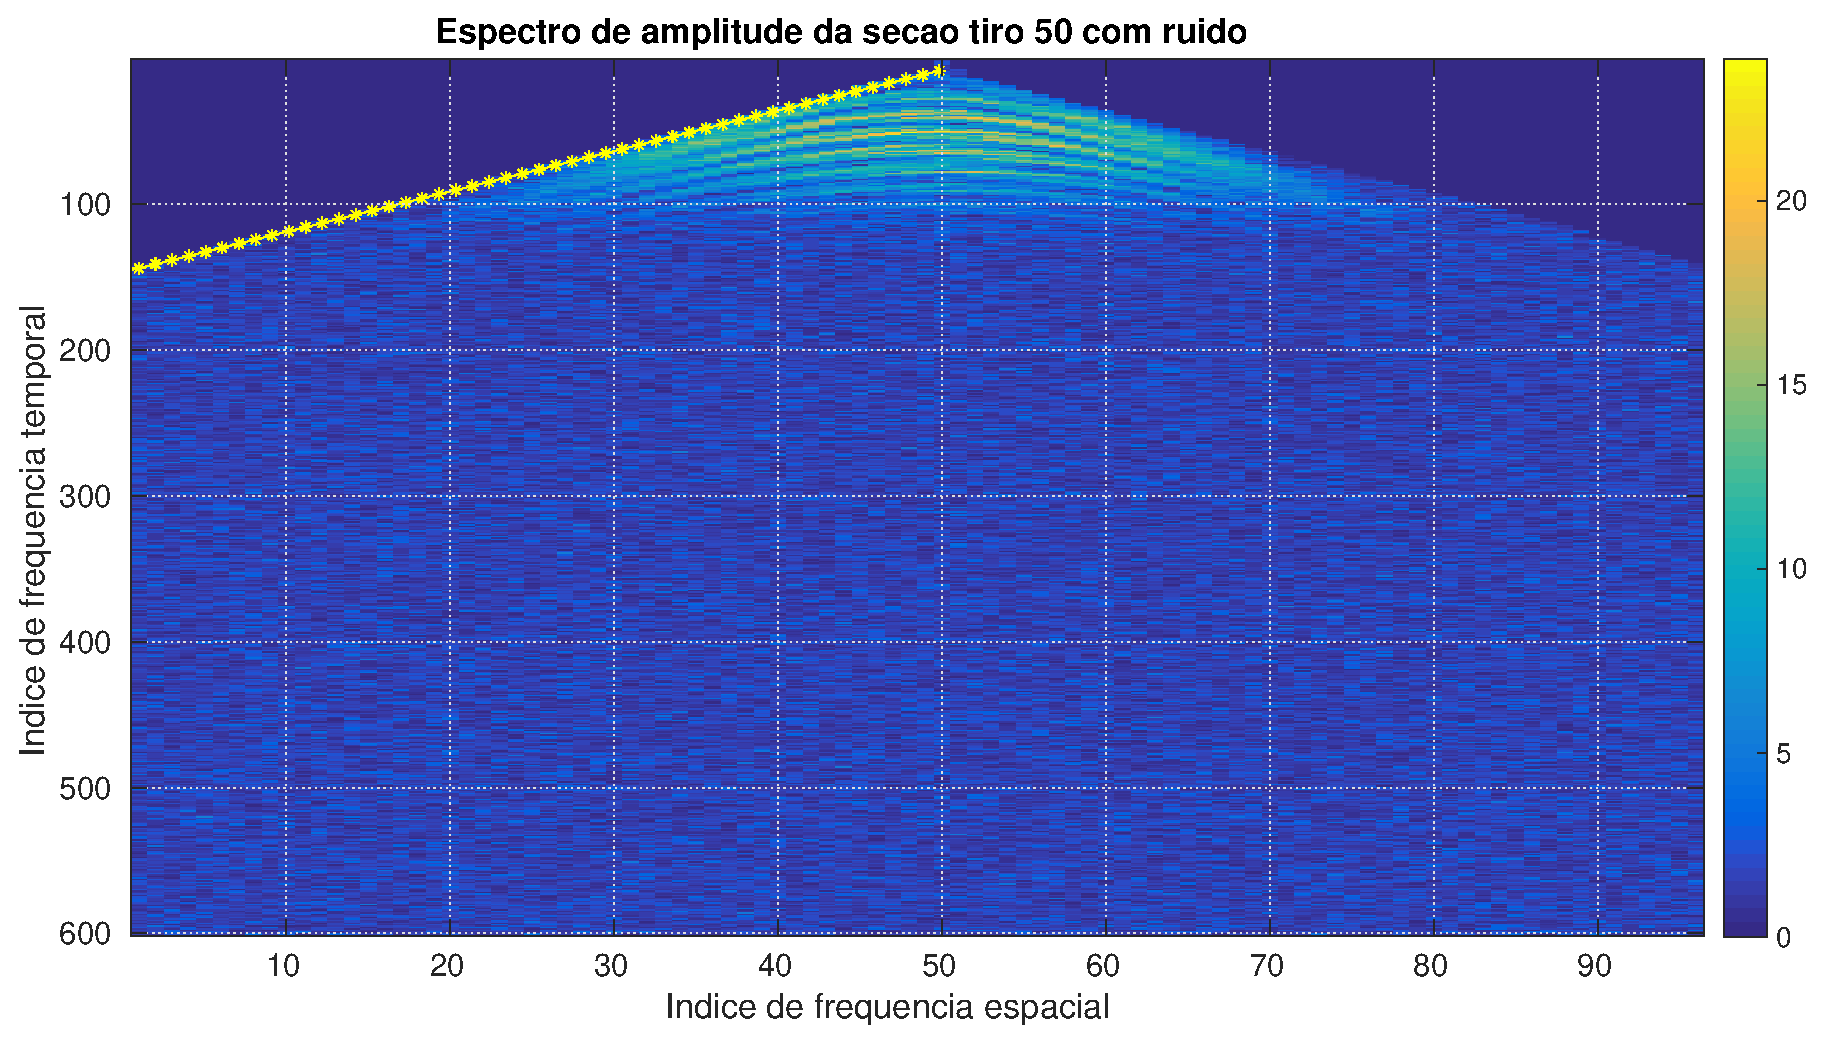
\includegraphics[totalheight=14cm]{figuras/cap3/espc_tiro50_c2.eps}
\caption{Seção tiro 50 com ruído após o segundo corte (linha amarela) no espectro de amplitude.}
\label{fig:espc_tiro50_c2}
\end{figure}
\end{landscape}

\begin{landscape}
\begin{figure}[H]
\centering
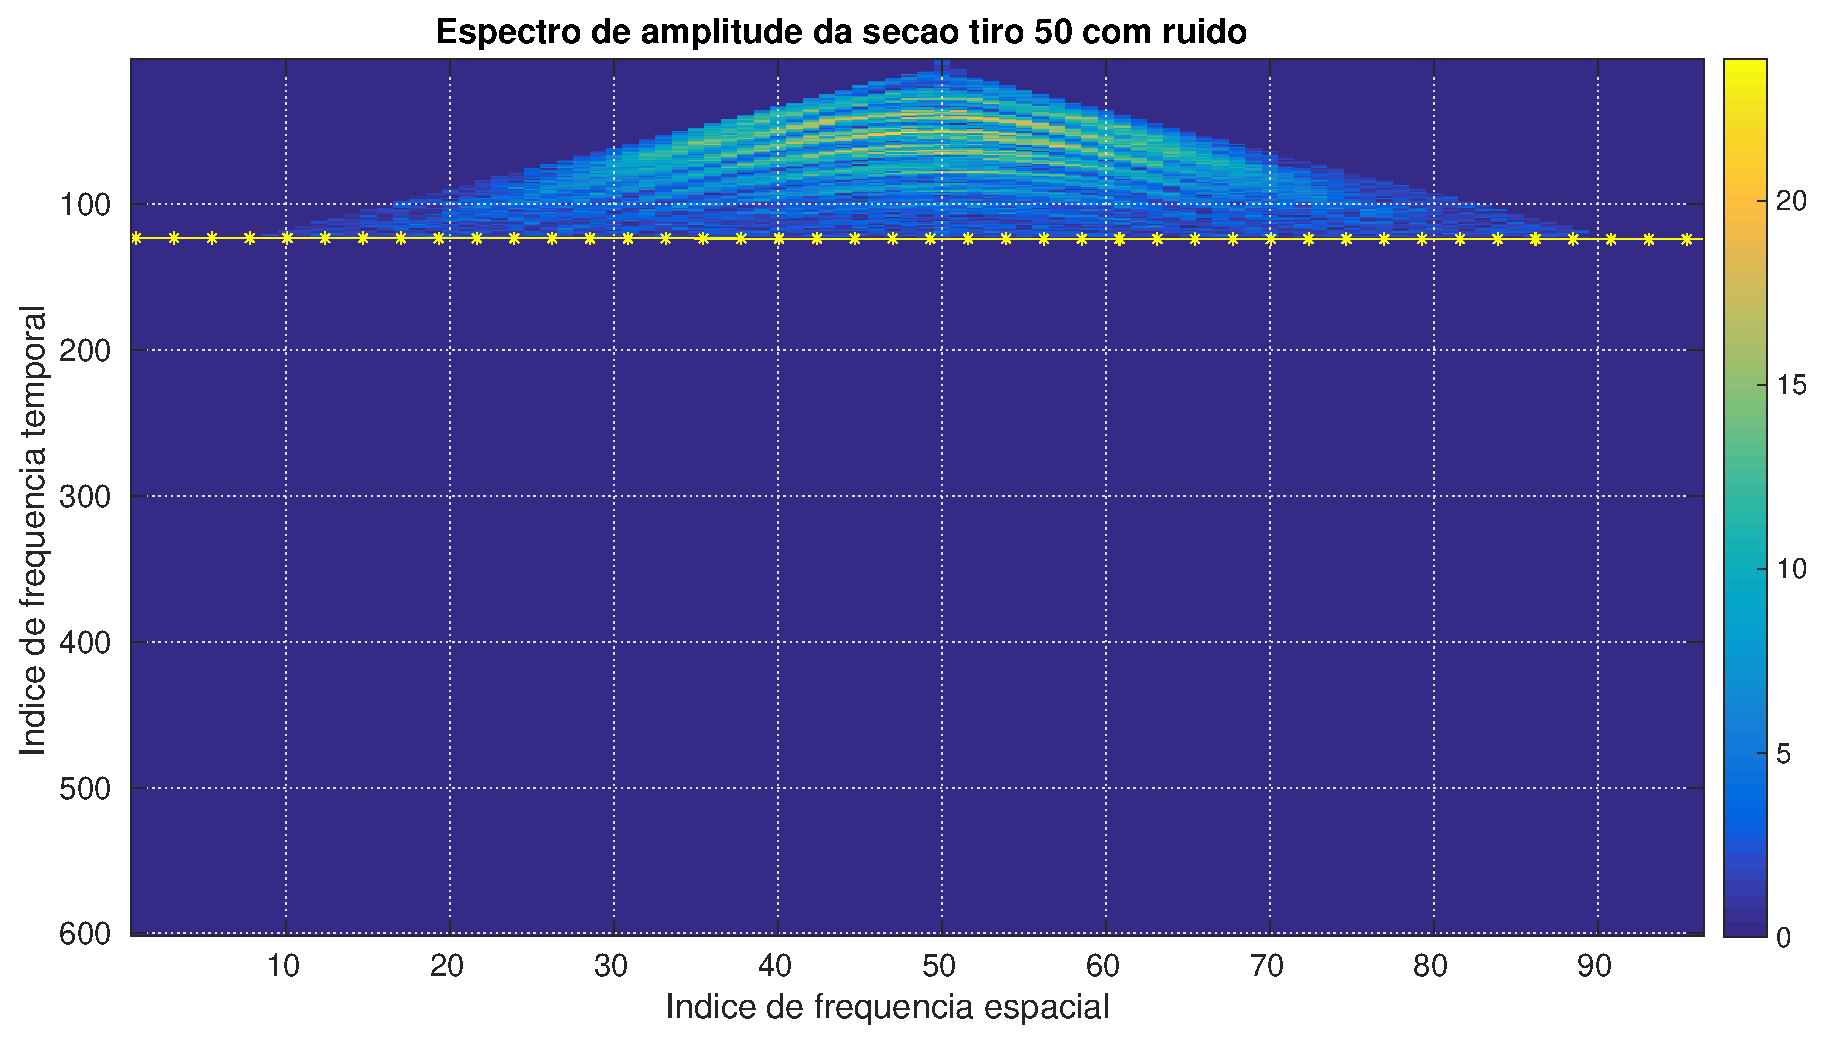
\includegraphics[totalheight=14cm]{figuras/cap3/espc_tiro50_c3.eps}
\caption{Seção tiro 50 com ruído após o terceiro corte (linha amarela) no espectro de amplitude.}
\label{fig:espc_tiro50_c3}
\end{figure}
\end{landscape}

\begin{landscape}
\begin{figure}[H]
\centering
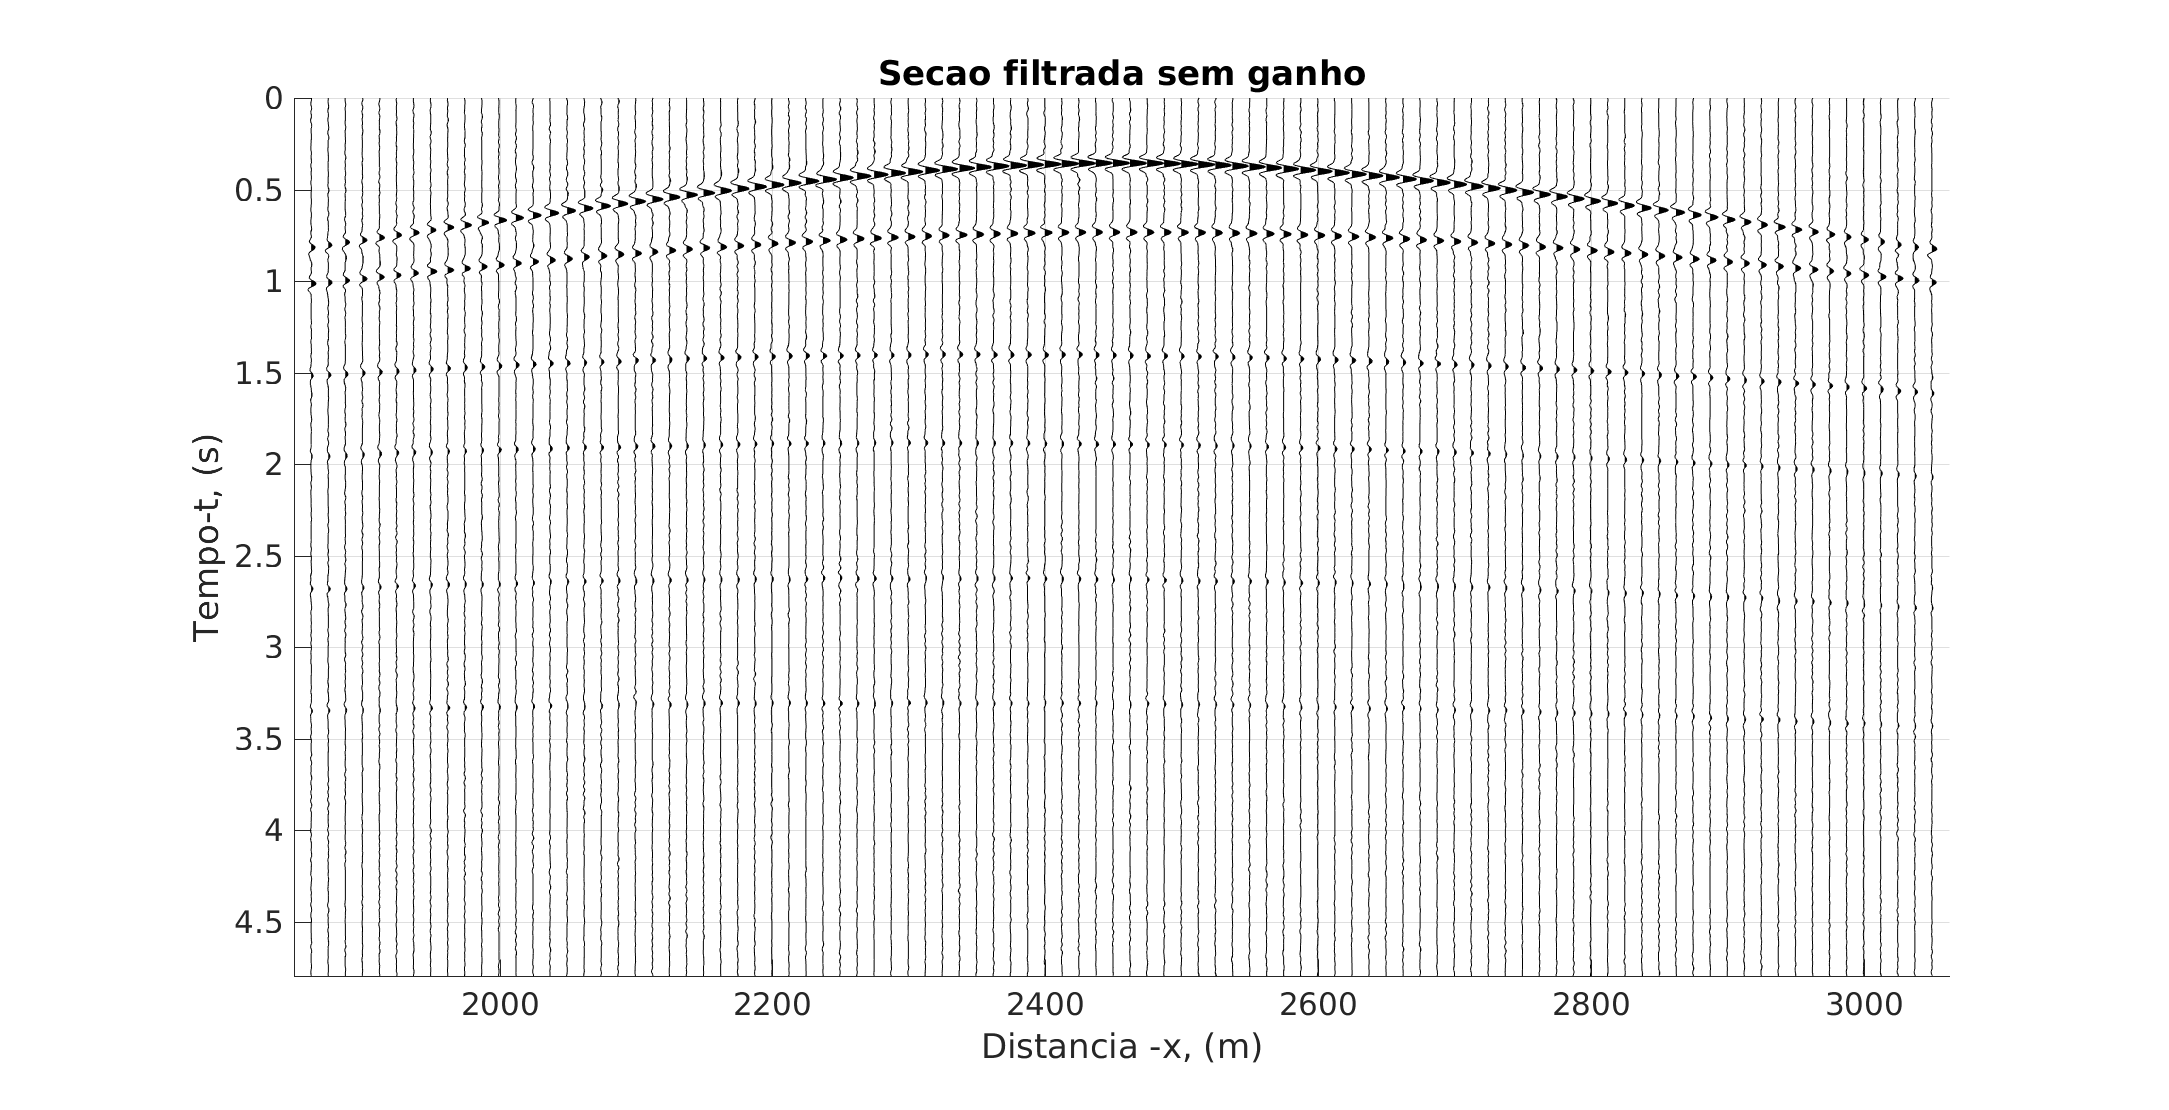
\includegraphics[totalheight=14cm]{figuras/cap3/secao_filtrada.eps}
\caption{Seção tiro 50 filtrada do ruído sem ganho, comparando a figura (\ref{fig:tiro_50ruido}) nota-se que a componente do ruído foi em grande parte removida após a filtragem F-K.}
\label{fig:secao_filtrada}
\end{figure}
\end{landscape}

\begin{landscape}
\begin{figure}[H]
\centering
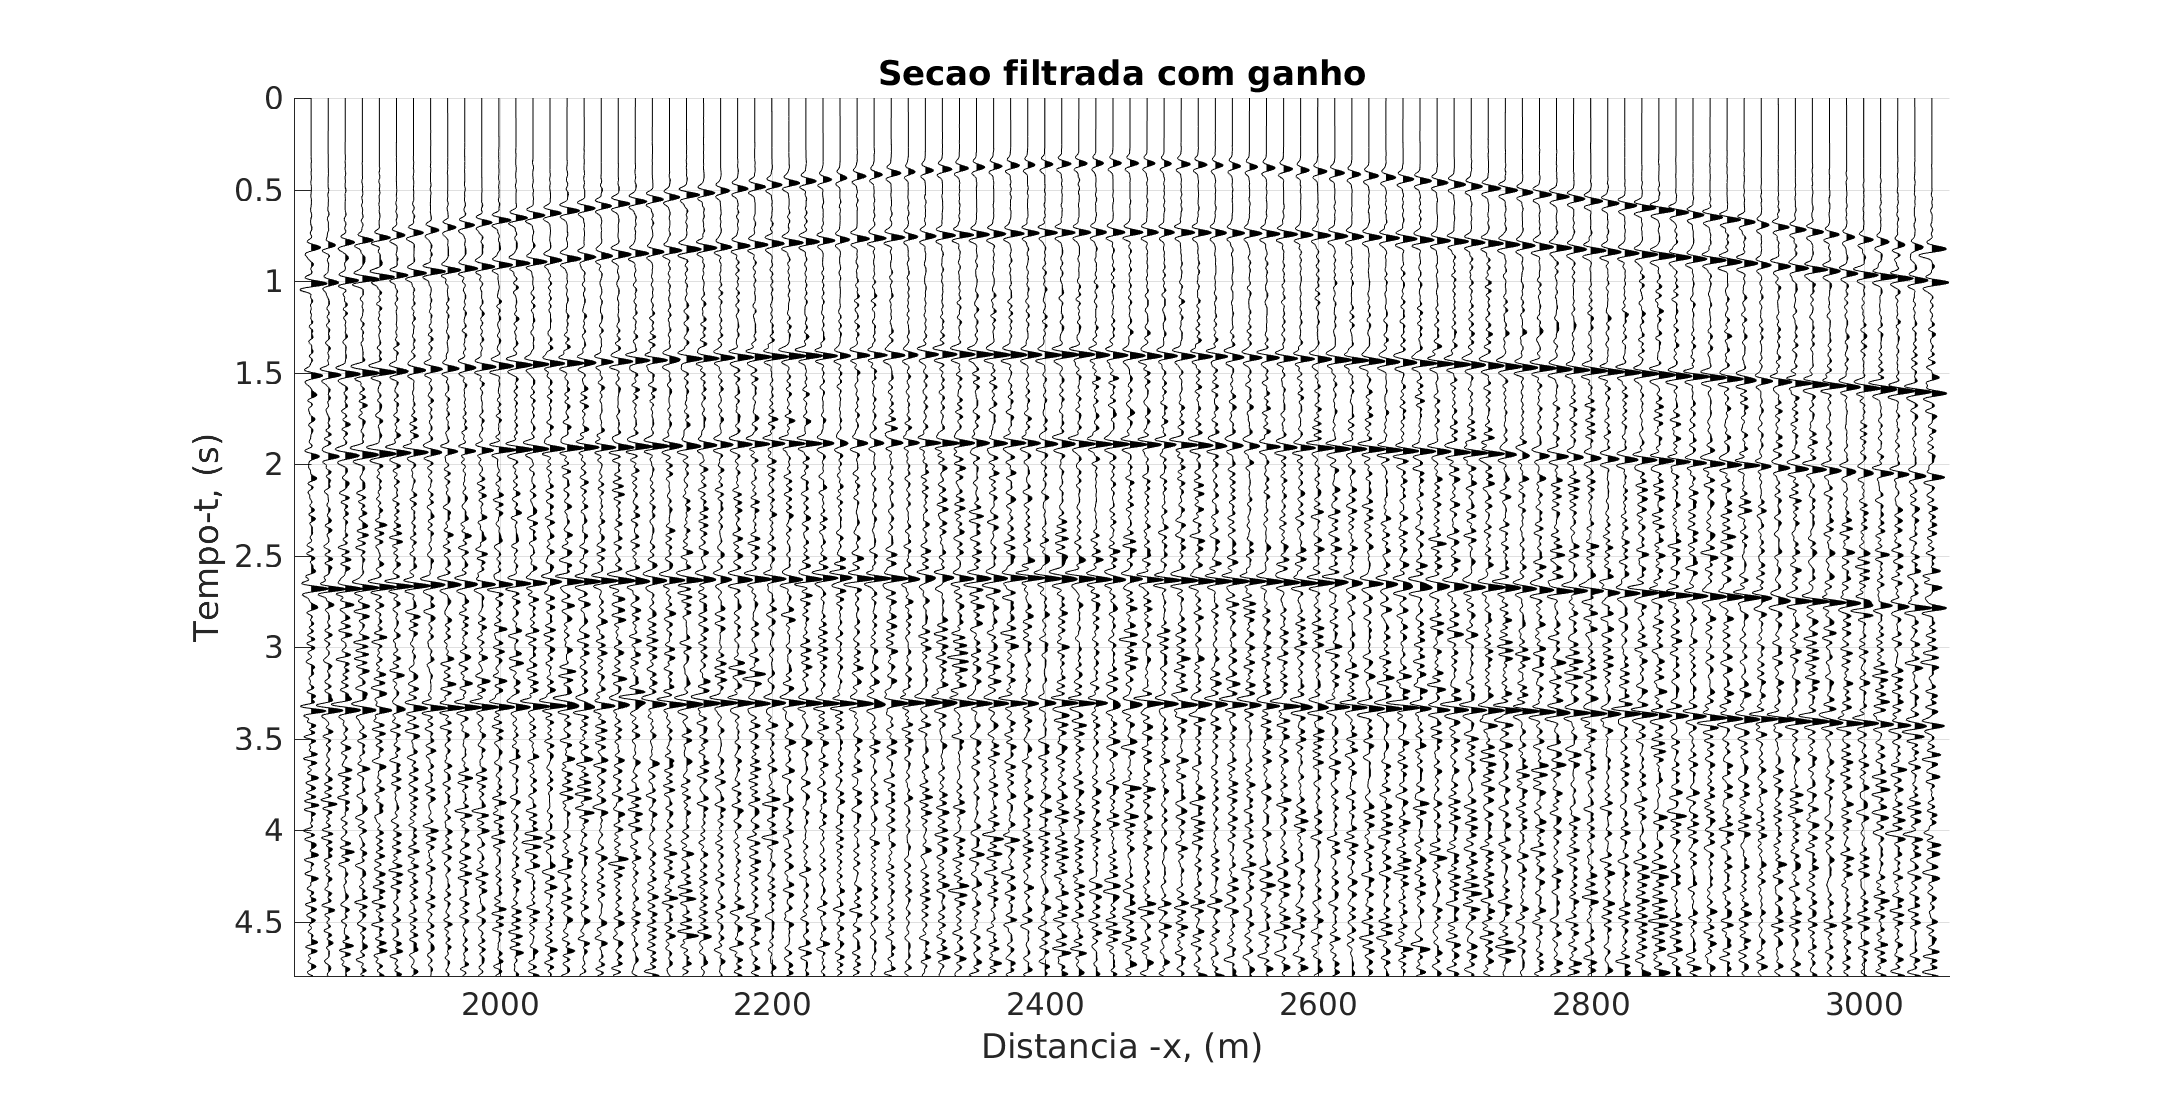
\includegraphics[totalheight=14cm]{figuras/cap3/secao_filtrada_gain.eps}
\caption{Seção tiro 50 filtrada do ruído com ganho, comparando a figura (\ref{fig:tiro_50ruido_gain}) nota-se que os eventos com maior tempo foram recuperados. O ganho amplificou tanto a informação de interesse (eventos) quanto o ruído.}
\label{fig:secao_filtrada_gain}
\end{figure}
\end{landscape}
\chapter{Experimentos numéricos}
\label{cap4}

\section{Modelo utilizado e aquisição}

 Os testes foram feitos utilizando um modelo com 9000 $m$ de comprimento e 3000 $m$ de profundidade. Quanto ao modelo de velocidade, foi utilizado o \textit{Marmousi} suavizado (Fig. \ref{fig:marmousi}). O modelo usado na Figura \ref{fig:modelortm} serviu para utilizar como entrada para o RTM. Foram utilizados 240 tiros nesse processo. O modelo utilizado para fazer a modelagem e o imageamento foi \textit{Intel(R) Core(TM) i5-7200U CPU 2.50GHz}, cujo possui 4 threads físicos.
 
 \begin{figure}[ht!]
	\centering
	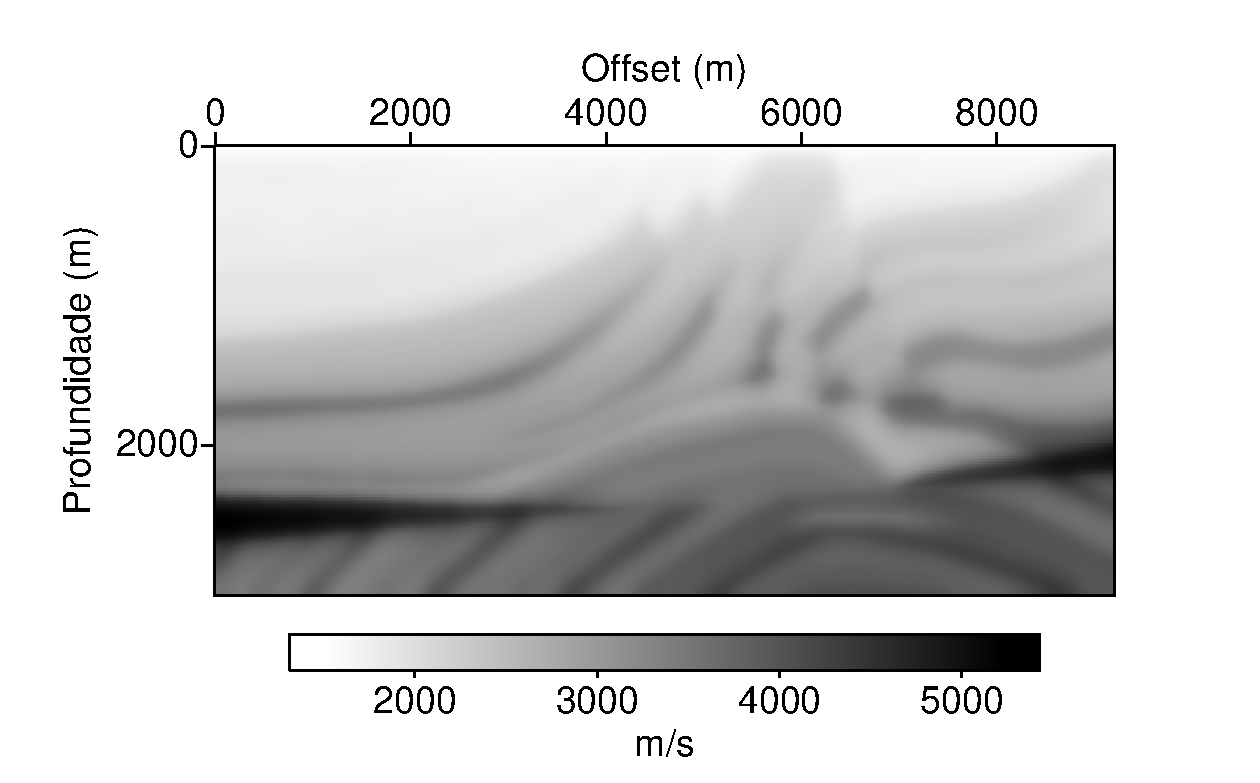
\includegraphics[width=15cm]{marmousi}
	\caption{Modelo de velocidade utilizado para a modelagem direta: modelo de Marmousi suavizado.} \label{fig:marmousi}
\end{figure} 
\begin{figure}[ht!]
	\centering
	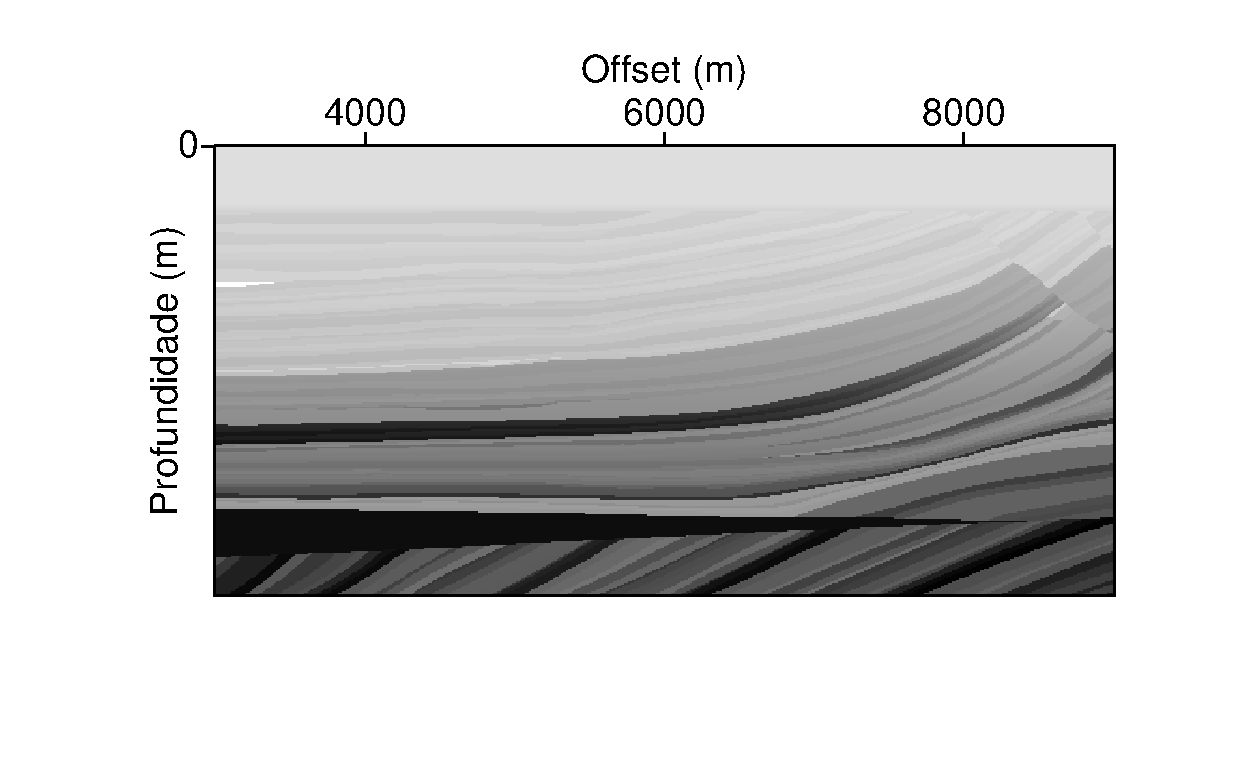
\includegraphics[width=15cm]{modelortm}
	\caption{Modelo utilizado para fazer a migração.} \label{fig:modelortm}
\end{figure} 
 \section{Resultados e discussões}
 
 Após feito o processo de modelagem e aplicado o RTM, foi gerada a Figura \ref{fig:rtm}. 
 \begin{figure}[ht!]
 	\centering
 	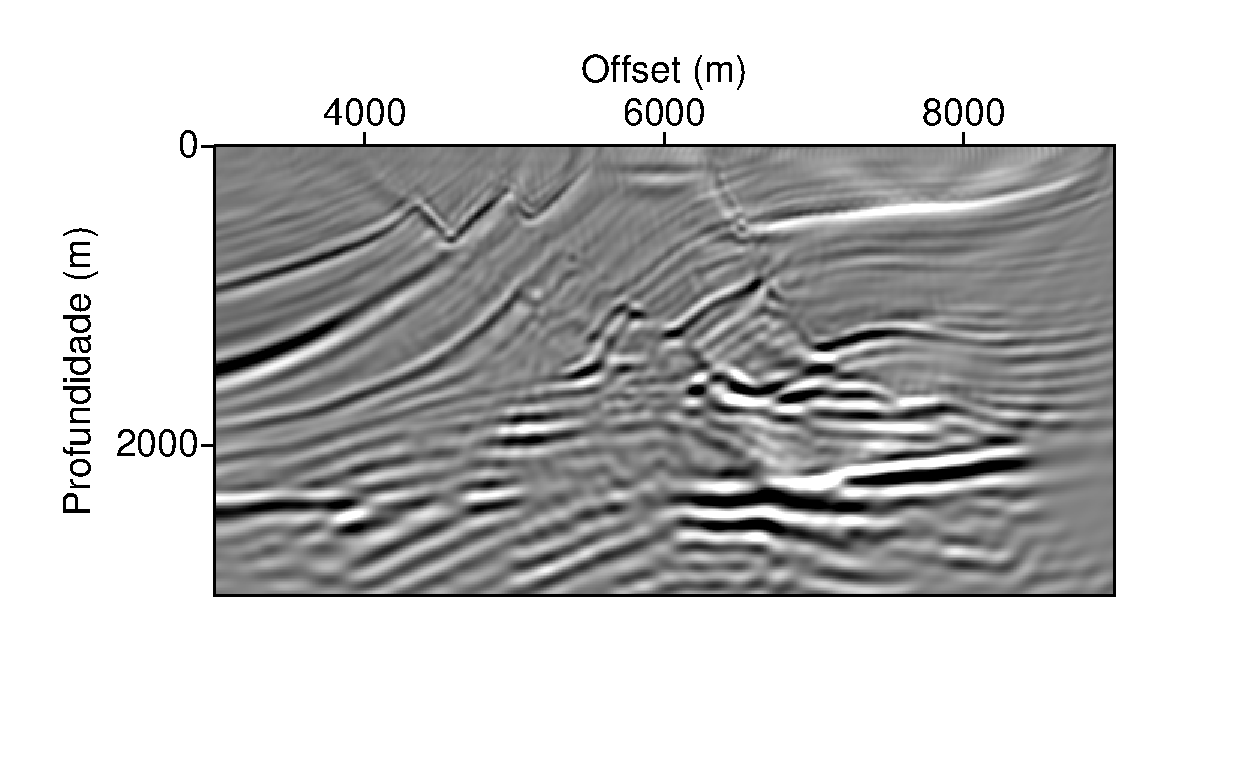
\includegraphics[width=15cm]{rtmfinal}
 	\caption{Imagem migrada do modelo de Marmousi filtrada.} \label{fig:rtm}
 \end{figure} 
 Na Figura \ref{fig:rtm}, nota-se que os eventos estão bem destacados, sem a presença de reflexões. Portanto, é possível analisar que esta técnica de imageamento teve bom funcionamento.
 
  Quanto ao custo computacional do RTM, foram necessárias aproximadamente 80 horas para gerar a Figura \ref{fig:rtm}. Caso não houvesse sido utilizada a paralelização, a tendencia era de maior custo computacional.









\chapter{MIGRAÇÃO POR DIFRAÇÃO}
\label{cap5}

% \chapter{DISCUSSÕES E CONCLUSÕES}
\label{cap6}


%%%%%%%%%% - BIBLIOGRAFIA - %%%%%%%%%%%%%%%%%%%%
\bibliography{biblio}
\bibliographystyle{cpgf_seg} 


%%%%%%%%%% - APENDICES E ANEXOS - %%%%%%%%%%%%%%%%%%%%
\apendices 
\appendix
% \addcontentsline{doc}{chapter}{Ap\^endices}
\label{apendice}

\chapter{ Auto convoluções e espectro de amplitude.}
\label{apendice_A}

Este código de matlab foi escrito para fazer todo o trabalho para o curso de "Processamento de Sinais Digitais.



\lstinputlisting[language=bash,breaklines=true]{codes/projeto.m}


%\anexos
%\include{Cap_4_apendice}


\end{document}
